%%%%%%%%%%%%%%%%%%%%%%%%%%%%%%%%%
%% usmthesis.cls 2016/12/08 version V1.7.
%%
%% IMPORTANT MESSAGE (Dec 2016)
%% Due to the recent numerous changes requested by IPS, USM to different
%% candidates -- often conflicting even within the same week -- without much
%% consistency nor in black in white, I have found it increasingly difficult
%% to maintain a coherent version. I have therefore decided to provide some
%% options that seem to be favored by IPS on different occasions; but will no
%% longer update the template until an updated formatting guidelines with clear
%% instructions and concrete samples is published.
%%
%% THERE WILL BE NO FURTHER UPDATES UNTIL IPS-USM PUBLISHES AN OFFICIAL
%% UPDATED FORMATTING GUIDELINES WITH CONCRETE, CLEAR INSTRUCTIONS.
%%
%% Individual requests for help to modify this version for your needs will be
%% handled on a case by case basis, depending on my mood, perhaps for a fee.
%% Requests for help to modify past versions will NOT be entertained.
%% Please read http://tex.my/how-to-ask-for-latex-related-help-effectively/.
%%
%% (Yes I'm that tired and frustrated. I know everyone just want to graduate,
%% but I am by now genuinely put off by the tone of some requests with rude
%% attitudes, unclear descriptions, flip-flopping conditions, etc for something
%% that was originally for my own use.)
%%
%% Usmthesis _was_ fun; but it has ceased to be so for me.
%%
%% Submit a git pull request on https://github.com/liantze/usmthesis
%% if you wish to contribute your changes. No timeframe is set for approvals.
%% I cannot check through any edited usmthesis.cls of any version without
%% CVS.
%%
%% Oh and if you'd like to adapt this template (the .cls and/or the .tex) for
%% your institution, that's perfectly fine, but at least keep the license
%% (LPPL 1.3) and the original author (me) won't you? It's just normal decency.
%% THANK you. :-)
%%%%%%%%%%%%%%%%%%%%%%%%%%%%%%%%%

%% If you prefer -- and have been allowed -- to use
%% Arial, then
%% \documentclass[arial]{usmthesis}
%% It's not really Arial, it's a Helvetica look-alike,
%% but if you're not a designer nor a typographer, you
%% probably can't tell the difference (I can't either)
%%
%% OTHER IMPORTANT OPTIONS:
%% singespacetitle - Make title on cover and title
%%                   page single-spaced.
%%
%% chapnumwords — Make chapter titles be `Chapter One'
%% tocchapnumwords — Make the ToC use `Chaper One' too
%%   (Engineering IPS seems to like the above two settings)
%%
%% tocpage   These options will add a ``Page'' label at the
%% lotpage   top of the Table of Contents, List of Tables,
%% lofpage   List of Figures and List of Plates respectively.
%% loppage   I don't know lah, one moment IPS says must add at
%%           the top of all these lists; one month later say
%%           only the ToC, a few months later say don't add at all.
%%           Find, mix-and-match yourself based on the instrustions you got.
%%
%% tocCAPSfront - Sometimes IPS wants the ``Table of Contents'', ``List of
%%                Figures'', ``Abstract'' etc to be all-caps in the ToC;
%%                sometimes they don't. Use this option to make them ALL CAPS.
%%
%% tocCAPSref - Similar to the above but for the ``References''.
%% tocCAPSapp - Similar to the above but for the ``Appendices''.
\documentclass[
singlespacetitle, % Make title on cover page singlespaced
% chapnumwords,tocchapnumwords,  %% ``Chapter One'' I think Engineering like this
tocpage,  % Put ``Page'' at top of ToC. Add lotpage, lofpage if
          % ``Page'' is also needed for LoT and LoF.
% tocCAPSfront, % Make ``List of Tables'' etc in ToC CAPS
% tocCAPSref, % Make ``References'' in ToC CAPS
% tocCAPSapp, % Make ``Appendices'' in ToC CAPS
]{usmthesis}

%%%%%%%%%%%%%%%%%%%%%%%%%%%%%%%%%%%%%%%%%%%%%%%%%%%%%%%
% This is usmthesis.tex, 6 Dec 2016. READ THE COMMENTS.
% Some formattings are easiest changed by uncommenting
% some lines in this .tex file or by changing certain
% options.
%
% Created by Lim Lian Tze (Ph.D.)
% liantze@gmail.com
% http://liantze.penguinattack.org.
%%%%%%%%%%%%%%%%%%%%%%%%%%%%%%%%%%%%%%%%%%%%%%%%%%%%%%%
% \documentclass[article]{memoir}
% \feetbelowfloat

\usepackage{pdfpages}
\usepackage{afterpage}

% Set font size to 13pt
\usepackage{scrextend}
\changefontsizes{13pt}

%% Example of loading other packages that you may require.
%% I'm loading the marvosym package so that I can produce a
%% smiley face with the command \Smiley.
\usepackage{marvosym}

%% Also, the enumitem package is great for customising
%% list environments.
\usepackage{enumitem}
\usepackage{tabu}
\usepackage{booktabs}
\usepackage{calligra}
\usepackage{multirow}
\usepackage{multicol}
\usepackage{bm}
\usepackage{bibentry}



%% Listings is a nice package for typesetting code
%% listings. Other possible packages include fancyvrb,
%% minted, etc.
\usepackage{listings}
\lstset{basicstyle=\ttfamily,breaklines=true}

%% For those who need to produce algorithms and pseudocode.
%% There are a number of different packages available, but
%% unfortunately they tend not to work well together!
%% I'm using algorithmicx, specifically algpseucode, here.
\usepackage{algpseudocode}
\usepackage{algorithm}
\usepackage{indentfirst}

%% Enter particulars about your thesis HERE
% Your Name
\author{HUỲNH LÂM HẢI ĐĂNG - 19125003\\
	HỒ THỊ NGỌC PHƯỢNG - 19125014}

% English title of your thesis
\title{ENHANCING VIDEO SUMMARIZATION WITH CONTEXT AWARENESS}
% Malay title of your thesis
\titlems{Penulisan Tesis dengan LaTeX}
% Year submitted
\submityear{2023}
% Month submitted
\submitmonth{July}
%% Choose only 1 degree type! :-)
\degreetype{BACHELOR OF SCIENCE IN COMPUTER SCIENCE}
% \degreetype{Master of Science}
\lecturer{ASSOC.PROF. TRẦN MINH TRIẾT - PROF.~LÊ~TRUNG~NGHĨA}

%%%%%%%%%%%%%%%%%%%%%%%%%%%%%%%%%%%%%%%%%%%%%%%%%%%%%%%
% You can comment out the following line if you don't have a
% "List of Own Publications". And make it all caps yourself
% if it needs to be all caps in the ToC.
%%%%%%%%%%%%%%%%%%%%%%%%%%%%%%%%%%%%%%%%%%%%%%%%%%%%%%%
\newcites{own}{List of Publications}

\usepackage[plainpages=false,bookmarksnumbered,
bookmarksdepth=section,breaklinks=true]{hyperref}
%%%%%%%%%%%%%%%%%%%%%%%%%%%%%%%%%%%%%%%%%%%%%%%%%%%%%%%
% Options for generating hyperlinks when using pdfLaTeX
%%%%%%%%%%%%%%%%%%%%%%%%%%%%%%%%%%%%%%%%%%%%%%%%%%%%%%%

\hypersetup{
    colorlinks,
    citecolor=black,
    filecolor=black,
    linkcolor=black,
    urlcolor=black
}

\ifpdf
  \makeatletter
  \hypersetup{hypertexnames=false,%
    pdfauthor={\@author},pdftitle={\@title}}
  \makeatother
\fi

\usepackage{ragged2e}
\usepackage{tikz}
\usepackage{multido}
\usetikzlibrary{calc}
\usepackage{longtable}
\usepackage{makecell}
% \usepackage{biblatex}
\begin{document}

%%%%%%%%%%%%%%%%%%%%%%%%%%%%%%%%%%%%%%%%%%%%%%%%%%%%%%%
% Default bibliography style is apa (using
% \RequirePackage[natbibapa]{apacite} in the class file).
%
% If you prefer the number system though, use bibliography
% style "plainnat" for [1][2][3] or "alpha" for [Jon94] (the label
% will be auto-generated).
%%%%%%%%%%%%%%%%%%%%%%%%%%%%%%%%%%%%%%%%%%%%%%%%%%%%%%%
% \bibliographystyle{apacite}
% \bibliographystyleown{apacite}
% \bibliographystyle{plainnat}
% \bibliographystyleown{plainnat}
\bibliographystyle{unsrtnat}
\bibliographystyleown{unsrtnat}
\frontmatter

%%%%%%%%%%%%%%%%%%%%%%%%%%%%%%%%%%%%%%%%%%%%%%%%%%%%%%%
% Inserts the cover page (the hard cover with gold-lettering)
% and the title page
%%%%%%%%%%%%%%%%%%%%%%%%%%%%%%%%%%%%%%%%%%%%%%%%%%%%%%%
\makecover


%%%%%%%%%%%%%%%%%%%%%%%%%%%%%%%%%%%%%%%%%%%%%%%%%%%%%%%
% MAKE SURE YOU HAVE A acknowledgements.tex FILE
%%%%%%%%%%%%%%%%%%%%%%%%%%%%%%%%%%%%%%%%%%%%%%%%%%%%%%%
\chapter*{COMMENT OF THESIS'S ADVISOR}
\begin{tikzpicture}[remember picture, overlay]
  \draw[line width = 1pt] ($(current page.north west) + (1.2in,-1in)$) rectangle ($(current page.south east) + (-0.7in,1in)$);
\end{tikzpicture}
\multido{}{20}{\noindent\makebox[\linewidth]{\dotfill}\endgraf}
\chapter*{COMMENTS OF THESIS'S REVIEWER}
\begin{tikzpicture}[remember picture, overlay]
  \draw[line width = 1pt] ($(current page.north west) + (1.2in,-1in)$) rectangle ($(current page.south east) + (-0.7in,1in)$);
\end{tikzpicture}
\multido{}{20}{\noindent\makebox[\linewidth]{\dotfill}\endgraf}

\chapter{Acknowledgement}

% First of all, we would like to express our sincere gratitude and appreciation to our thesis advisor Assoc. Prof. Trần Minh Triết for the continuous support of our study and research. With his patience, conscientious guidance, enthusiast support, we have acquired valuable knowledge in the fields of Machine Learning, Deep Learning, Computer Vision. Our thesis could not completed without his friendly guidance and expert advice.

% We also would like to say thanks to Dr. Lê Trung Nghĩa for his extended discussions and valuable suggestions which have contributed greatly to the improvement of the thesis.

% Moreover, we are grateful to all of our lecturers in the Faculty in Information and Technology, University of Science, VNUHCM. They have built us a solid foundation in Computer Science, especially in Artificial Intelligence field, which makes it easier for us to acquire deeper knowledge to finish our thesis.

% Besides, we are really thankful for our generous colleagues at the SELAB, University of Science: Trương Thành Đạt, Bùi Ngọc Minh, Đỗ Trọng Lễ, Lương Quốc An, Trần Mai Khiêm who are always here to help us and give valuable comments whenever we need their support.   

% Last but not least, our deepest gratitude goes to all of our parents. It would not be possible to write this thesis without their immeasurable support, caring and encouragement throughout our education. 

\begin{flushright}
\begin{minipage}{8cm}
\centering
Authors

Huỳnh Lâm Hải Đăng \& Hồ Thị Ngọc Phượng
\end{minipage}
\end{flushright}
\chapter{Thesis Proposal}
\begin{longtable}{|l|c|}
\hline
\multicolumn{2}{|m{\linewidth}|}{\textbf{Thesis title}: ENHANCING VIDEO SUMMARIZATION WITH CONTEXT AWARENESS
}\\
\hline
\multicolumn{2}{|m{\linewidth}|}{\textbf{Advisors}: Assoc.Prof. Trần Minh Triết, Dr. Lê Trung Nghĩa} \\
\hline
\multicolumn{2}{|m{\linewidth}|}{\textbf{Duration}: January 1\textsuperscript{st}, 2023 to August 14\textsuperscript{th}, 2023}\\
\hline
\multicolumn{2}{|m{\linewidth}|}{\textbf{Students}: Huỳnh Lâm Hải Đăng (19125003) - Hồ Thị Ngọc Phượng (19125014)}\\
\hline
\multicolumn{2}{|m{\linewidth}|}{\textbf{Theme of Thesis}: theoretical research, proposed improvements.}\\
\hline
\multicolumn{2}{|m{\linewidth}|}{\textbf{Content}:\par
We aim to propose a novel approach for improving video summarization quality by integrating context awareness. We also aim to propose an evaluation metric that better suits the practical use of problem in real life.\par
The details include:
\begin{itemize}
  \item Literature Review and Proposal Writing \begin{itemize}
    \item Conduct a comprehensive literature review on video summarization, identifying the current state-of-the-art techniques and their limitations, as well as opportunities for improvement. 
    \item Analyze the importance of context in video summarization and compare existing methods and tools for context extraction in videos, in terms of performance and applicability for video summarization.
    \item Develop a research proposal, including research questions, hypothesis, and methodology, based on the findings from the literature review.
  \end{itemize}
\end{itemize}}\\
\hline

\multicolumn{2}{|m{\linewidth}|}{\begin{itemize}
  \item Dataset Collection \begin{itemize}
    \item Collect datasets suitable for training and testing.
    \item Analyze the current evaluation metrics for video summarization and identify their flaws.
    \item Define relevant performance metrics for evaluating the effectiveness of the context awareness in improving the quality of video summarization.
  \end{itemize}
  \item Model Development\begin{itemize}
    \item Develop baseline model for the sake of benchmarking.
    \item Develop different models to prove the proposed hypothesis.
    \item Train and optimize the model using the collected datasets.
  \end{itemize}
  \item Comparison with Existing Video Summarization Techniques\begin{itemize}
    \item Conduct experiments on proposed enhancements with a thoroughly designed ablation study.
    \item Analyze the strengths and weaknesses of the proposed approach.
    \item Conduct surveys based on the proposed evaluation metric.
  \end{itemize}
  \item Demo Application Development\begin{itemize}
    \item Develop a demo application that can demonstrate the functionality and usability of the proposed framework for video summarization.
  \end{itemize}
\end{itemize}}\\
\hline

\multicolumn{2}{|m{\linewidth}}{\begin{itemize}
  \item Thesis Writing and Submission\begin{itemize}
    \item Write up the thesis, including an introduction, literature review, methodology, results, discussion, and conclusion.
    \item Submit the thesis for review and evaluation by the thesis committee.
  \end{itemize}
\end{itemize}}\\

\multicolumn{2}{|m{\linewidth}|}{
\textbf{Implementation plan}:
\begin{itemize}
  \item Literature Review and Proposal Writing: 01-01-2023 to 31-01-2023
  \item Dataset Collection: 01-02-2023 to 15-02-2023
  \item Saliency Detection Model Development: 16-02-2023 to 15-03-2023
  \item Video Summarization Model Development: 16-03-2023 to 15-04-2023
  \item Integration of Saliency Detection into Video Summarization: 16-04-2023 to 15-05-2023
  \item Comparison with Existing Video Summarization Techniques: 16-05-2023 to 31-05-2023
  \item Demo Application Development: 01-06-2023 to 30-06-2023
  \item Thesis Writing and Submission: 01-07-2023 to 31-07-2023
\end{itemize}}\\
\hline
\makecell{\\ \textbf{Advisors} \vspace*{2cm} \\ Assoc. Prof. Trần Minh Triết \vspace*{2cm} \\ Dr. Lê Trung Nghĩa} & \makecell{\textbf{December 26\textsuperscript{th} 2022}\\ \textbf{Authors} \vspace*{2cm} \\ Huỳnh Lâm Hải Đăng \vspace*{2cm} \\ Hồ Thị Ngọc Phượng}\\
\hline
\end{longtable}



\tableofcontents \clearpage
\listoftables \clearpage
\listoffigures \clearpage
%%%%%%%%%%%%%%%%%%%%%%%%%%%%%%%%%%%%%%%%%%%%%%%%%%%%%%%
% You can comment out the following line if you don't
% have a "List of Plates"
%%%%%%%%%%%%%%%%%%%%%%%%%%%%%%%%%%%%%%%%%%%%%%%%%%%%%%%
% \listofplates \clearpage

%%%%%%%%%%%%%%%%%%%%%%%%%%%%%%%%%%%%%%%%%%%%%%%%%%%%%%%
% You can comment out the following line if you don't
% have a "List of Acronyms"
%%%%%%%%%%%%%%%%%%%%%%%%%%%%%%%%%%%%%%%%%%%%%%%%%%%%%%%
% \include{loa}

% Paragraph spacing
% \setlength\parskip{0.6em}
% Text-float spacing
\setlength\intextsep{24pt}

%%%%%%%%%%%%%%%%%%%%%%%%%%%%%%%%%%%%%%%%%%%%%%%%%%%%%%%
% Your Malay and English abstracts, each in one file.
%%%%%%%%%%%%%%%%%%%%%%%%%%%%%%%%%%%%%%%%%%%%%%%%%%%%%%%
% \input{abs-mal}
\begin{EnAbstract}
% Building a retrieval system with lifelogging data is more complicated than with ordinary data due to the redundancies, blurriness, massive amount of data, various sources of information accompanying lifelogging data, and especially the ad-hoc nature of queries. In this thesis, we propose an improved version of FIRST 3.0, the system that was used in the Lifelog Search Challenge (LSC) 2022. 
% The Lifelog Search Challenge (LSC) is a benchmarking challenge that encourages researchers and developers to push the boundaries in lifelog retrieval. 
% For LSC'22, we develop \textbf{FIRST 3.0}, a novel and flexible system that leverages expressive cross-domain embeddings to enhance the searching process.
% Based on recent advances in joint vision-language understanding, we propose multiple components that together enable fast and effective retrieval.  
% Our system aims to adaptively capture the semantics of an image at different levels of detail. We also propose to augment our system with an external search engine to help our system with initial visual examples for unfamiliar concepts.
% Critically, to enhance the users' belief in the retrieval results, we aim to provide indication on how the results are generated. 
% Specifically, for the first step, we propose to segment the objects being referred to in the text query. 
% Finally, we organize image data in hierarchical clusters based on their visual similarity and location to assist users in data exploration. 
% Our segmentation framework is competitive across several datasets.
% Overall, our user study and experiments show that our system is both fast and effective in handling various retrieval scenarios, and provides helpful indication on the results.

% \begin{spacing}{1.4} 
% Visual data retrieval is crucial task given the ubiquitous amount of visual data that is left unattended. 
% One main application is to retrieve images corresponding to a description, which is helpful in many situations, such as locating abnormal events in surveillance cameras footage or managing a large collection of captured photos. 
% Lifelogging is a perfect example, as the lifelogger wants to digitize their everyday life, and only detailed analysis of the immense data generated will achieve this.

% In this thesis, we propose an improved version of FIRST 3.0, a Flexible Interactive Retrieval SysTem that leverages expressive cross-domain embeddings to enhance the searching process.
% Specifically, we propose to enrich the image representation by incorporating features at different level of details to capture both global and fine-grained information.
% We also introduce a novel feature that allows users to summarize a long sequence of images to a short one by selectively keeping key frames, with adjustable granularity.
% This feature allows users to quickly review events that happened in a time frame (e.g., a day), which is usually impossible due to the disproportionate number of similar looking images that contain little to no information.
% To help users make the most of our system, we conducted a user study and composed the best practices in utilizing our system based on analysis and our experience. 
% Our system achieves rank 7/16 in the Lifelog Search Challenge 2022 and 4/9 in the Visual Browser Showdown 2022.

% Heading towards Explainable Retrieval, we propose the addition of a Referring Expression Segmentation module to provide an intuitive explanation of the results.
% This module is highly compatible with our system as it shares the input, at the same time complementing it by pointing out precisely the object being referred to, consolidating the user's belief on the results.
% Our novel Visual-Linguistic Transformer Block associates visual and linguistic features with the object queries to produce a more fine-grained representation of object queries.
% Our method named VLFormer achieves state-of-the-art results across multiple benchmarks and is currently under review for the AAAI 2023 conference.
% \end{spacing}


%eureka

\begin{spacing}{1.4} 
Visual data retrieval is crucial task given the ubiquitous amount of visual data that is left unattended. 
One main application is to retrieve images corresponding to a description, which is helpful in many situations, such as locating abnormal events in surveillance cameras footage or managing a large collection of captured photos. 
Lifelogging is a perfect example, as the lifelogger wants to digitize their everyday life, and only detailed analysis of the immense data generated will achieve this.

In this project, we propose an improved version of FIRST 3.0, a Flexible Interactive Retrieval SysTem that leverages expressive cross-domain embeddings to enhance the searching process.
Specifically, we propose to enrich the image representation by incorporating features at different level of details to capture both global and fine-grained information.
We also introduce a novel feature that allows users to summarize a long sequence of images to a short one by selectively keeping key frames, with adjustable granularity.
This feature allows users to quickly review events that happened in a time frame (e.g., a day), which is usually impossible due to the disproportionate number of similar looking images that contain little to no information.
To help users make the most of our system, we conducted a user study and composed the best practices in utilizing our system based on analysis and our experience. 
Our system achieves rank 7/16 in the Lifelog Search Challenge 2022 and 4/9 in the Visual Browser Showdown 2022.

Heading towards Explainable Retrieval, we propose the addition of a Referring Expression Segmentation module to provide an intuitive explanation of the results.
This module is highly compatible with our system as it shares the input, at the same time complementing it by pointing out precisely the object being referred to, consolidating the user's belief on the results.
Our novel Visual-Linguistic Transformer Block associates visual and linguistic features with the object queries to produce a more fine-grained representation of object queries.
Our method named VLFormer achieves state-of-the-art results across multiple benchmarks and is currently under review for the AAAI 2023 conference.
\end{spacing}

\end{EnAbstract}


\mainmatter

%%%%%%%%%%%%%%%%%%%%%%%%%%%%%%%%%%%%%%%%%%%%%%%%%%%%%%%
% The actual chapters of your thesis as listed in
% mainchaps.tex. Make sure you have the relevant
% chapter files.
% E.g. if you mainchaps.tex contains the lines
%
%  \include{hypothesis.tex}
%  \include{proof.tex}
%
% Then you MUST have the files hypothesis.tex, proof.tex
% (containing the relevant chapters) in the same directory
% as mainchaps.tex.
%%%%%%%%%%%%%%%%%%%%%%%%%%%%%%%%%%%%%%%%%%%%%%%%%%%%%%%
%% \usepackage{xr}
% \externaldocument{content/acknowledgements}
\chapter{Introduction}
\label{chapter:introduction}

\begin{ChapAbstract}
    This chapter describes the motivation, objectives, and content of this thesis.
    \ref{chapter:acknowledgements}
    \ref{chapter:introduction}
    \ref{chapter:conclusion}
    \ref{section:intro-content}
    \ref{section:intro-motivation}
    \ref{section:intro-objectives}
    % \ref{section:intro-overview} introduces the practicality and applicability of Video Summarization. We then discuss our motivation for developing a self-supervised model as well as a novel evaluation pipeline in Section \ref{section:intro-motivation}. Section \ref{section:intro-objectives} presents our objectives in making ... . Finally, we describe the outline content of our thesis in Section \ref{section:intro-content}.
    % In this chapter, we provide general information about our work in four sections before getting into details in the following chapters. Section \ref{section:intro-overview} introduces the practicality and applicability of Video Summarization. We then discuss our motivation for developing a self-supervised model as well as a novel evaluation pipeline in Section \ref{section:intro-motivation}. Section \ref{section:intro-objectives} presents our objectives in making ... . Finally, we describe the outline content of our thesis in Section \ref{section:intro-content}.
\end{ChapAbstract}

\section{Overview}
\label{section:intro-overview}

In recent years, the consumption of video content has experienced a remarkable upsurge, driven by the proliferation of multimedia platforms such as TikTok, YouTube, Instagram, and others. A striking example of this growth can be observed in the case of YouTube, where the number of video content hours uploaded per minute has witnessed a substantial increase. Between 2014 and 2020, there was an approximate 40 percent rise in the rate of uploads, with over 500 hours of video being uploaded every minute as of June 2022 \cite{YoutubeHours}. This surge in video content on platforms like YouTube reflects the expanding demand among consumers for online video consumption. With an approximation of 2.5 quintillion bytes of data created every day \cite{Meena2023Review}, there is a pressing need for effective methods that can automatically generate concise and informative summaries of videos, enabling users to quickly comprehend the content without having to watch the entire video. 

Video summarization, as a research area, focuses on generate concise summaries that effectively capture the temporal and semantic aspects of a video, while preserving its salient content. Achieving this objective involves addressing several fundamental challenges, such as identifying key frames or representative shots, detecting important events, recognizing significant objects or actions, and preserving the overall context and coherence of the video. 

The task plays a crucial role in facilitating efficient browsing, indexing, and retrieval of video data, offering users the ability to preview and comprehend video content without investing significant time and effort. Moreover, video summarization finds applications in various domains, including video surveillance, multimedia retrieval, video archiving, and online video platforms, where it serves as a valuable tool for enhancing user experience and content accessibility \cite{Apostolidis2021Video}.

\section{Motivation}
\label{section:intro-motivation}

\ref{chapter:acknowledgements}
\ref{chapter:introduction}
\ref{chapter:conclusion}
\ref{section:intro-content}
\ref{section:intro-motivation}
\ref{section:intro-objectives}
\section{Objectives}
\label{section:intro-objectives}

In this thesis, our objective is to address the longstanding problem in the field of Computer Vision by proposing human-centric solutions for video summarization. Our main contributions are as follows:



\begin{itemize}
  \item Self-supervised Model: We introduce a novel self-supervised model specifically designed for the video summarization task. By leveraging the intrinsic structure within videos, our model reduces the reliance on labor-intensive annotated data, making the summarization process more efficient and less dependent on human annotations.
  \item Human-centric Evaluation Pipeline: Recognizing the importance of real-life usability, we propose an evaluation pipeline that is tailored to human-centric criteria. This pipeline goes beyond traditional evaluation metrics and incorporates aspects that are more relevant and meaningful to human viewers, ensuring that the generated summaries align with human preferences and expectations.
\end{itemize}

Through these contributions, we aim to advance the field of video summarization by providing effective self-supervised methods and evaluation frameworks that prioritize human-centered perspectives and practical applications.
\section{Thesis Content}
\label{section:intro-content}

    After \textbf{Chapter \ref{chapter:introduction}: Introduction}, the remainder of our thesis is composed of 5 chapters as follows:

    \hyperref[chapter:background]{\textbf{Chapter \ref{chapter:background}: Background}}

        In this chapter, we provide a comprehensive overview of fundamental concepts in Machine Learning and Deep Learning. We also introduce some basic models that will be used in the subsequent chapters. This foundational knowledge is essential for understanding the content covered in the following chapters.

    \hyperref[chapter:related]{\textbf{Chapter \ref{chapter:related}: Related Work}}

        In this chapter, we first provide an overview of three main deep learning approaches for solving video summarization task: supervised method, weakly supervised method, and unsupervised method. At each approach, we discuss the leading paper and explain how the follow-up papers could improve the baseline in many aspects. Finally, we analyze the advantages and disadvantages of each method. 

    \hyperref[chapter:method]{\textbf{Chapter \ref{chapter:method}: Proposed Methods}}

        In this chapter, we provide a detailed explanation of each of our methods, starting with the baseline version and then discussing the improved versions. We begin by outlining the overall motivation and intuition behind our approach. Subsequently, we delve into the specifics of our proposed architecture and analyze its components from various perspectives.

    \hyperref[chapter:experiments]{\textbf{Chapter \ref{chapter:experiments}: Experiments}}

        In this chapter, we conduct comprehensive experiments to evaluate our proposed methods using both qualitative and quantitative approaches. We compare our approach with state-of-the-art architectures in terms of accuracy and efficiency, highlighting its strengths. Furthermore, we provide a detailed and precise ablation study to further validate the effectiveness of our method empirically.

    \hyperref[chapter:conclusion]{\textbf{Chapter \ref{chapter:conclusion}: Conclusions}}

        In this chapter, we summarize our work and briefly discuss the disadvantages of the current approach to pave the way for future research.
%\chapter{Related works}
\label{chap-related-works}
\begin{ChapAbstract}
In this chapter, methods used in several tasks in Computer Vision including image classification, object detection, object segmentation and instance segmentation are firstly discussed. We then describe recent approaches applied on abnormal findings in endoscopic image and nuclear segmentation problems in medical image analysis, in both handcrafted design and deep learning based methods. Additionally, we discuss about the recent development in incorporating group equivariance, especially rotation and translation groups in neural network.

% In this chapter, methods used in object segmentation and instance segmentation are firstly discussed. We then describe recent approaches applied on nuclear segmentation problems in medical image analysis, in both handcrafted design and deep learning based methods. Additionally, we discuss about the recent development in incorporating group equivariance, especially rotation and translation groups in neural network.
\end{ChapAbstract}
\section{Image Classification}
Image classification is a process that given an input image, a specific system can output the probabilities for each category that image is likely to belong. A common approach which brings a lot of success is using Deep Neural Network that bases on the Convolutional Neural Network (CNNs). By using a number of layers, these models try to represent the input image as features map. Usually, models start with low-level feature detection at the beginning and the deeper they go, the higher-level features they can detect. 

Several configurations and special architecture designs are put into practice such as the AlexNet \cite{AlexNet}, InceptionNet \cite{inception}, ResNet \cite{Resnet} or DenseNet \cite{DenseNet}, etc. They all have their outcomes and become popular architectures that are used to solve a number of problems in Computer Vision field.  

\pagebreak
\subsection{AlexNet}
Similar to LeNet, AlexNet \cite{AlexNet} architecture was first introduced by Krizhevsky et al. with additional filter at multiple scales $11\times11$, $5\times5$, $3\times3$ together with max pooling and dropout.Figure \ref{fig:alexnet_arch} illustrates the architecture of AlexNet.

\begin{figure}[thb]
    \centering
    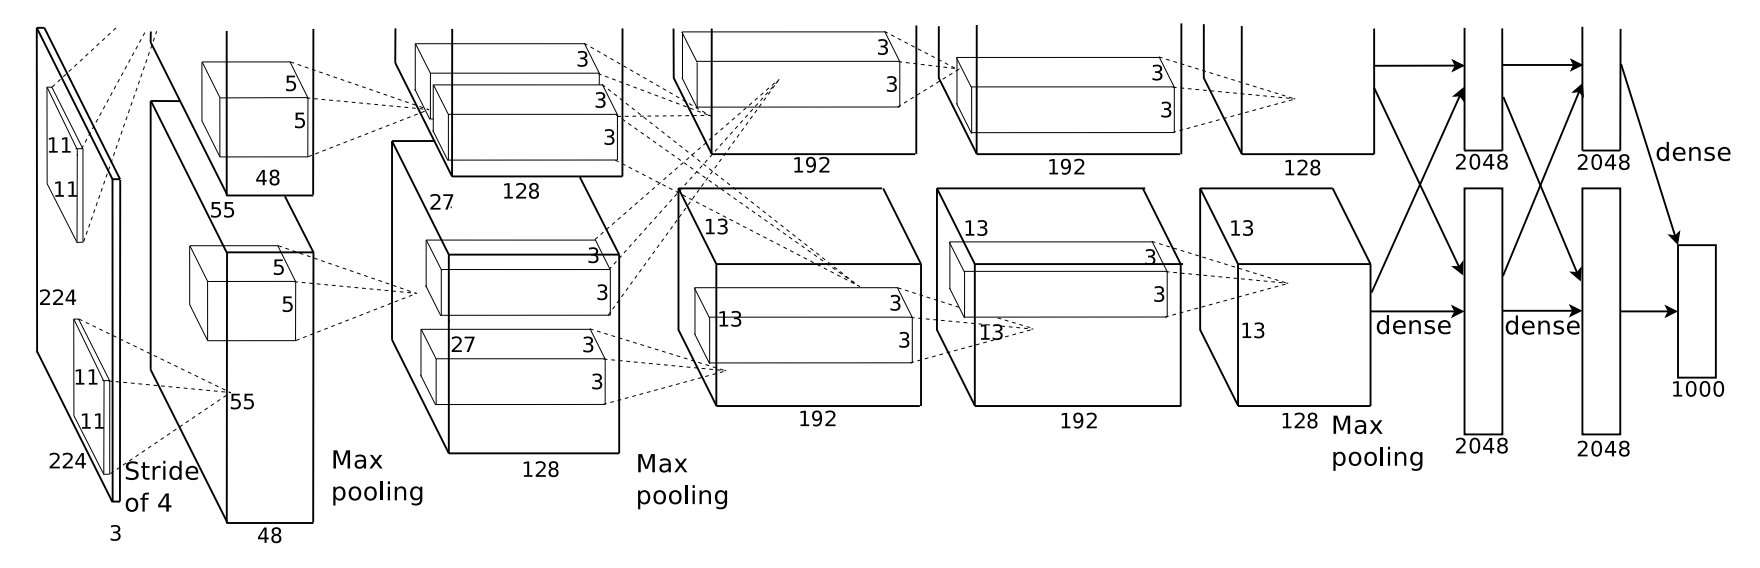
\includegraphics[width=\textwidth]{endoscopy_resources/alexnet.png}
    \caption{Architecture of AlexNet.  \cite{AlexNet}}
    \label{fig:alexnet_arch}
\end{figure}

\subsection{GoogLeNet / Inception} 
The GoogLeNet \cite{inception} was introduced in 2014, it consists of 22 layers together with the Inception Module which described in Figure \ref{fig:inception_block}. Inspired by the fact that salient parts inside an image can have extremely large variation in size and as a result, it is very difficult to choose the right convolution kernel. Because of this, convolution kernels at multiple scales: $1\times1 conv$, $3\times3 conv$, $5\times5 conv$ are done altogether for the previous input, and stack together again at output. The goal of the $1\times1  conv$ is reducing the dimensions of features space. Different kinds of features are extracted because multiple scale of convolutions as well as max pooling are tried simultaneously. Popular versions of InceptionNet includes: Inception v1 \cite{GoogleLeNet}, Inception v2 and  Inception v3 \cite{InceptionV2}, Inception v4 and Inception-ResNet \cite{InceptionV4}.
\begin{figure}[thb]
    \centering
    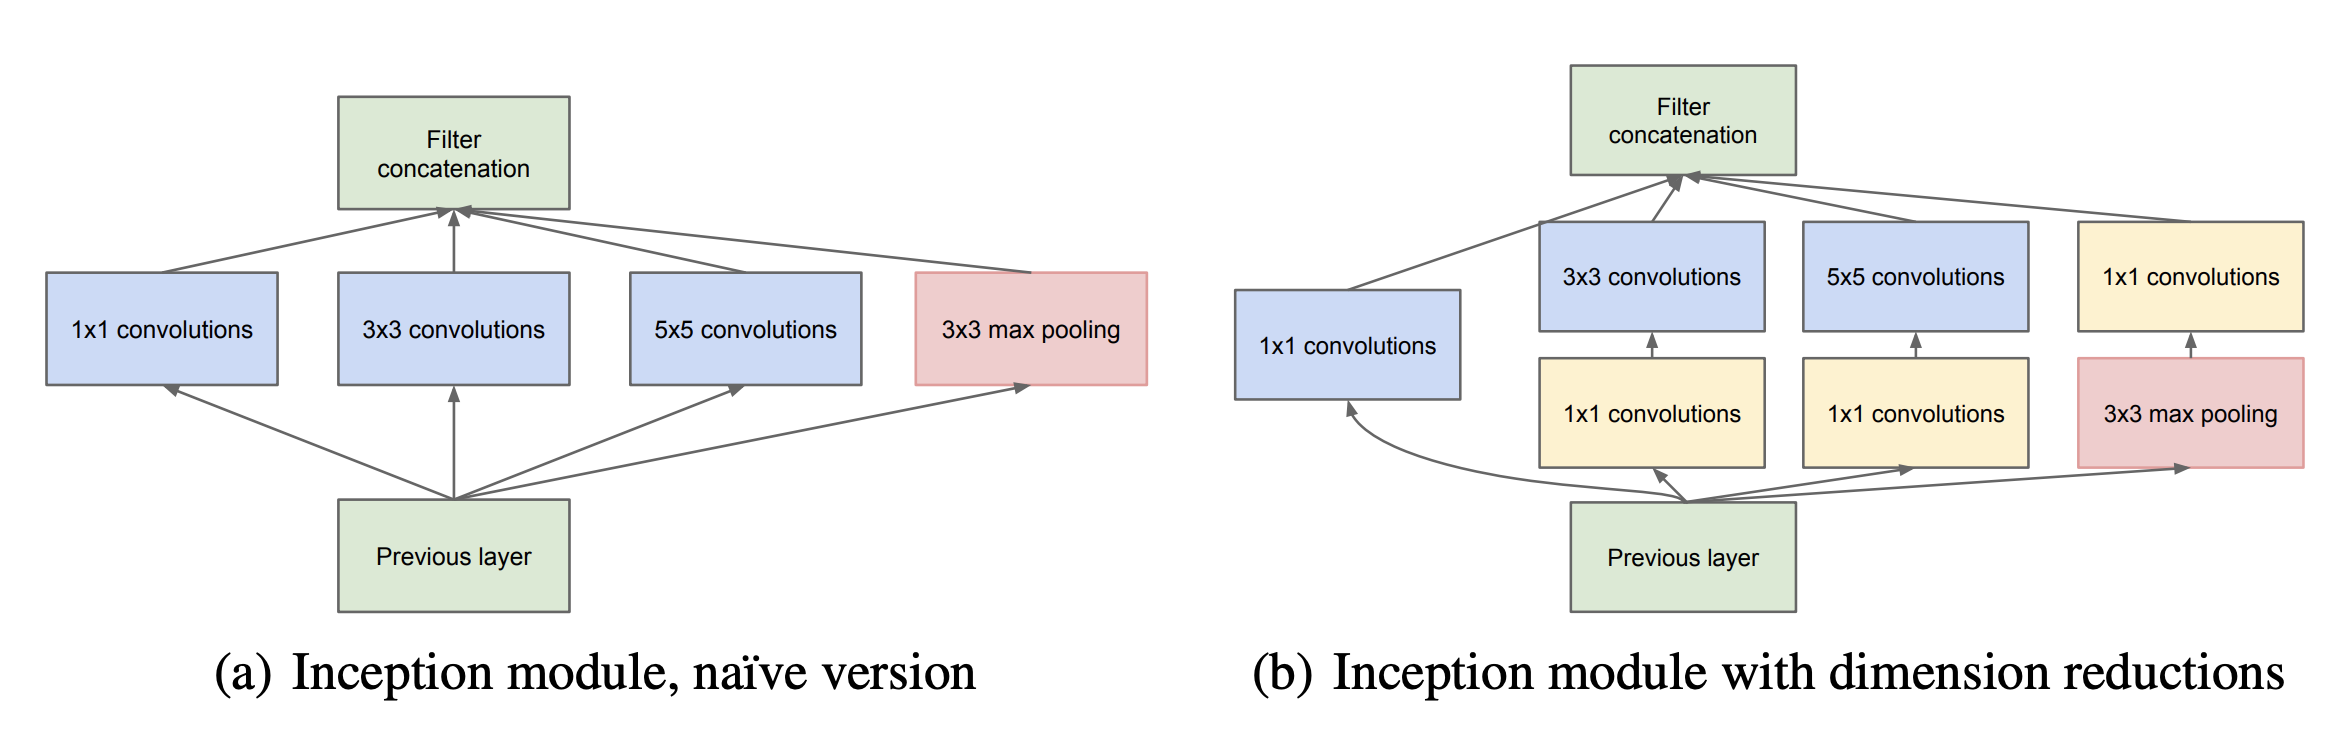
\includegraphics[width=\textwidth]{endoscopy_resources/inceptionnet.png}
    \caption{Inception block. \cite{inception}}
    \label{fig:inception_block}
\end{figure}

\subsection{Residual Neural Network (ResNet)}
In 2015, He et al. introduced the first Residual Neural Network \cite{Resnet} architecture that apply shortcut connections in some layers. Image of a Single Residual Block is given in Figure \ref{fig:single_res}. Different with traditional neural networks where each layer is fed into the next layer consequently, residual blocks can not only feed into the next layer but also into the layers that 2-3 hops away. Thanks to its special design, ResNet allows the flow of memory or information from the initial layers to the last and solving a part of degradation problem that usually happened with deep learning models. ResNet architecture can gain accuracy from considerably increased depth, up to 152 layers. Different architectures of ResNet which are common used in practice are shown in Figure \ref{fig:resnet_arch}.

\begin{figure}[thb]
	\centering 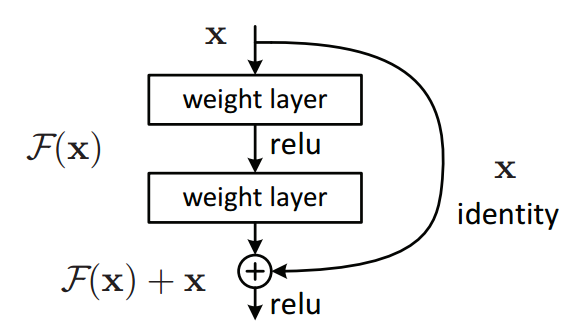
\includegraphics[width=0.5\columnwidth]{endoscopy_resources/single_residual_block.png}
	\caption[Single Residual Block.]{Single Residual Block.\footnotemark.}
	\label{fig:single_res}
\end{figure}
\footnotetext{\url{www.towardsdatascience.com}}

\begin{table}[thb]
    \centering
    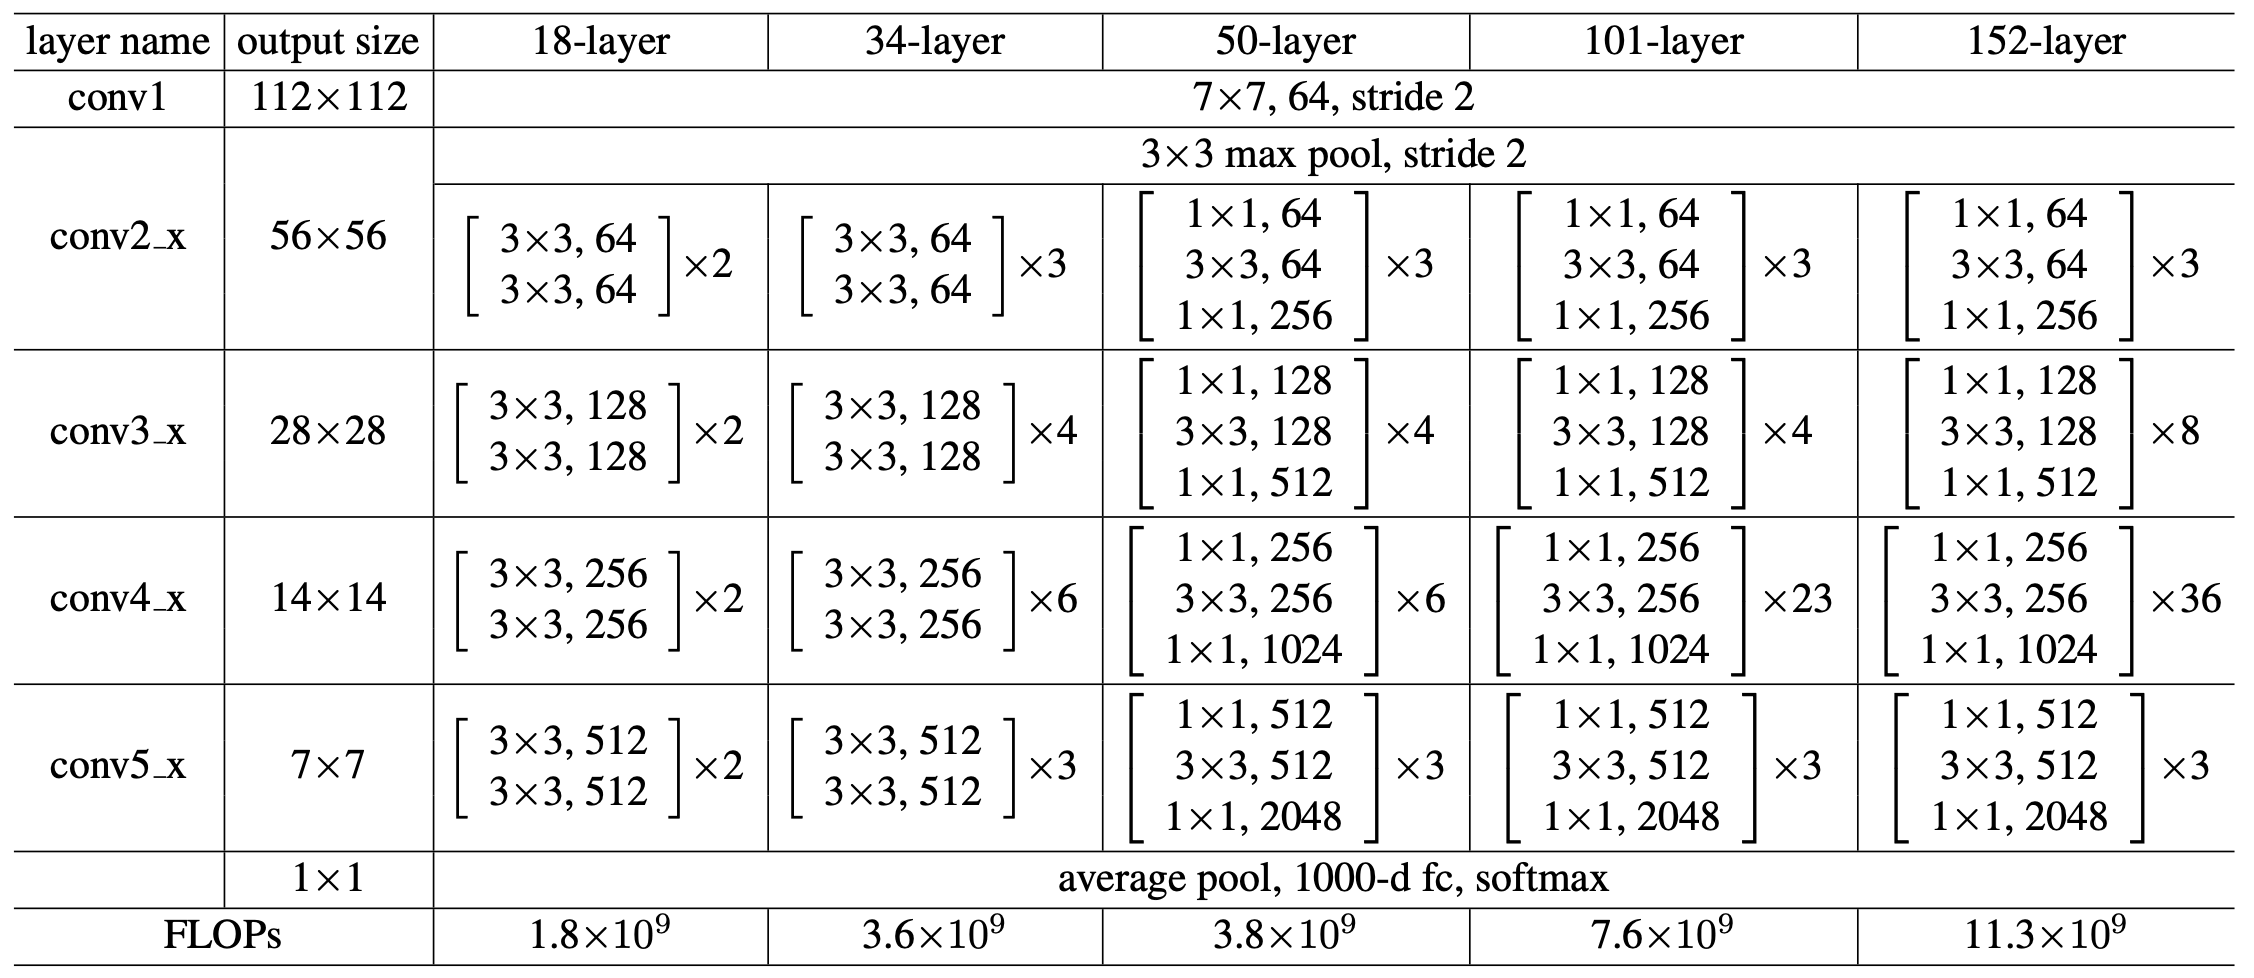
\includegraphics[width=\textwidth]{endoscopy_resources/resnet_archi.png}
    \caption{Different architectures of ResNet. Residual blocks are shown in brackets. \cite{Resnet}}
    \label{fig:resnet_arch}
\end{table}

\subsection{DenseNet}
In other to strengthen features propagation and alleviate the vanishing-gradient, DenseNet \cite{DenseNet} was introduced in 2017 that each layer takes all preceding feature-maps as input and its own feature-maps are used as inputs into all subsequent layers. Figure \ref{fig:dense_net} illustrates a 5-layer dense block with a growth rate of $k = 4$.
\begin{figure}[thb]
    \centering
    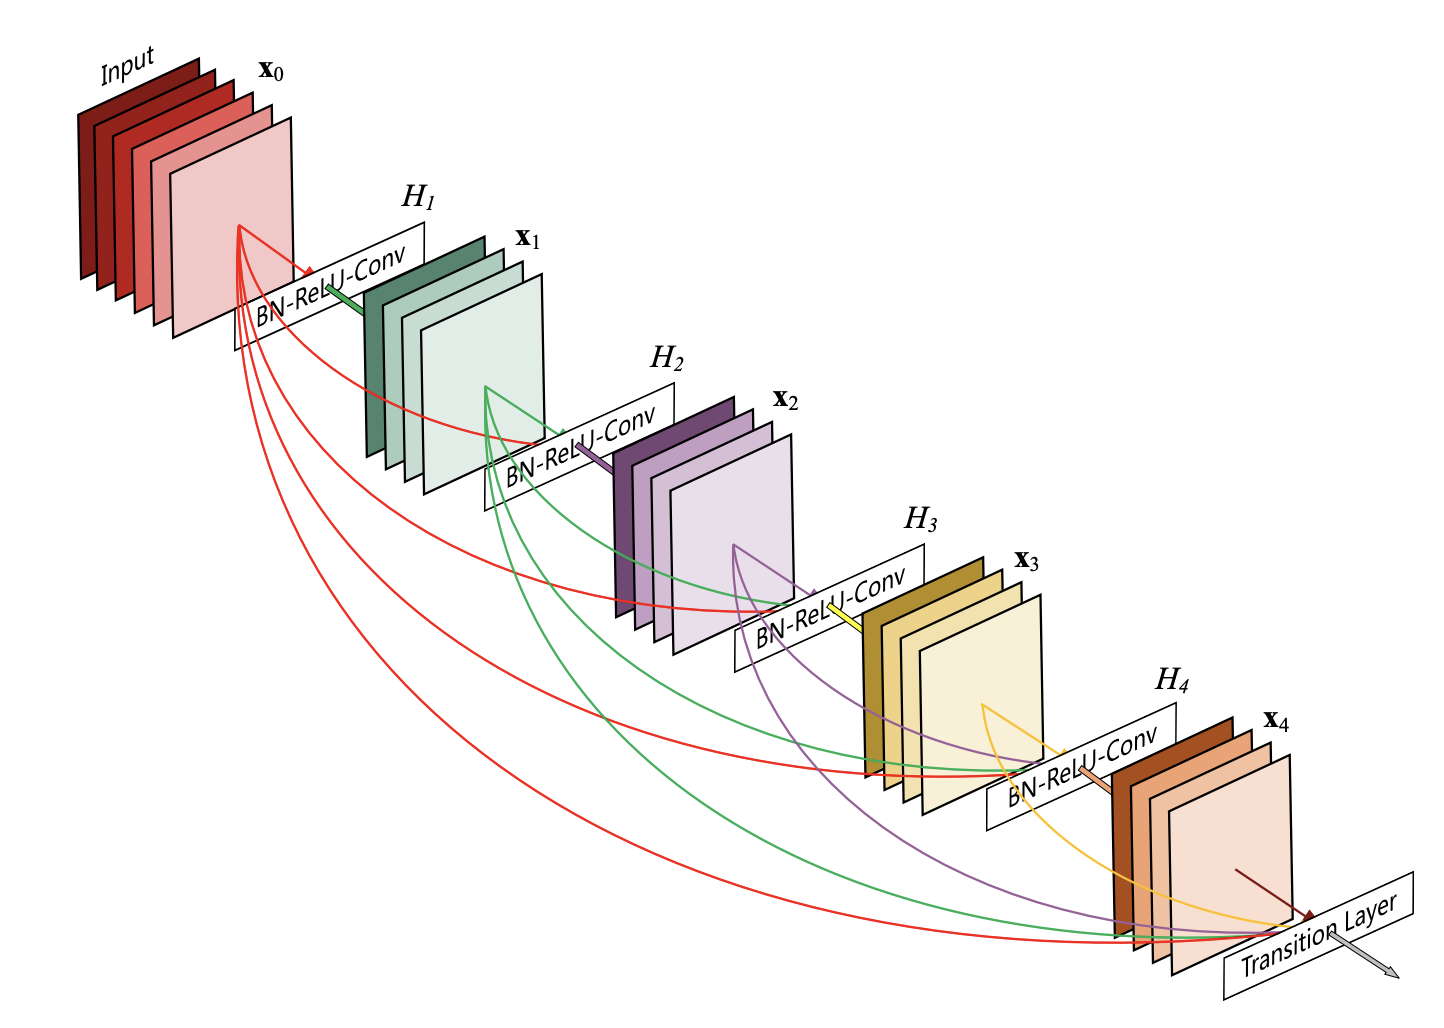
\includegraphics[width=\textwidth]{endoscopy_resources/densenet.png}
    \caption{A 5-layer dense block. \cite{DenseNet}}
    \label{fig:dense_net}
\end{figure}

\section{Object Detection}
Recognizing all objects with a given set of classes is one of the challenge in Computer Vision with a lot of approaches achieving high accuracy, such as Single-Shot Multibox Detector \cite{SSD}, Fast R-CNN \cite{FastRCNN}, Faster R-CNN \cite{FasterRCNN}, YOLO \cite{YOLO}, YOLOv2 \cite{YOLOv2}, YOLOv3 \cite{YOLOv3}. However, in the context of this work, we deiced to investigate and utilize the Faster R-CNN architecture.
\subsection{YOLO}
You Only Look Once (YOLO) \cite{YOLO} is an unified single-scale object detector that allows end-to-end training and real-time speed detection while maintaining high average precision. Introduced in 2016, the idea of YOLO is that a given input image can be divided into an $S \times S$  grid. For each cell in the grid, $B$ bounding boxes, confidence score for each box and $C$ class probabilities are predicted by the model. Figure \ref{fig:yolo_arch} shows the model of YOLO. A number of improvements are conducted on YOLO and put into practice as different versions i.e YOLOv2 \cite{YOLOv2}, YOLOv3 \cite{YOLOv3}.
\begin{figure}[thb]
    \centering
    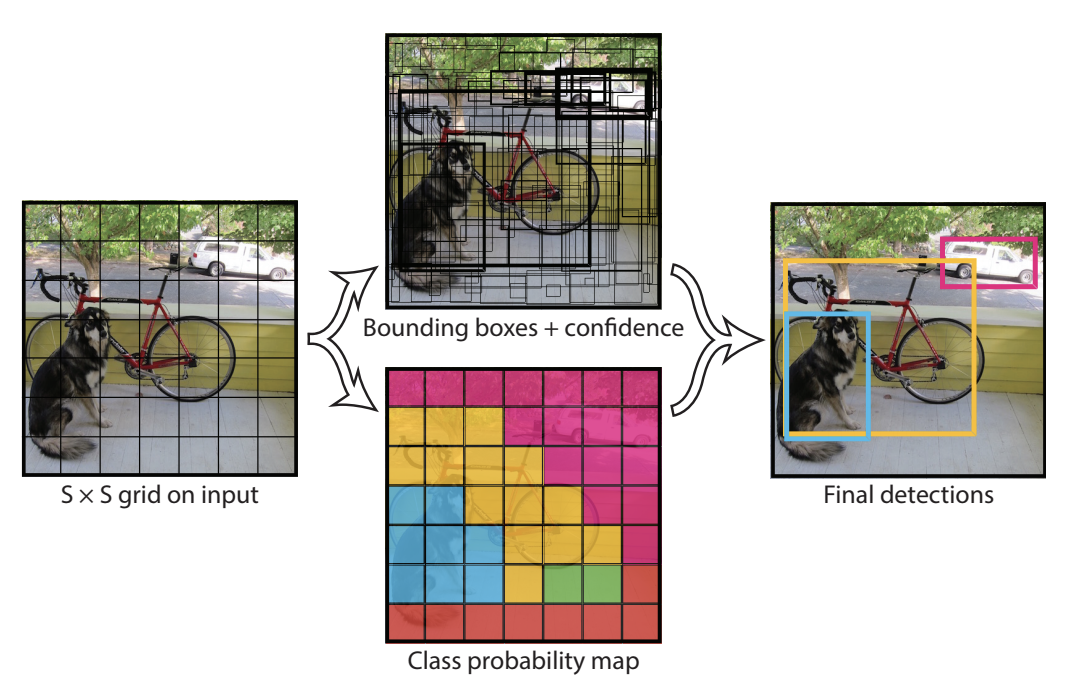
\includegraphics[width=0.7\textwidth]{endoscopy_resources/yolo.png}
    \caption{The model of YOLO \cite{YOLO}.}
    \label{fig:yolo_arch}
\end{figure}

\subsection{Faster R-CNN}
In general, both R-CNN \cite{RCNN} and Fast R-CNN \cite{FastRCNN} share a same approach. Firstly, selective search (SS) \cite{Uijlings2013} is used to generate region proposals. Secondly, a CNN-based network is applied to classify objects and detect the corresponding bounding box in those proposals. However, another approach is conducted on Faster R-CNN \cite{FasterRCNN} which uses a CNN architecture called Regional Proposal Network (RPN) instead of SS. Especially, this CNN is also shared with detection network and the average inference time is then reduced. Thus, the overall network is illustrated in Figure \ref{fig:frcnn_arch}.

\begin{figure}[thb]
    \centering
    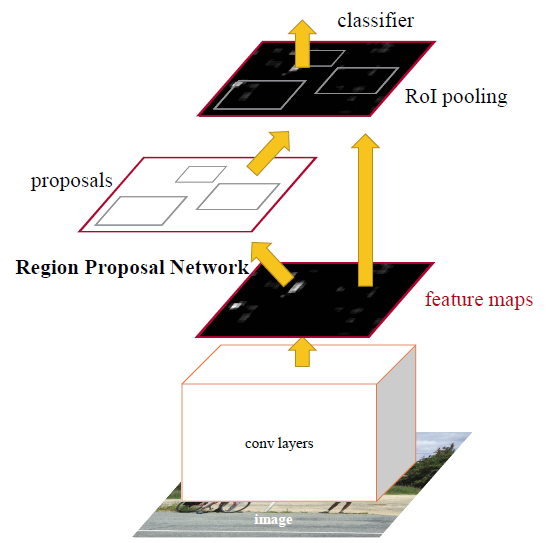
\includegraphics[width=0.7\textwidth]{endoscopy_resources/frcnn_arch.png}
    \caption{Faster R-CNN - a single, unifed network for object detection \cite{FasterRCNN}.}
    \label{fig:frcnn_arch}
\end{figure}

The pipeline of the RPN module of Faster R-CNN architecture is as follow:
\begin{figure}[thb]
    \centering
    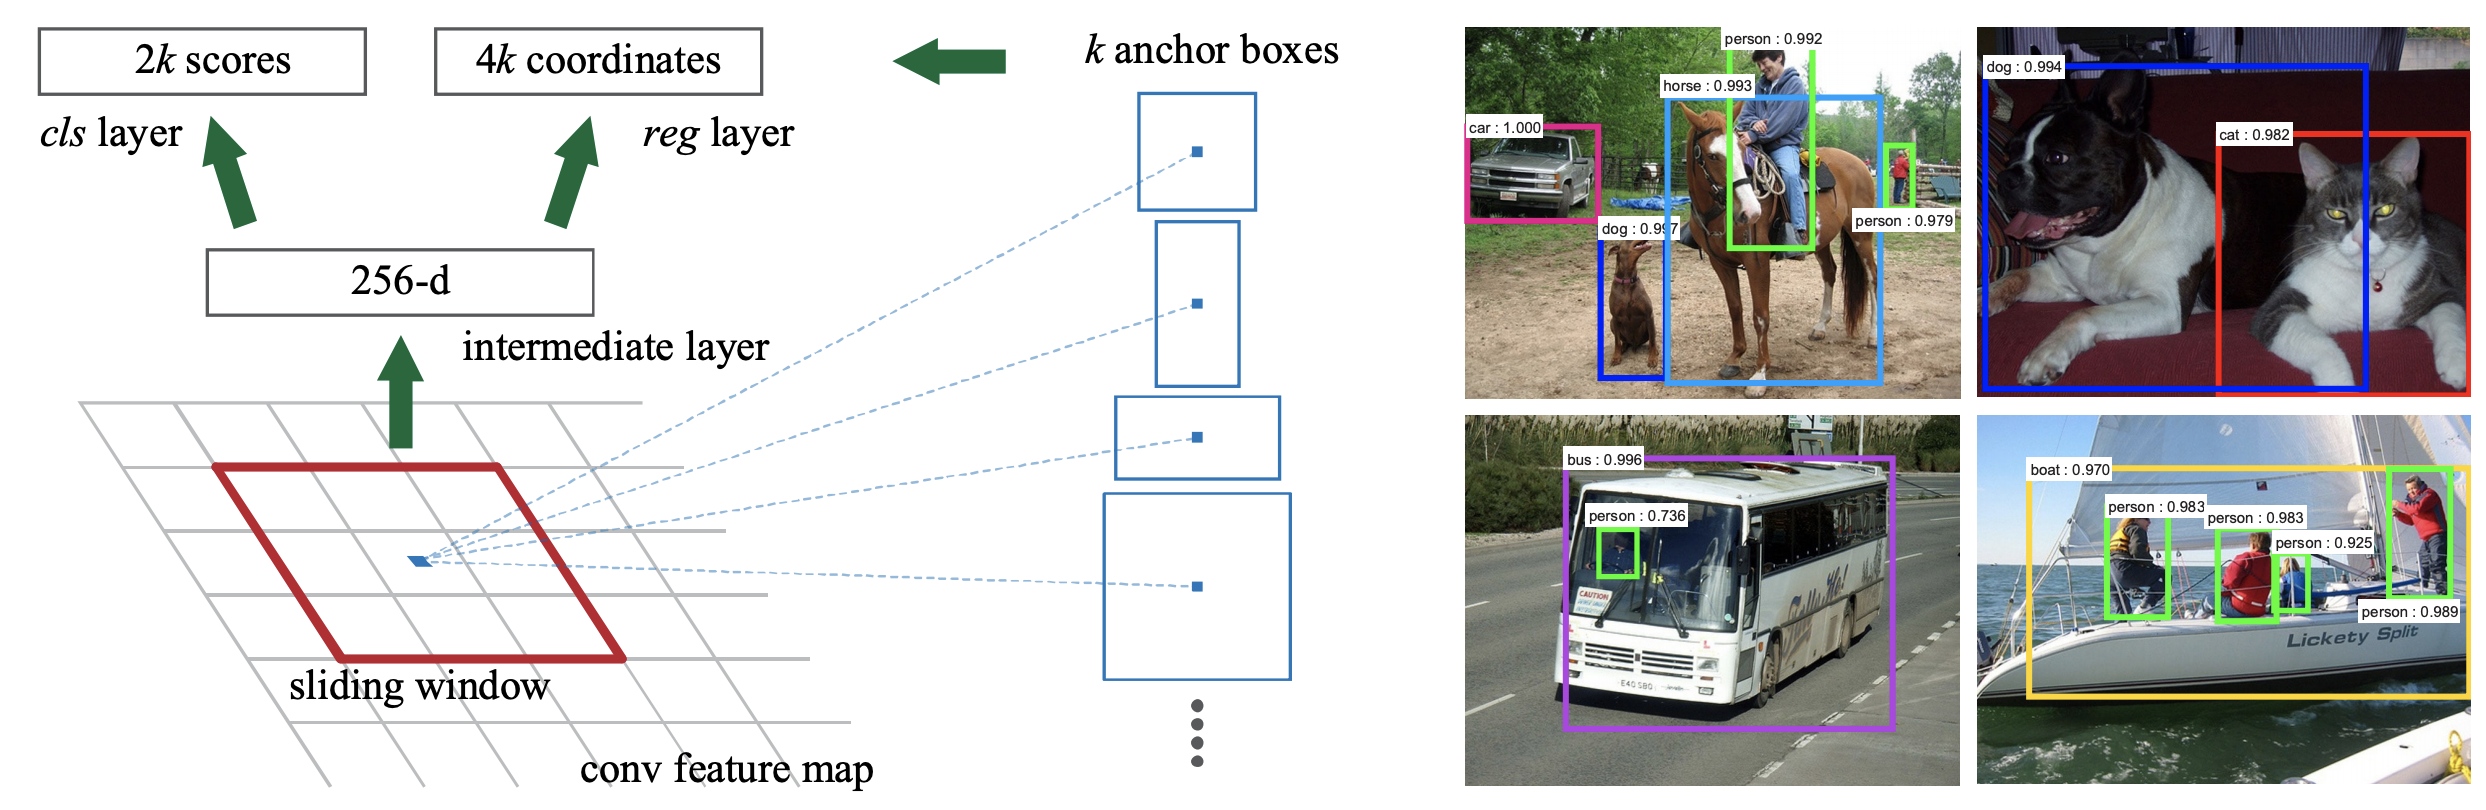
\includegraphics[width=0.9\textwidth]{endoscopy_resources/frcnn_rpn.png}
    \caption{Regional Propasal Network of Faster R-CNN (left) and example detections by using RPN proposals on PASCAL VOC 2007 (right) \cite{FasterRCNN}.}
    \label{fig:frcnn_rpn}
\end{figure}

\begin{itemize}
    \item The input image is inferred through deep convolution layers and features maps of its image are extracted.
    \item In the RPN module which is given in Figure \ref{fig:frcnn_rpn} (left), a sliding window is slidden over the features map. At each position, $k$ anchor boxes which have various scales and aspect ratios are used for generating region proposals.
    \item A $cls$ layer output $2k$ scores implies whether there is object or not for $k$ boxes, respectively.
    \item A $reg$ layer  output $4k$, regarding to the coordinate positions of $k$ boxes.
    \item Finally, all of the outputs are used to adjust the network to learn more accurate, the author defined the following loss function:
    \begin{equation}
        L(\{p_i\}, \{t_i\}) = \dfrac{1}{N_{cls}}\sum_{i} L_{cls}(p_i, p_i^{*}) + \lambda\dfrac{1}{N_{req}}\sum_{i}p_i^{*}L_{reg}(t_i, t_i^{*})
    \end{equation}
    It is noticeable that the above equation is the sum of two smaller loss function. The first part is the loss function for classification and the second part is for the regression. Here, $p_i$ and $t_i$ stand for the output of two layers of RPN, respectively. $p_i^{*}$ and $t_i^{*}$ are the ground-truth labels regarding to whether the given anchor is positive or negative (contains object or not) and the corresponding box is associated with a positive anchor.
\end{itemize}

Except the differences in the RPN module which is described above, the remaining part of Faster R-CNN is similar to the Fast R-CNN \cite{FastRCNN}. Consequently, after performing the ROI Pooling, the pooled area goes through CNN and two Fully Connected branches for class softmax and bounding box regression.

\subsection{RetinaNet}
Different with Faster R-CNN which is a two-stage detector, the RetinaNet  \cite{Retina} is a one-stage network architecture uses a Feature Pyramid Network (FPN) \cite{FPN} backbone on top of a feed forward ResNet architecture. The performance of both YOLO and Faster R-CNN mention above relies on choosing the right anchor size for each training dataset. Outcomes of RetinaNet compared to them is that it is possible to solve the multi-scale problems and generate a rich, multi-scale convolutional feature pyramid which can be further fed to sub-networks like classifying anchor boxes regressing anchor boxes to ground-truth object boxes. Despite having a simple design, the network proved to be surpassing all existing state-of-the-art two-stage detectors and still have a fewer inference time. The RetinaNet architecture is illustrated in Figure \ref{fig:retina_arch}.

\begin{figure}[thb]
    \centering
    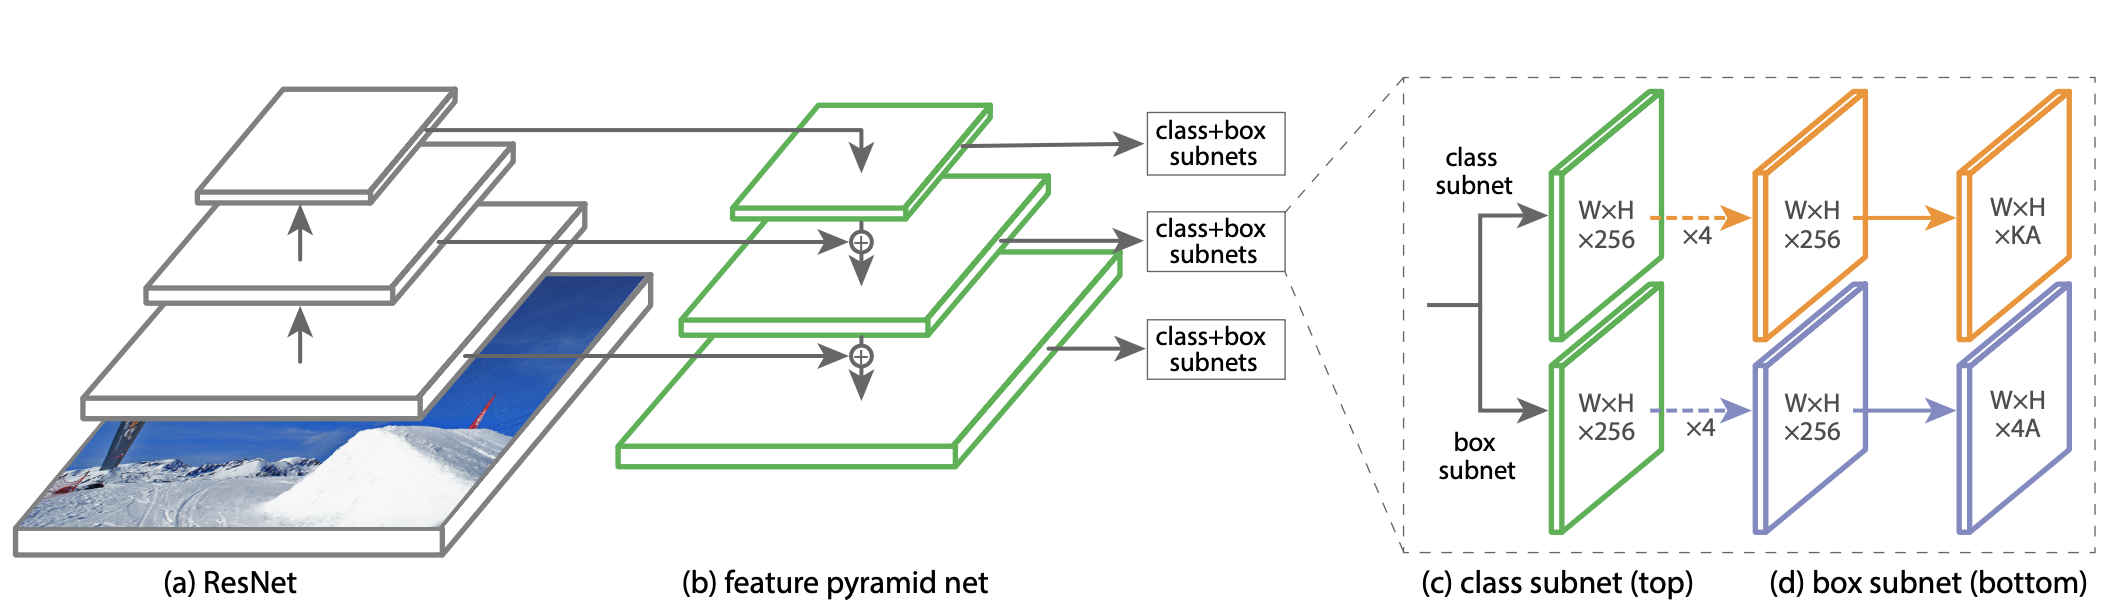
\includegraphics[width=\textwidth]{endoscopy_resources/retinanet.png}
    \caption{The RetinaNet architecture.\cite{Retina}}
    \label{fig:retina_arch}
\end{figure}
\section{Multimedia Assisted Diagnosis Systems}
The detection of abnormalities and diseases in early stages can significantly improve the chance of successful treatment and survival for patients. Multimedia community together with computer scientists can help medical doctors to improve the healthcare system through the application of their knowledge and methods to reach the next level of computer and multimedia assisted diagnosis. In details, these applications can solve a number of difficulties in processing images taking from medical devices. There is a need for an automatic assisted diagnosis system that can process, analysis, and retrieval on medical image and video. The key of these system is how to extract and integrate medical knowledge of experts on analyzing information from medical sensors with high accuracy and require as less as training data as possible. An example of such system is the EIR that conducted during the work of Michael et al. \cite{teammates} and illustrated in Figure \ref{fig:eir_system}. This system supports endoscopists in  the
detection and interpretation of diseases in the entire GI tract.
\begin{figure}[thb]
    \centering
    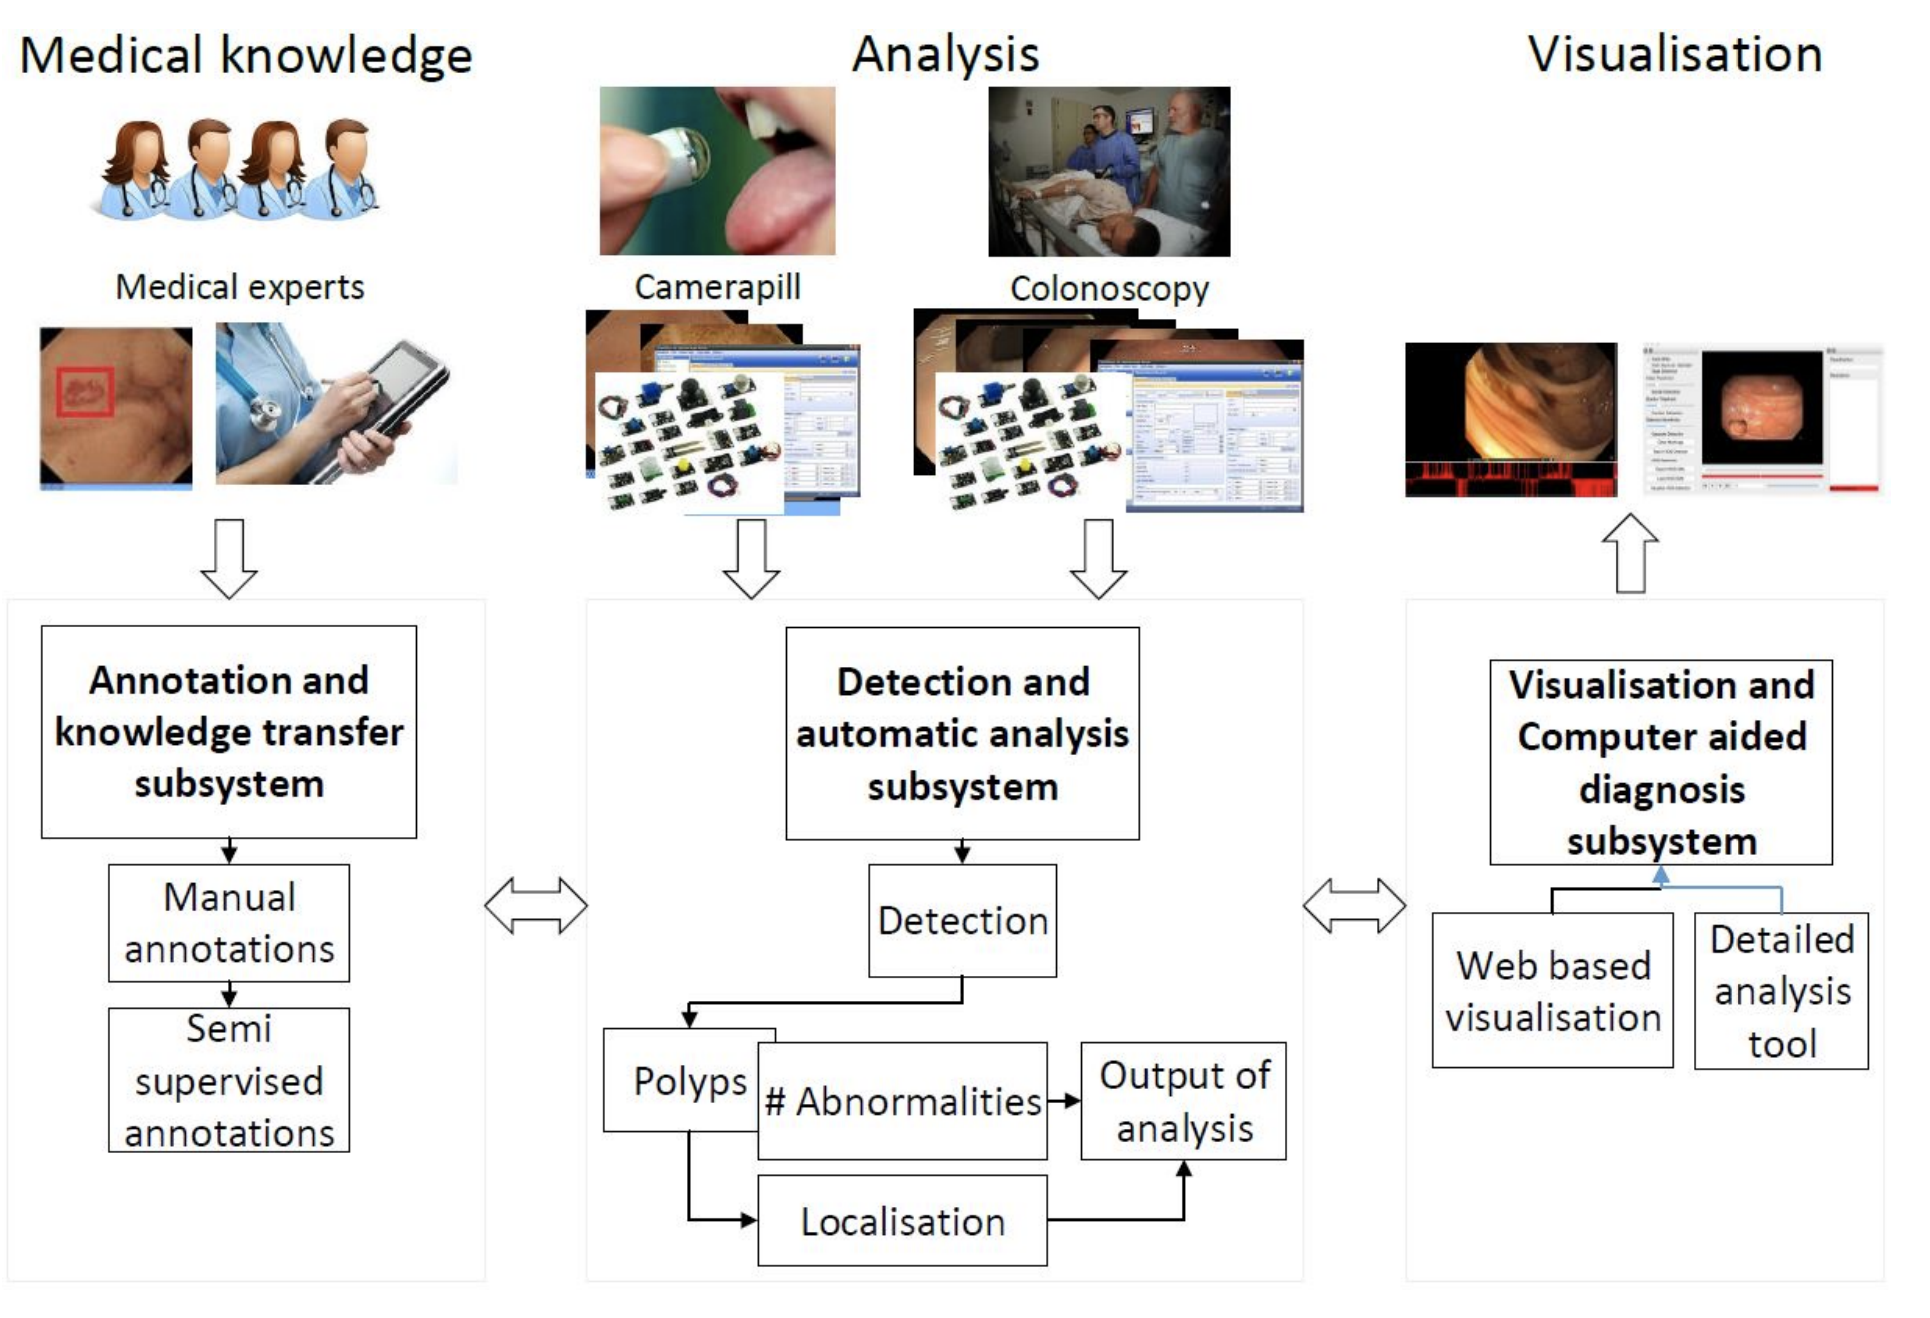
\includegraphics[width=0.9\textwidth]{endoscopy_resources/eir_system.png}
    \caption{EIR system: annotation and knowledge transfer, detection and automatic analysis and computer aided diagnosis.}
    \label{fig:eir_system}
\end{figure}

Beside  endoscopy examination, there are various field in medical diagnosis that can benefit. Most of the works conducted took the newest achievements of Convolutional Neural Network (CNNs). In Cardiac, Chest and Abdominal diagnosis, Tanno et al. \cite{Tanno} proposes a real time classification for vein compressibility analysis from Ultrasound signal. In order to build a system that can classify skin lesion automatically, Zhang et al. \cite{Zhang} has successfully introduced a system that apply deep learning model to overcome intra-class variation and inter-class similarity of skin lesions. Meanwhile, ultrasound images have been successfully classified and tumor malignancy can be detected automatically with CNNs network by the work of Liu et al. \cite{10.1007/978-3-030-00934-2_96}. Nevertheless, the results of this research showed that CNN classifier can not only perform a reasonable performance in predicting breast cancer, but also localize potential lesion regions which can be integrated into the breast ultrasound system in the future.

% Tackling the challenge can for example be addressed by leveraging techniques from multiple multimedia-related disciplines, including methods such as machine learning (classification), multimedia content analysis and multimodal fusion.

\section{Approaches in Endoscopic Images Analysis}
\subsection{Color space and handcrafted features approaches}
Early approaches that tackle with endoscopic image analysis usually work on the bleeding detection problem. Obviously, a bloody region usually has salient color which is significant different from other background areas. A simple approach is using color threshold and applying some handcrafted features in order to localize bleeding symptoms. Shah et al.\cite{HSIColorDomain} and Jung et al.\cite{active_blood_detect} proposed several solutions using color domain and region segmentation. Meanwhile, Novozamsky et al. \cite{blood_detection_color} proposed two technique in counting the number of pixels and localization of bloody region. The first one is defining color spaces that provides good separability of blood pixels. The second is based on an assumption about the shape and size of blood spot and use edge detectors.
Intermediate steps of the second technique are given  
in Figure \ref{fig:blood_detect_color}.

\begin{figure}[thb]
    \centering
    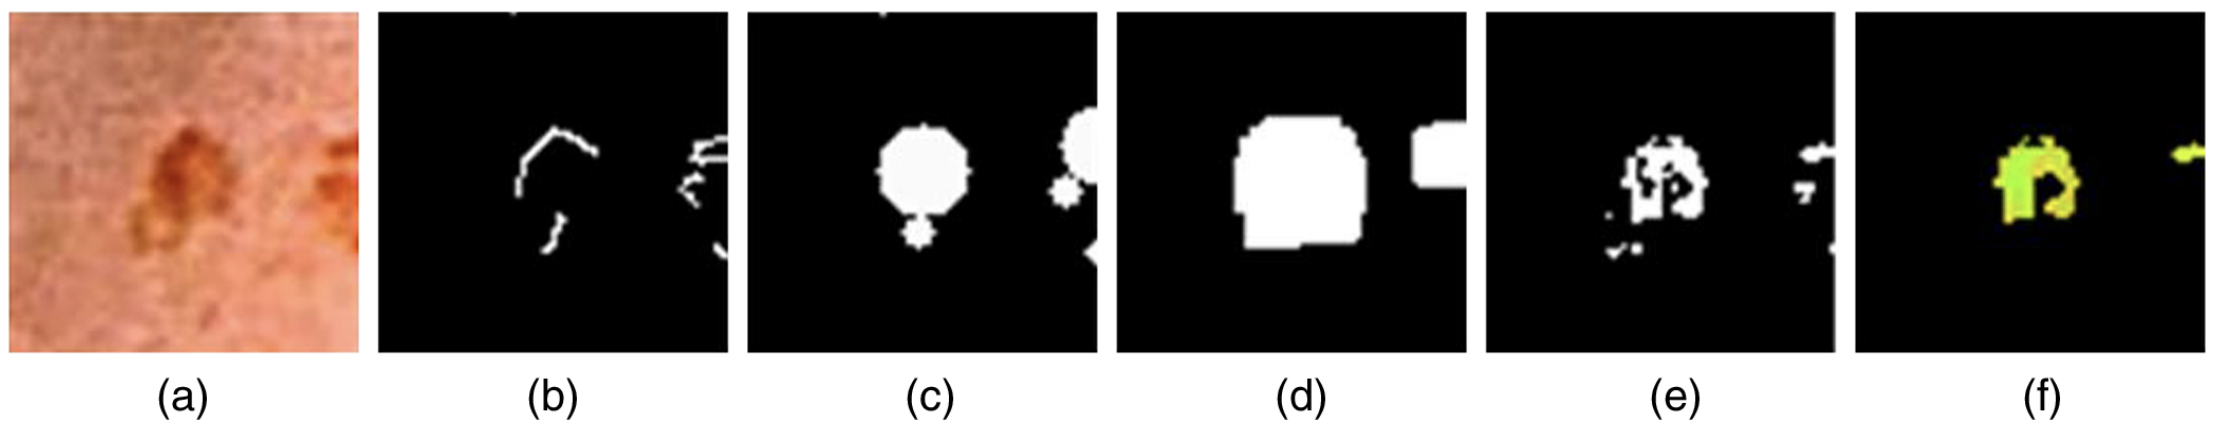
\includegraphics[width=\textwidth]{endoscopy_resources/blood_color.png}
    \caption{Blood detection with the second method.  (a) Input image. (b) Output of Canny detector. (c) Approximate closed-boundary regions. (d) Morphological operation. (e) At the same time, the input image (a) is converted to HSV and potential blood pixels are masked. (f) The output created by intersection of (d) and (e).\cite{blood_detection_color}}
    \label{fig:blood_detect_color}
\end{figure}


\subsection{Machine learning approaches}
Iakovidis et al. \cite{bloodsalientsuperpixels} proposed a solution to detect blood inside endoscopic images which based on a definition of superpixel saliency. Using the information about their color, the
saliency of superpixels is assessed and
enabling the identification of image regions that are likely to contain blood. The blood patterns are recognized by their color features using a supervised learning machine. Proposed solution is illustrated in Figure \ref{fig:super_pixel} through the visualizations of each step.
\begin{figure}[thb]
    \centering
    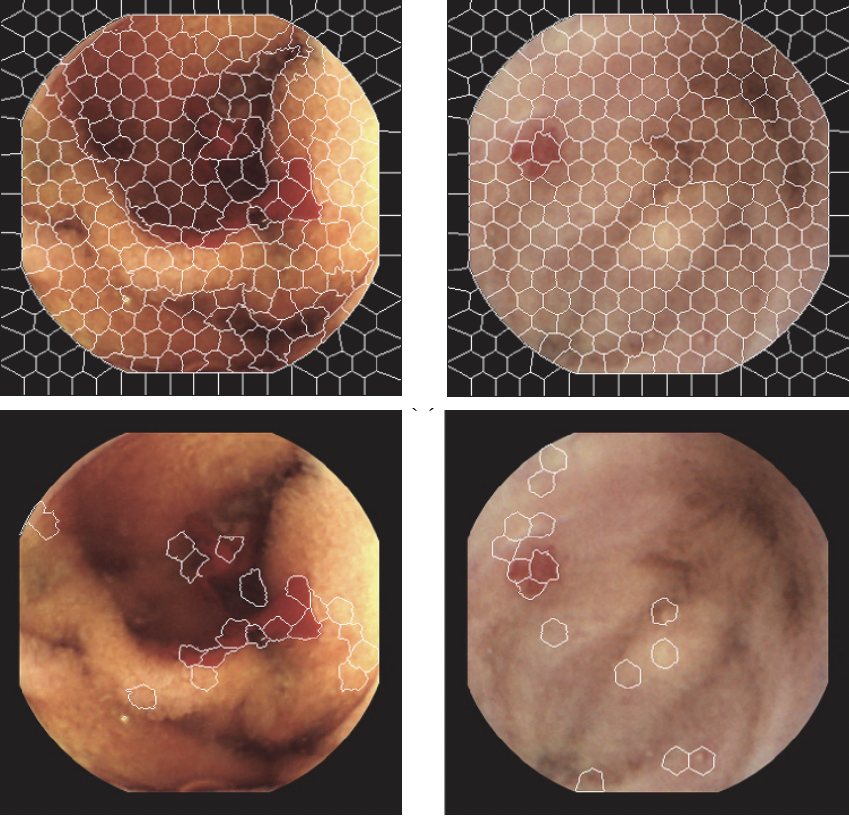
\includegraphics[width=0.6\textwidth]{endoscopy_resources/super_pixels_salient.png}
    \caption{Endoscopic blood detection based on Salient Super pixels.\cite{bloodsalientsuperpixels}}
    \label{fig:super_pixel}
\end{figure}
\subsection{Deep-learning approaches}
In the field of medical image processing, deep neural networks has proved it advantages in order to solve several problems related to endoscopic images of the human gastrointestinal (GI) tract. Particularly, to localize and identify polyps within real-time constraint, deep CNNs has recently shown an impressive potential when achieving up to 96.4\% accuracy - published in 2018 by Urban G et al. \cite{urban_tripathi_alkayali_mittal_jalali_karnes_baldi_2018}. Another interesting article of Satoki Shichijo et al. \cite{Shichijo2017} also applies multiple deep CNNs to diagnose Helicobacter pylori gastritis based on endoscopic images. According to the research, after training with more than 30,000 endoscopic images, the accuracy of the CNNs is comparable to that of endoscopists. CNNs approaches is substantially shorter time and contribute to reducing the efforts of endoscopists. Further, gastrointestinal bleeding detection using deep CNNs on endoscopic images has been successfully done and published by Xiao Jia et al. \cite{jia_meng_2016} with impressive $F_1$ score up to 99.55\%. The CNNs architecture conducted in this research is shown in Figure \ref{fig:cnns_bleeding}.

\begin{figure}[thb]
    \centering
    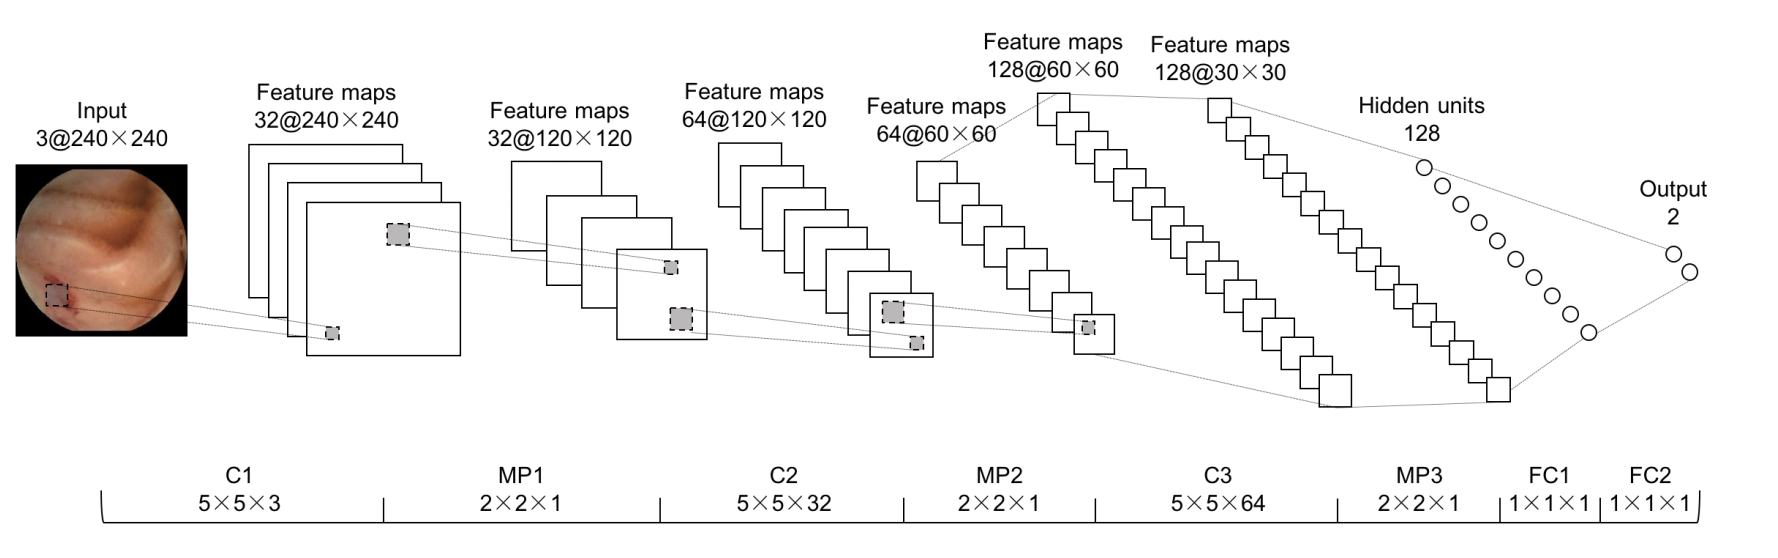
\includegraphics[width=\textwidth]{endoscopy_resources/cnns_bleeding_detection.png}
    \caption{Gastrointestinal bleeding detection CNNs architecture proposed by Xiao Jia et al.  \cite{jia_meng_2016}}
    \label{fig:cnns_bleeding}
\end{figure}

% \section{Dataset Augmentation}
% One of the biggest problem of Deep Neural Network is that it requires a large number of training samples. However, in some cases it is insufficient to have such amount of data. Applying several simple augmentation strategy like Random Flip, Random Rotation, Random Brightness and Contrast augmentation can also be applied. Novel approaches in data augmentation are taking into account where Another approach like using \cite{DBLP:journals/corr/KhorevaBIBS17}

\section{Image Segmentation}

Beside the object detection problem, image segmentation requires not only detected and classified bounding boxes around the interested objects but also the accurate contours of those ones. These results from image segmentation provide finer features about the segmented objects, such as size, shapes, orientation, etc, that can further be used to analyze the object's properties. There are two main degrees of solving this kind of problem: semantic segmentation and instance segmentation. The former are focusing on grouping the pixels in image into a semantically meaningful results, i.e. object category, while the latter requires a further instance separation step to make each instance in same object category distinctively. Figure \ref{fig:3_object_vs_instance} visualizes the desired results of each type of problems, including semantic segmentation and instance segmentation.

\begin{figure}[thb]
    \centering
    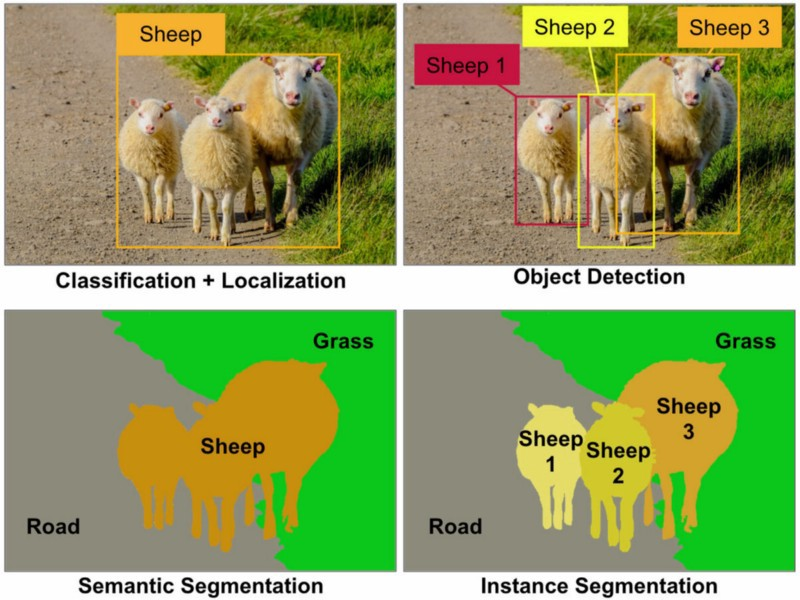
\includegraphics[width=\textwidth]{resources/3_object_vs_instance.jpeg}
    \caption{Difference between desired results from different tasks in Computer Vision \cite{instace_vs_object}.}
    \label{fig:3_object_vs_instance}
\end{figure}

Well-known approaches before deep learning often exploit the relationship of color, intensity or texture of region around the interested pixel. K-means clustering \cite{kmean} or other graph-based algorithms such as minimum spanning tree based segmentation (MST based segmentation), energy minimization using Graph Cuts \cite{FastGraphCuts, EfficientGraphBasedSegmentation}, GrabCut \cite{GrabCut}, etc. are often utilized to do region-based segmentation. However, some variations in the data, such as color, illumination, texture or non-rigid orientation, makes these approach difficult to generalize well in real-life conditions. 

Inheriting from recent achievement of deep learning in solving object detection problems, new neural network achitecture has been proposed to tackle the segmentation problems, in both semantic level and instance level. PASCAL VOC \cite{PASCALVOCDataset} and MSCOCO \cite{MSCOCODataset} become standardized datasets for the segmentation problems. Many recent proposed methods try to beat the state-of-the-art on these datasets, however, most of them share a basic underlying designed architecture which is known as Fully Convolutional Networks (FCNs) \cite{FCNs}. This is a typical networks for semantic segmentation by replacing the last fully connected layers of object detection network by a decoder network which restores the original resolution of input image by using transposed convolutional layers which are may known as deconvolutional layers. In more details, the network must consist of two main stages: Encoder stage which converts image in original pixel space to a learned feature space and Decoder stage which maps the extracted features to the result space, which often has same dimension as the original input image. An example of this process is illustrated in Figure \ref{fig:CL_DL}. DeepLab \cite{DeepLabv1,DeepLabv2,DeepLabv3,DeepLabv3+}, Pyramid Scene Parsing Net \cite{PSPNet} for semantic segmentation or Mask R-CNN \cite{MaskRCNN} and MaskLab \cite{MaskLab} for instance segmentation are well-known approaches lately designed based on this architecture.

\begin{figure}[thb]
\centering
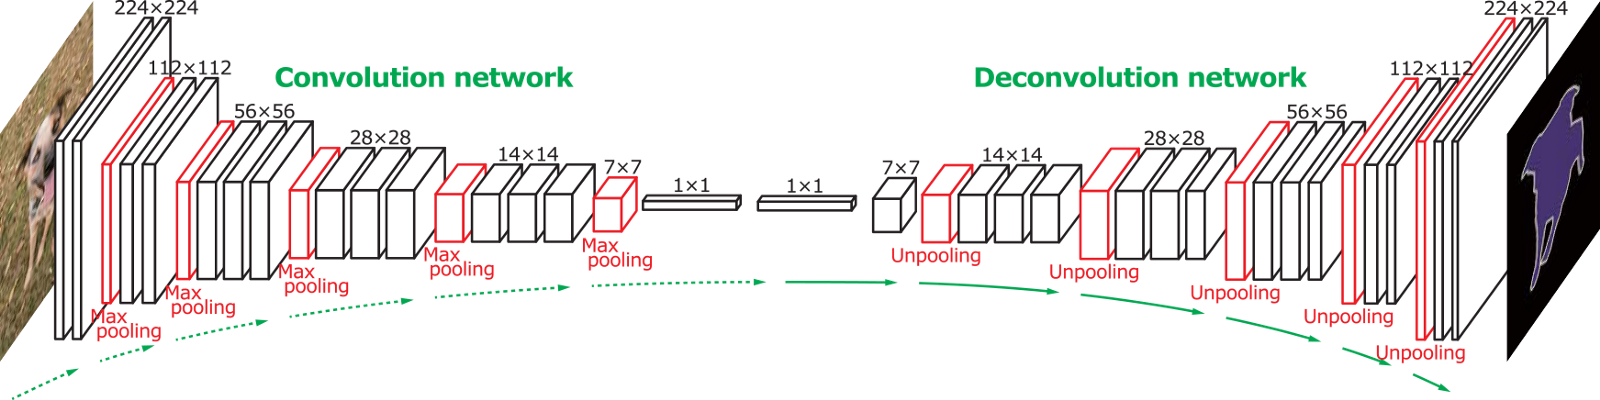
\includegraphics[width=1\textwidth]{resources/3-conv-deconv.png}
\caption{Two stages of FCNs: Encoder process with convolution network and decoder process with deconvolution network \cite{conv_deconv}.}
\label{fig:CL_DL}
\end{figure}

U-Net \cite{unet} shares some similarity in the network design with FCNs \cite{FCNs}; however, the long skip connections are included to connect the features from encoder branch to the decoder branch. The authors argues that the features from encoder stages containing low-level features such as edges, contours, etc. that needs to be preserved during the decoder stages. To achieve this property, features from encoder layers at the same level could be simply copied and concatenated with the deconvolved results, then go through a convolutional layers, yielding a combined features between encoder and decoder branch. These features, as described in the U-Net paper \cite{unet}, contain discriminative property that can help pixels, especially pixels on boundary, to have better classification results. Figure \ref{fig:u_net} visualizes the design of a typical U-Net architecture.

\begin{figure}[thb]
    \centering
    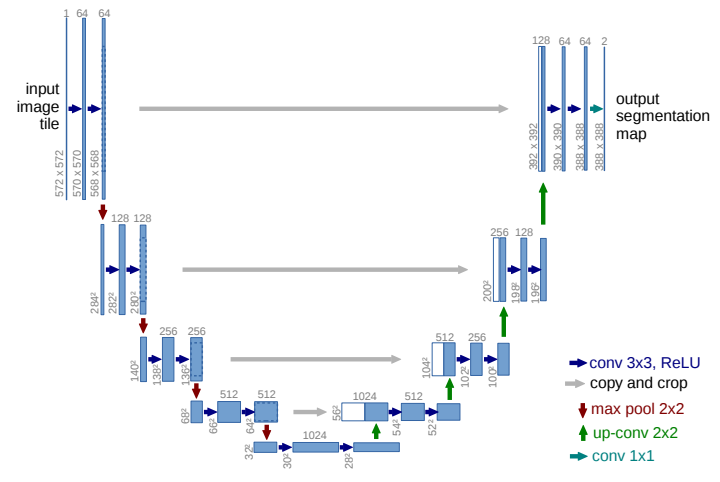
\includegraphics[width=\textwidth]{resources/3_u_net.png}
    \caption{U-Net architecture \cite{unet}.}
    \label{fig:u_net}
\end{figure}

\section{Nuclear segmentation in Medical Image Analysis}

In this section, we review approaches used to solve segmentation problems in medical image analysis. These methods are grouped in each subsections to better describe the merit of each family solution. Most of materials in this section are referenced from these comprehensive reviews \cite{review_seg_overall}, \cite{survey_on_medical_image_analysis}. 

\subsection{Intensity thresholding}
This could be the first and simplest method for nuclear segmentation. Based on the sufficient and consistent distinction of the intensity distributions between nuclei/cells and the background, the Otsu’s method \cite{Otsu} performs statistical discriminant analysis of the image intensity histograms, and chooses an optimal threshold value by maximizing the interclass variance. To deal with the noise or nonuniform illumination, image is divided into sub-images to perform local thresholding. This requires an additional parameter, which is the local region size, needed to tune during developing the algorithm. Some proposed methods use the merit of intensity thresholding to separate the nuclei from background such as Callau \textit{et al.} \cite{Callau2015} for segmenting the epithelial cell areas in breast cancer TMA images, Keenan \textit{et al.} \cite{Keenan2000AnAM} for isolating nuceli in cervical images, etc. 

\begin{figure}[thb]
    \centering
    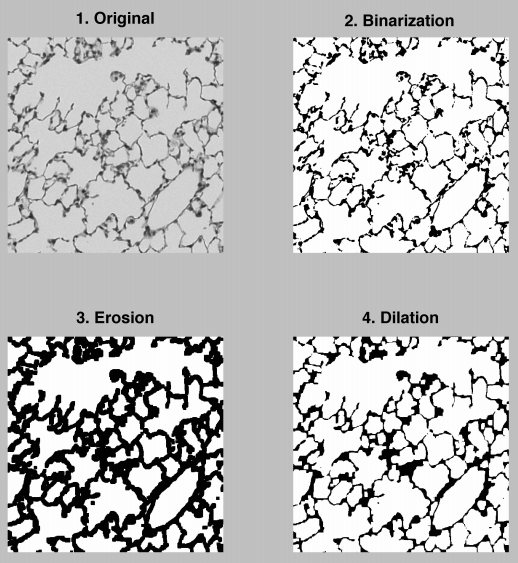
\includegraphics[width=0.5\textwidth]{resources/2_morphological_seg.png}
    \caption{Segmentation of lung patches using binarization, erosion and dilation operators. \cite{morphological_seg}}
    \label{fig:morphological_seg}
\end{figure}

\subsection{Morphology Operations}
By applying thresholding to binarize the input image, erosion and dilation, which are two basic morphology operations \cite{morphology1}, are used to create segmentation results. Iterative erosion operators with increasing scales are applied until obtaining the markers. These markers become cell seeds indicating regions of individual nuclear. Dilation are iteratively used to expand the cell seeds region, creating the final segmentation results. However, for dense cell clumps, this method oftens produce undersegmentation results. Figure \ref{fig:morphological_seg} visualizes the results of each step when morphology operations are applied to do segmentation task on medical images. 

\subsection{Watershed Transform}
In watershed transform \cite{watershed}, an image is viewed as a landscape which the intensity of pixels is considered as altitude. The algorithm starts at the local minima as independent seeds and iteratively adds the connected regions to merge them into nearest union components. In other ways, watershed transform floods the terrain by filling the water from the lowest point in local regions. The dams, which are call watershed lines, are built to prevent water from merging when water from distinct regions is going to meet. The procedure stops when  water reaches the highest point. The main drawback of this approach is that it produces excessive over-segmentation, especially for natural images. There are some works based on this typical idea such as Long \textit{et al.} \cite{long_watershed}, Yang \textit{et al.} \cite{yang_watershed}, etc.

\subsection{Clustering}
K-means clustering \cite{kmean} applied by Kothari et al. \cite{clustering1} to do segmentation in H\&E and IHC stained pathology images or Arif and Rajpoot \cite{clustering2} on nuceli segmentation. Other soft clustering algorithm, such as fuzzy c-mean (FCM) \cite{fuzy}, are also used in nuclei segmentation \cite{parallel_fuzy}. However, due to lack of nucleus shape prior, the cell seed need to be generated to create the number of original groups which lead to unreasonable boundary results. 

\subsection{Graph-based methods}
There are several approaches in the graph-based method to solve nuclear segmentation. Max-flow/min-cut \cite{maxflow} often try to minimize a defined energy function which can separate the nuclei from background. Another approach is normalized cut \cite{normalized_cut} which tries to recursively separate the graph into two disjoint set with a minimum cut. Conditional Random Field (CRF) \cite{crf} is a discriminative graphical model people also often use to do image segmentation. Wu et al. \cite{6157605} applies this idea to do segmentation in cytology images.

\subsection{Deep learning}

With the recent advances of deep learning on other related fields in Computer Vision such as object detection, as well as the increasing amount of training data in medical image analysis, there are a shifting attention of research community from previous mentioned approaches to deep learning. There are a lot of grand challenges in digital pathology, boosting the maturity of this research area. A lot of deep learning methods achieved the highest rank in these challenges, such as Ciresan \textit{et al.} \cite{NIPS2012_4741} in EM segmentation challenge 2012, Xu \textit{et al.} \cite{DBLP:journals/corr/XuLLWLC16} in GLAS for gland segmentation, etc. Ehteshami Bejnordi \textit{et al.} \cite{7243333} even outperform the performance of a pathologist on the test set of CAMELYON16 challenge for processing breast cancer tissue samples. The staining and imaging modality are also diverse, including hematoxylin and eosin staining (H\&E), tumor-infiltrating lymphocytes (TIL), electron microscopy (EM), fluorescent (FL), etc. This demonstrates a great potential of deep learning applied in medical image analysis, especially nuclear segmentation.

\begin{figure}[thb]
    \centering
    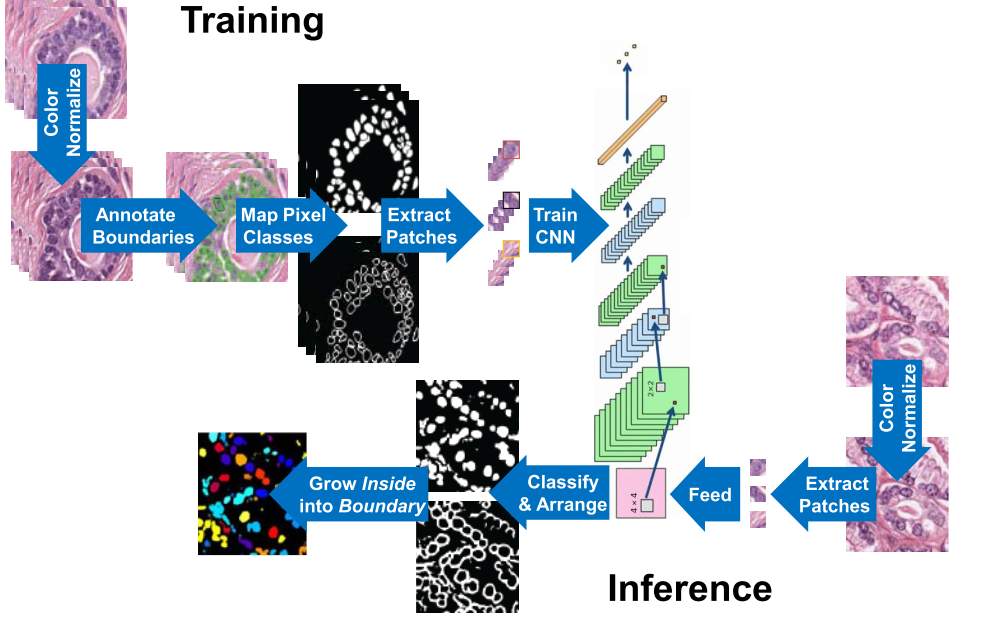
\includegraphics[width=\textwidth]{resources/3-cnn3.png}
    \caption{The proposed pipeline in CNN3 \cite{he_dataset_kumar} to do nuclear segmentation on H\&E stained histopathology images.}
    \label{fig:cnn3}
\end{figure}

One recent remarkable study by Kumar \textit{et al.} \cite{he_dataset_kumar} to perform nuclear segmentation on H\&E stained histopathology images attracts a lot of attention from research community. One of their main contribution is creating a new dataset containing 30 well-annotated images from TCGA project \cite{tcga}. As mentioned in \cite{he_dataset_kumar}, the data comes from 18 different hospitals, covers seven different organs including breast, liver, kidney, prostate, bladder, colon and stomach, both benign and diseased samples. This creates a benchmark for research community to develop nuclear segmentation techniques specially on H\&E stained histopathology images with diverse nuclear types. Besides the proposed dataset, authors in \cite{he_dataset_kumar} also designed an approach to solve the segmentation problems. For better separation touching nuclear, 3-class probability assignment by deep neural network, including inside, outside and boundary, has been proposed. This becomes one of the basic configuration followed by later algorithms. Figure \ref{fig:cnn3} visualizes the pipeline proposed in \cite{he_dataset_kumar} in more details. As the reported result, this approach \cite{he_dataset_kumar} improves the F1-score to about 83\% compared to 40\% of a configuration of Fiji's \cite{fiji} segmentation algorithm. 

\section{Group equivariance in neural network}

\subsection{Equivariant property}

\begin{figure}[thb]
    \centering
    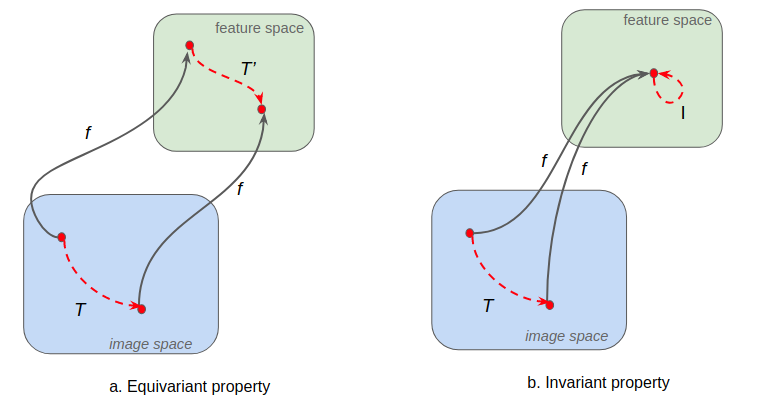
\includegraphics[width=\textwidth]{resources/2_equi_invar.png}
    \caption{Visualization of equivariance and invariance definition.}
    \label{fig:equi_and_invar}
\end{figure}


Let $f(x)$ is a representation of an input image x in the image space. This representation is equivariant to a family of transformations $I$ on image spaces if for any transformation $T \in I$, there exists a corresponding transformation $T'$ on feature spaces, such that

\begin{equation}
    f(Tx) = T'f(x)
\end{equation}

for any input images x \cite{dren}. It means that the representation of transformed input images are predictable if the transformation obeys the  equivariant rule. In case $T'$ equals to identity transformation, the representation remain unchanged no matter the transformed images as versions of input needed to be represented. This property is call invariant. A good classifier should owe this property to produce strong results under the dramatic change in the input space. Figure \ref{fig:equi_and_invar} visualizes the merit of each property including equivarance and invariance in an image space and its corresponding feature space. As proven in \cite{gcnn}, the convolutional neural networks are effective because of weight sharing mechanism, which activates the translation equivariance or translation invariance in most perception task. It means that the feature of shifted version of image feeded to the network is same as the shifted feature of the original images plugged to the same network. However, the features extracted from vanilla neural network cannot be equivariant to other group of transformation such as rotation, reflection, etc. It could be beneficial if these transformations could be cooperated to the network in the equivariant manners. For example, there is a family of special rotation transformations $R = \{R_{\theta} | \theta = k\pi/2, k \in Z \}$ that owns this equivariant property in the mathematics way. Encoding these group equivariance to the network yields the better generalization of the results produced by these architectures.


\subsection{Approaches}
Data augmentation is one way to force the network to learn equivariant/invariant feature representation. During the training process, some transformations could be applied on the input data to expand the input space the network has looked through. With enough capacity and huge amount of training data with defined set of transformations, the network could be able to force this property in its feature representation. However, the input space are often too huge to cover during the training process, there is no guarantee that the network could generalize the equivariant/invariant property outside the training set. Moreover, to learn this property, each parts of the network has to learn different representations of input data, for example different versions of rotation of input image. This sacrifies a lot of network capacity to learn these representation, which could be the duplicate of each others, instead of other useful features. Cooperating the equivariance/invariance to group of transformations could help the network generalizing better in the real-life scenarios.

Test time augmentation is often used to produce the results that are equivariant/invariant to transformations on the input data. For example, to obtain the equivariance/invariance property on the results created by CNNs, the multiple versions of input image are generated by a set of transformations. These images are then used to produce the predictions. The final result is the average ones of multiple transformed versions. This do not require to change any layers in the architecture design; however, it consumes a lot of computation resources to produce one output. Once again, this method does not solve the problem from the original source.  

\begin{figure}[thb]
    \centering
    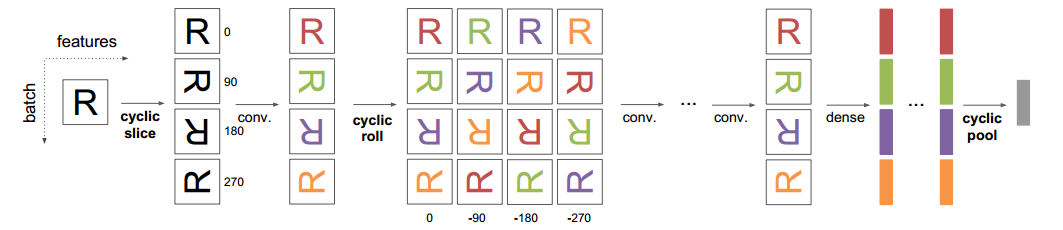
\includegraphics[width=\textwidth]{resources/2_exploting_symmetry.png}
    \caption{The design proposed by Dieleman \textit{et al.} \cite{cyclic_symmetry} to exploiting cyclic symmetry in convolutional neural networks. }
    \label{fig:cyclic_symmetry}
\end{figure}

To exploit cyclic symmetry in convolutional neural networks, Dieleman \textit{et al.} \cite{cyclic_symmetry} introduces four operations that could be used as layers in the design neural network models, enabling partially equivariant to rotations. Cyclic slicing operation produces different rotated versions of input data and stack them into a single batch of training data, while cyclic pooling operation combines different predictions from different rotated copies of input data, merging the batch data created by cyclic slicing operation into a unified one. These two operations focus on converting the space between the input and output while maintaining the equivariance, for example slicing converting the input space to feature space. Cyclic rolling is specially designed to preserved the equivariance in the feature space, which creates the dictionary of all of different rotated versions of extracted features. These features are stacked by cyclic stacking in a mathematics way to preserve the equivariant features. Figure \ref{fig:cyclic_symmetry} visualizes their pipelines to incorporate this property to the network design. Despite the generalization for 90-degree rotation, the extracted features are also partially shown the equivariance to other degrees, which indicates the effectiveness of this design. 

\begin{figure}[thb]
    \centering
    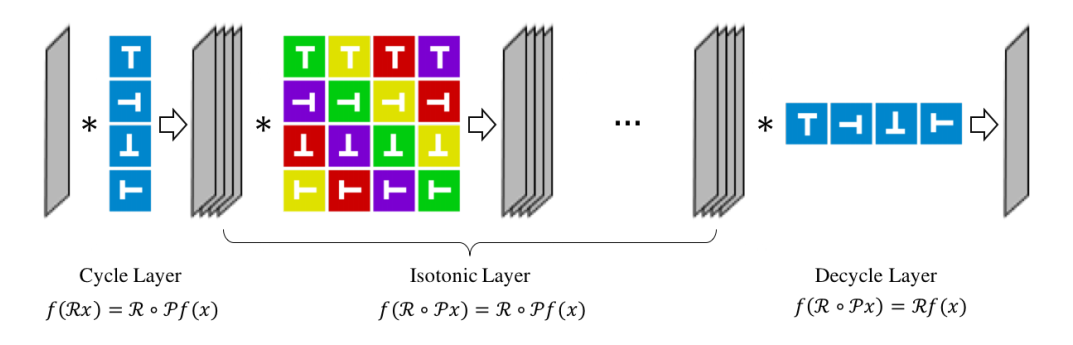
\includegraphics[width=\textwidth]{resources/2_dren.png}
    \caption{The enhancements in the implementation proposed by Li et al. \cite{dren}. Instead of rotating on the feature maps as \cite{cyclic_symmetry}, this method rotates the filters of neural network, saving a lot of memory consumption in the training and inference time.}
    \label{fig:dren}
\end{figure}

Rotating features in the feature space does not require to design any new special layers apart from the current design of vanilla convolutional neural networks. However it consumes a lot of memory because storage of different rotated features. Seeing this pain point, Li et al. \cite{dren} proposed a new approach to implement this idea. Instead of rotating features, they rotate the weights of neural network and use equivalent transformations to create final prediction. All of the proposed layers share the merit with the design from \cite{cyclic_symmetry}. The filters are much smaller than the features, which decrease a huge amount of memory consumption. Figure \ref{fig:dren} visualizes their enhancements in the implementation ideas which are applied on the filters of the neural network, instead of on the feature maps as in figure \ref{fig:cyclic_symmetry}.

Two previous approaches aim to cooperate 90-degree rotation equivariance to the neural network. Marcos \textit{et al.} proposed RotEqNet \cite{DBLP:journals/corr/GonzalezVKT16} to increase the number of rotation degrees that network could produce the equivariant features. Despite freeing the network from learning different features of set of transformed input data, both of two mentioned methods require to store different rotation of features or filters, which partially increases the model size as well as the runtime memory usage. Instead of storing all of the combination of rotated features, RotEqNet \cite{DBLP:journals/corr/GonzalezVKT16} uses the 2D vector filed, which captures the magnitude and orientation of the maximum value across the feature maps. Figure \ref{fig:vector_field} describes their ideas in more detail. Basing on the group theory, Cohen and Welling create a mathematics framework \cite{gcnn} to generalize the equivariance requirement to set of transformations. This does not limit the network on the type of transformations that could be cooperate to its feature representation. For example, the group \textit{p4m} includes the composition of translations, mirror reflections and rotations by 90 degrees about any center of rotation in the grid \cite{gcnn}. The details of this method are discussed in chapter \ref{chap-method}. 

\begin{figure}[thb]
    \centering
    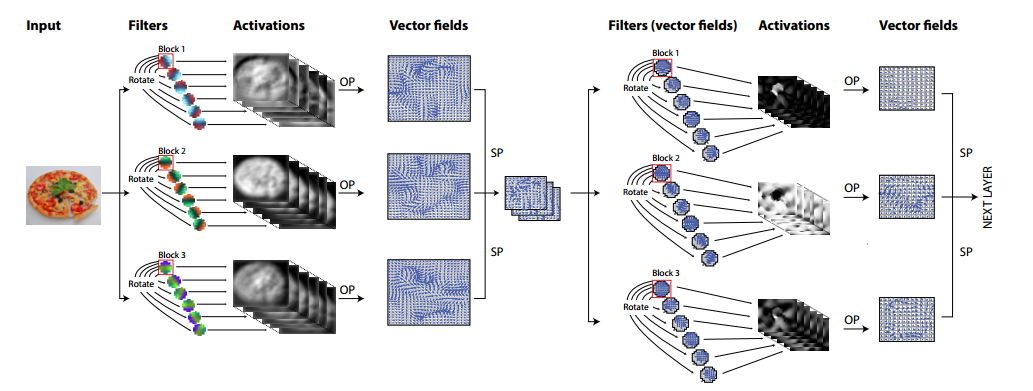
\includegraphics[width=\textwidth]{resources/2_vector_field.png}
    \caption{The RotEqNet proposed by Marcos \textit{et al.} \cite{DBLP:journals/corr/GonzalezVKT16}. This network aims to compact the model in terms of the number of trainable parameters while increasing the amount of number equivariant rotation degrees.}
    \label{fig:vector_field}
\end{figure}

\begin{ChapAbstract}
In this chapter, we give an overview of some works on image classification, object detection, semantic segmentation and instance segmentation. The approach in abnormal findings and anatomy landmark detection in endoscopic image analysis together with nuclear segmentation are discussed in more details. Moreover, we also present the equivariance definition as well as its application in deep neural networks.
\end{ChapAbstract}
%\chapter{Endoscopic Image Classification with Symptom-Localization \&  Data Augmentation}
%Proposed methods for abnormality finding and landmark detection for endoscopic images
\label{chap-method-endoscopy}
\begin{ChapAbstract}
In this chapter, we present our proposed method for abnormal finding and landmark detection in endoscopic images. Particularly, our proposed methods are used to take part in two challenges, including the Medico: The 2018 Multimedia for Medicine Task (Medico 2018) and The Biomedia ACM MM Grand Challenge 2019 (Biomedia 2019). Details about our approaches and improvements between two challenges are also reported. In sum, We utilize different  deep convolution neural network architectures together with several training techniques to improve the overall performance.
\end{ChapAbstract}

\section{Overview of proposed methods}
To tackle with the image classification problem, we consider using a stacked model consisting of two deep networks, a Residual Neural Network (ResNet) followed by a Faster Region-based Convolutional Neural Network (FasterR-CNN). We carefully analyze the results after each intermediate steps to understand about the properties of each module. As our observation, the image classification already proposed significant results in term of the accuracy on our validation set. However, it fails to classify images that abnormal symptoms of diseases or instruments appeared as  small objects on diversity backgrounds. It happens because of the ResNet mostly focuses on deep global features of image, when we just feed all of them into the network. Therefore, this is the reason of using Faster R-CNN to re-classify the images of some classes that ResNet usually mis-classifies. 

Nevertheless, inference time must be taken into account, while the Faster R-CNN needs longer time to process than that of ResNet. Therefore, instead of feeding all images through the ResNet module, we should have a strategy that reduce the number of images need to go through the Faster R-CNN module. We propose several configurations as our official submissions, as presented in Section \ref{5runs_config}.

Besides, due to the diversity of endoscopic images, various kind of abnormalities can appear in one image, that image can be classified into multiple classes simultaneously. Regarding to this  Multi-class classification problem, the task organizers of the Medico 2018 propose a priority list which forces every systems of participants should return only one class which has the most important level compare to others. In Medico 2018, we tried to force our model by re-organize the training set together with adding extra training samples in order to help our model can learn that priority list. However, we found out that it is also possible to propose a multi-task classification architecture that can predict multiple classes at the same time, which can reduce the confusing level of the image classifier model in these difficult cases. Further information about this architecture is presented in Section \ref{sec:multi_task}.
 
In the development dataset, there is an unbalance between classes and false labeling which are commonly occurred in medical dataset. Unbalancing between classes can make deep models bias to some classes than others, which reduce the overall accuracy. Moreover, one of the goals of these challenge is using as less as training data as possible, therefore, using extra data from other dataset is not possible in this case. Nevertheless, in order to build the object detection model as we mentioned before, extra information about the location of symptoms must be given, i.e bounding boxes can be used to localize these locations. Regarding to mentioned problems, in this work, besides annotating symptoms of diseases which is described in Section \ref{sec:symptoms_local}, we also provide some augmentation mechanism on the given training dataset in order to provide a better version for the training step of both Faster R-CNN module and ResNet module. See Section \ref{sec:augment} a complete description of our work related to our data augmentation strategy.  

\section{From Classification to Symptoms Region Localization}
\label{sec:symptoms_local}
Obviously, to enhance the performance of our system, an object detection module can be really useful to detect small abnormal symptoms and diseases, such as \textit{polyps, instruments, dyed-lifted-polyps} and \textit{dyed-resection-margins}. Besides, in some cases that multi-symptoms appear in the same image, identify all of them is necessary to draw the final conclusion. Nevertheless, system that can not only predict the abnormalities but also propose the corresponding positions of that is more reliable and more convenient for endoscopists. Estimating the sizes of these abnormalities can  become really efficient for future systems. 

In order to train an object detection model, besides an images dataset, we also need the corresponding bounding boxes for each abnormality and passed them to the model as input during the training phase. 

Due to the limitation of the given training dataset, there is no extra information about positions of abnormalities inside image  given. Therefore, in our first step, we decided to annotate all the abnormal symptoms in every images of the following classes: \textit{dyed-resection-margins, dyed-lifted-polyps, instruments} and \textit{polyps} with the help of the LabelImg \footnote{\url{https://github.com/tzutalin/labelImg}} annotation tool. Examples of our proposed bounding box can be seen in Figure \ref{fig:symptoms_localization}.

\begin{figure}[thb]
\begin{center}
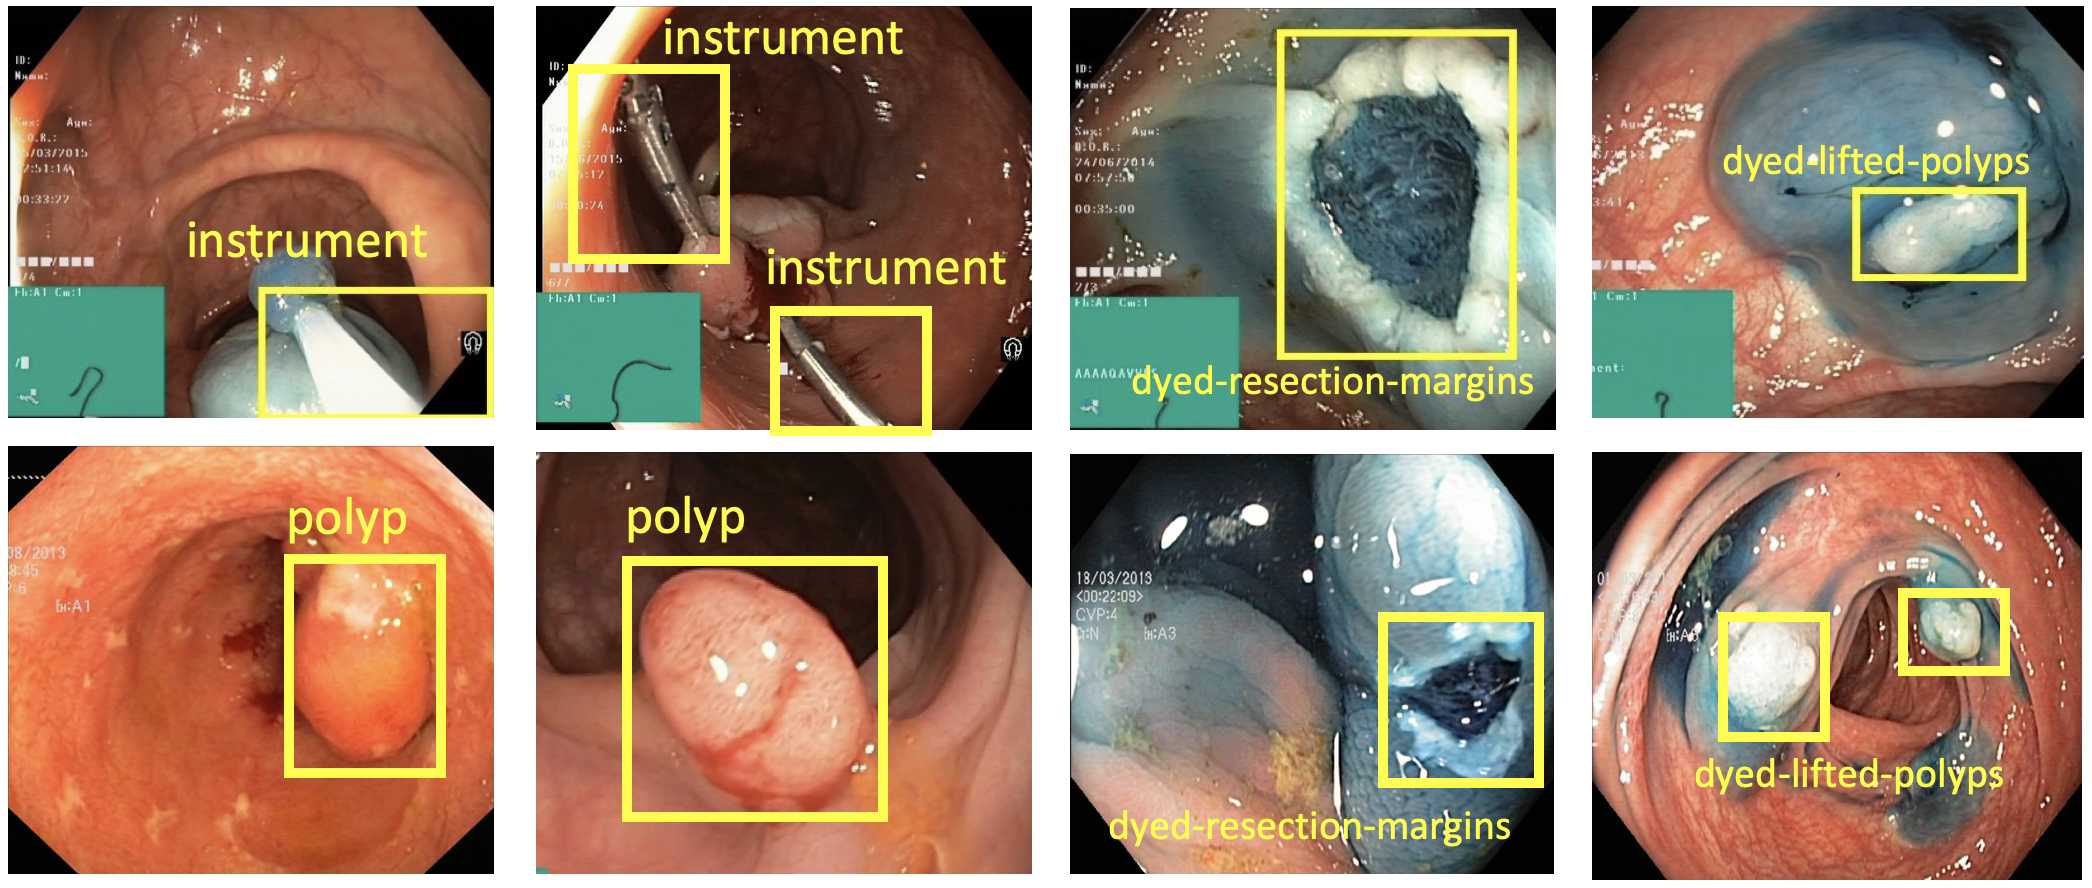
\includegraphics[width=\textwidth]{endoscopy_resources/symptoms_region_localization.png}
\end{center}
   \caption{Our proposed symptoms region localization, annotated images with corresponding bounding boxes and classes name.}
\label{fig:symptoms_localization}
\end{figure}

Totally, with 5241 images belong to the following classes: \textit{polyp, dyed-lifted-polyp, dyed-resection-margins} and \textit{instruments} category are annotated with 5715 bounding boxes from the Kvasir dataset \cite{Pogorelov:2017:KMI:3083187.3083212} and Medico 2018 development dataset. The number of bounding boxes for each class is reported in Table \ref{tab:count_bbox}. Although, the number of training samples we annotated is much larger than the number of actual training samples we used in training phase, it is still useful for future works. 

\begin{table}[tbh]
\caption{Number of annotated bounding boxes from each class.}
\centering
\begin{tabular}{|l|c|}
\hline
\multicolumn{1}{|c|}{\textbf{Class}} & \textbf{Number of bounding boxes} \\ \hline
\textit{dyed-lifted-polyp}                    & 1513                              \\ \hline
\textit{dyed-resection-margin}                & 1509                              \\ \hline
\textit{polyp}                                & 2657                              \\ \hline
\textit{instruments}                          & 36                                \\ \hline
\multicolumn{1}{|c|}{Total}          & 5715                              \\ \hline
\end{tabular}
\label{tab:count_bbox}
\end{table}

\section{Addition Labeling for \textit{Instruments} versus Other Classes}
As our viewpoint, the \textit{instruments} and \textit{polyps} are classes that are likely to appear together with other classes. We decided to annotated and mark every image in the development dataset which contains \textit{instruments}/\textit{polyps} or not. These addition labels are useful for us to train the Multi-task classification network which is further described in Section \ref{sec:multi_task}.

\section{Instruments Dataset Augmentation}
\label{sec:augment}
\textit{Instruments} - the second highest priority class has only 36 images with the limitation of background context in the Development set of Media Eval 2018. 

In order to maintain the balancing between all of these classes and also improve the diversity of the \textit{instruments} images, we aim to augment the given dataset by generate more images for the \textit{instruments} based on the current given development set by placing the instruments on the foreground of other diseases backgrounds.

Among the 36 \textit{instruments} images, we carefully select 24 of them and crop the instruments along their edges. Then, we randomly select images from \textit{dyed-lifted-polyps, dyed-resection-margins}, \textit{ulcerative-colitis} classes, and use them as the background of the cropped instruments. By applying this method, we are able to generate more than 800 images for the \textit{instruments} class. The overview of this process is illustrated in Figure \ref{fig:instruments_augment}.

\begin{figure}[thb]
\begin{center}
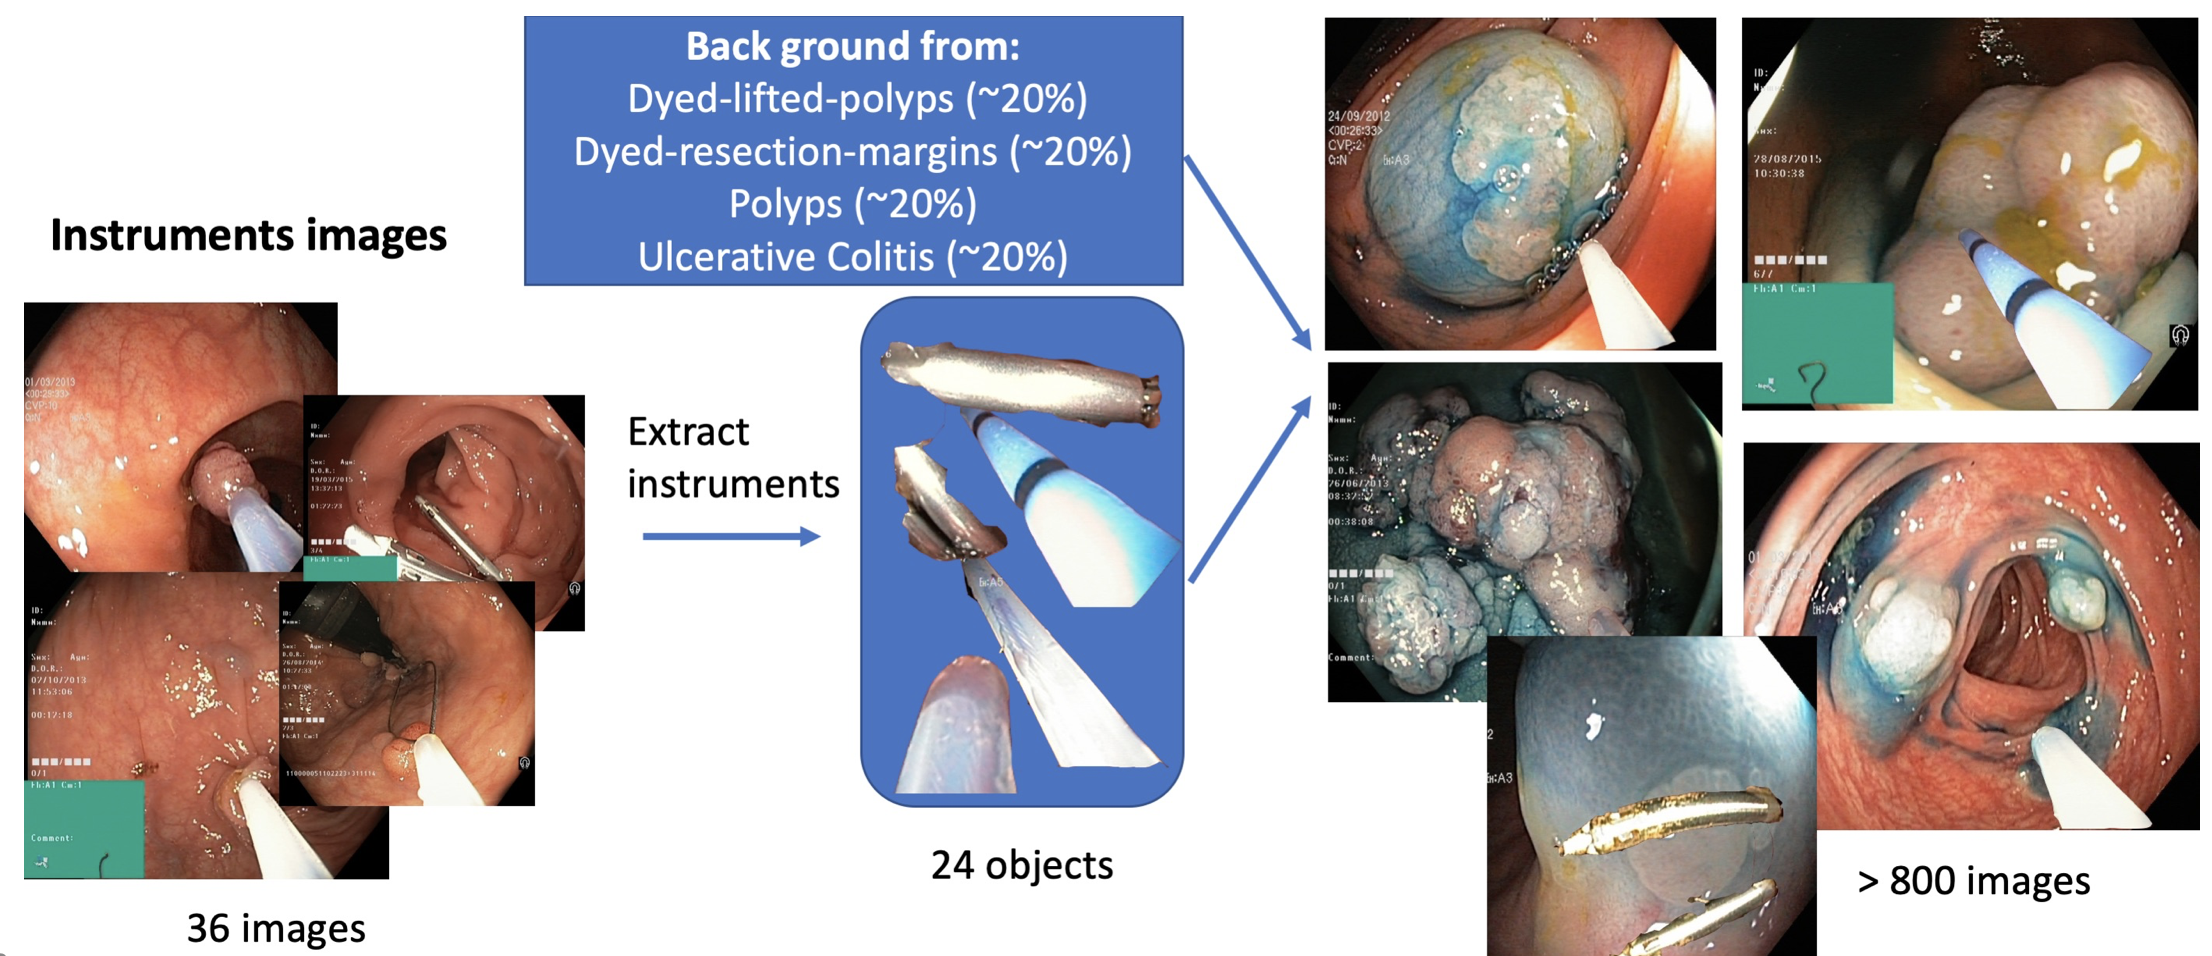
\includegraphics[width=\textwidth]{endoscopy_resources/instruments_augmentation.png}
\end{center}
   \caption{Overview of the \textit{Instruments} dataset augmentation process.}
\label{fig:instruments_augment}
\end{figure}

\begin{figure}[thb]
\begin{center}
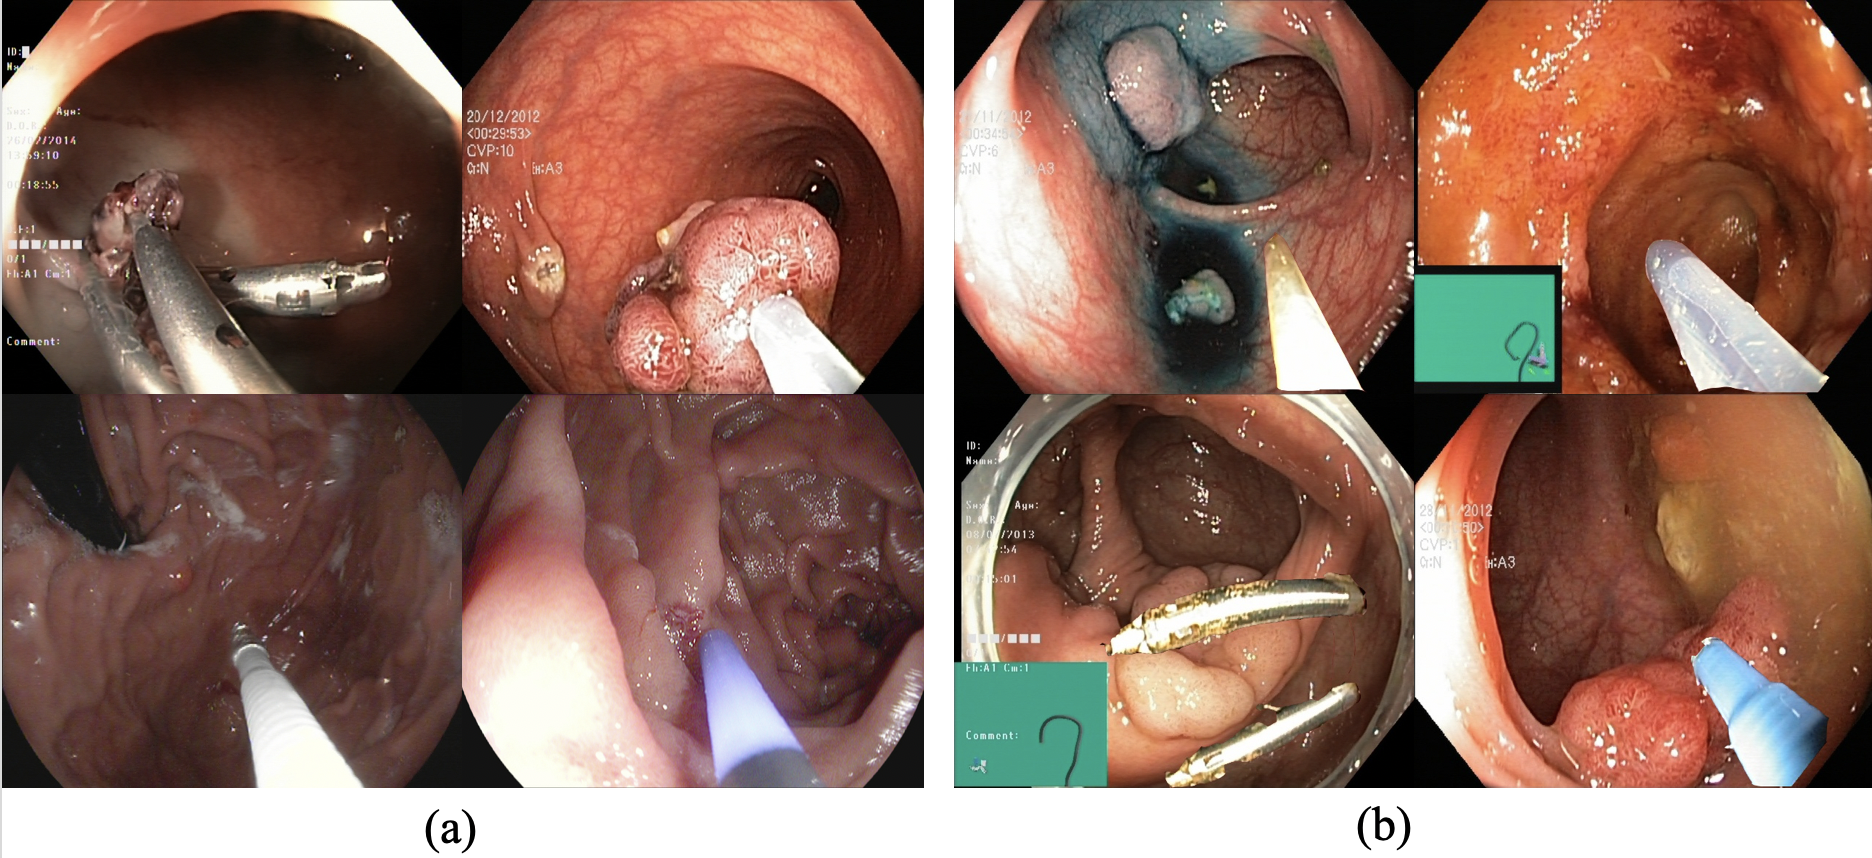
\includegraphics[width=\textwidth]{endoscopy_resources/instr_augment_compare.png}
\end{center}
   \caption{\textit{Instruments} dataset augmentation result. (a) original \textit{instruments} images in development dataset. (b) augmented \textit{instruments} images generated by our method}
\label{fig:instruments_augment_compare}
\end{figure}

\begin{figure}[thb]
\begin{center}
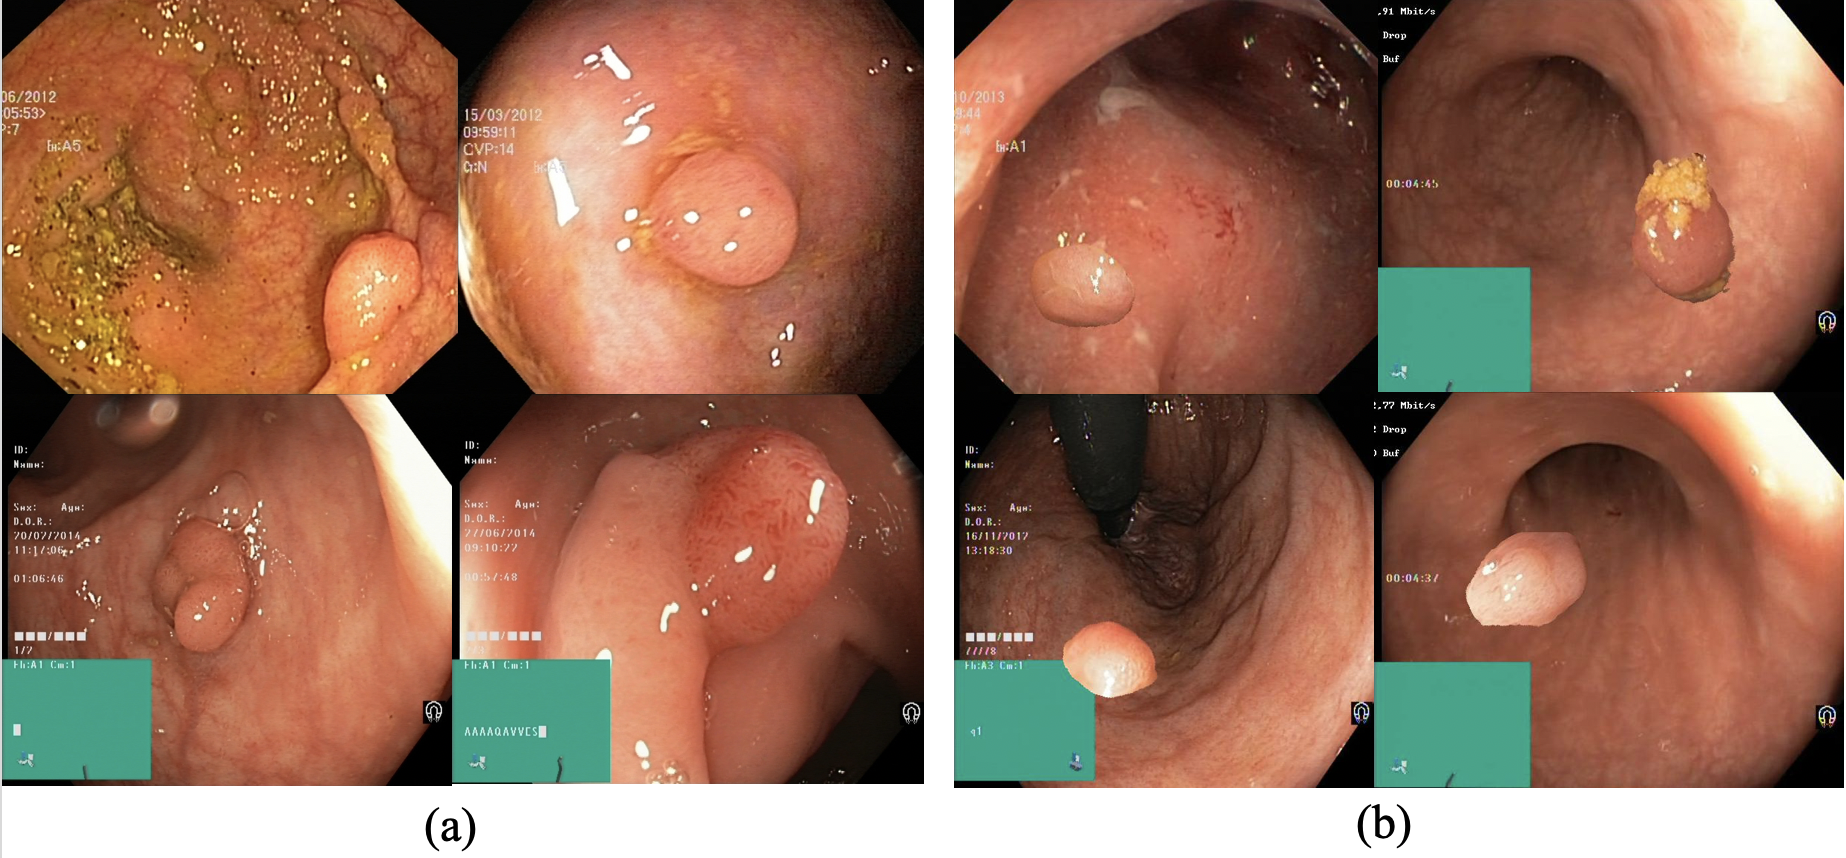
\includegraphics[width=\textwidth]{endoscopy_resources/polyp_augment_compare.png}
\end{center}
   \caption{\textit{Polyps} dataset augmentation result. (a) original \textit{polyps} images in development dataset. (b) augmented \textit{polyps} images generated by our method}
\label{fig:polyps_augment_compare}
\end{figure}

Figure \ref{fig:instruments_augment_compare} illustrates samples belong to the \textit{instruments} class, including  the  original samples and augmented samples. Similarly, Figure \ref{fig:polyps_augment_compare} demonstrates the augmentation result on the \textit{polyps} class. As our observation, there is not significant visual differences between samples from two groups. 

The augmented dataset can be used for both sub-task. By adding more positive examples to the training phase of the classification model, the performance of this model can be more robust. On the other hand, we  can easily get the position of the foreground object on generated images, which can be utilized to augment the training dataset of the objects detection module (Faster R-CNN). 

\section{Proposed system}
% 1) overview co re nhanh cac kieu
% 2) Mootj trong nhung cach endcode mot tam hinh, thay vi dung cai co san, dung 1 cai specialize , duoc dung  cho ca 2 task train end to end
% 3) Train Faster R-CNN 
\subsection{Overview}
Our approaches focus on utilizing the advantages of both object detection, such as Faster R-CNN and image classification, such as ResNet 101. However, due to the criterion of the endoscopy diagnosis system, the inference time of both modules must be taken into account. Noticeably, this number in Faster R-CNN is much larger than ResNet 101. By carefully observe the intermediate results of each module, we proposed several conditional strategies that limit the number of images feeding into the object detection module based on the  prediction  of image classification  module. In order to figure out the most balancing configuration for our method, multiple scenarios have been proposed and evaluate. Details about these configuration are presented in Section \ref{fig:5runs}.

\subsection{Fine-tuning Deep Neural Network on Endoscopic images}
Besides high computational cost, one of the main drawback of deep learning architecture is that it requires a large amount of training data. Moreover, labeled medical data
for supervised learning is limited and manual labelling of medical images is a difficult task. Therefore, it requires a lot of effort and time to train the network, which would depend on the size of training data used. However, there is a possible solution to deal with these limitations is
using transfer learning, where a pre-trained network on a large dataset (such as ImageNet \cite{ImageNet}) is used. 

In our approach, both Residual Network with 101 layers and Faster R-CNN \cite{chen17implementation} are both share a same features encoder. Therefore, it is necessary to propose a features encoder that is specialized on endoscopic images. This is the reason that we fine-tuned our deep neural network models (pre-trained on ImageNet) by using our modified development dataset. After training the whole neural network and then we freeze several first layers in its architecture and fine-tune the remains with small learning-rate. We also tried to train the network from scratch and all of our experiments point out that in term of using convolution neural network for medical images, knowledge transferring from natural images to medical images is possible, even though there is a large difference between the source and the target databases. 


This idea is also mentioned in \cite{trainingorfinetune}, it is especially useful in the case of small dataset of images provided. Fine-tuning on the ImageNet pre-trained model significantly improves the efficient of deep learning model on medical domains.

\section{Configuration of Conditional Scenarios}
\label{5runs_config}

\begin{figure}[tb!]
\begin{center}
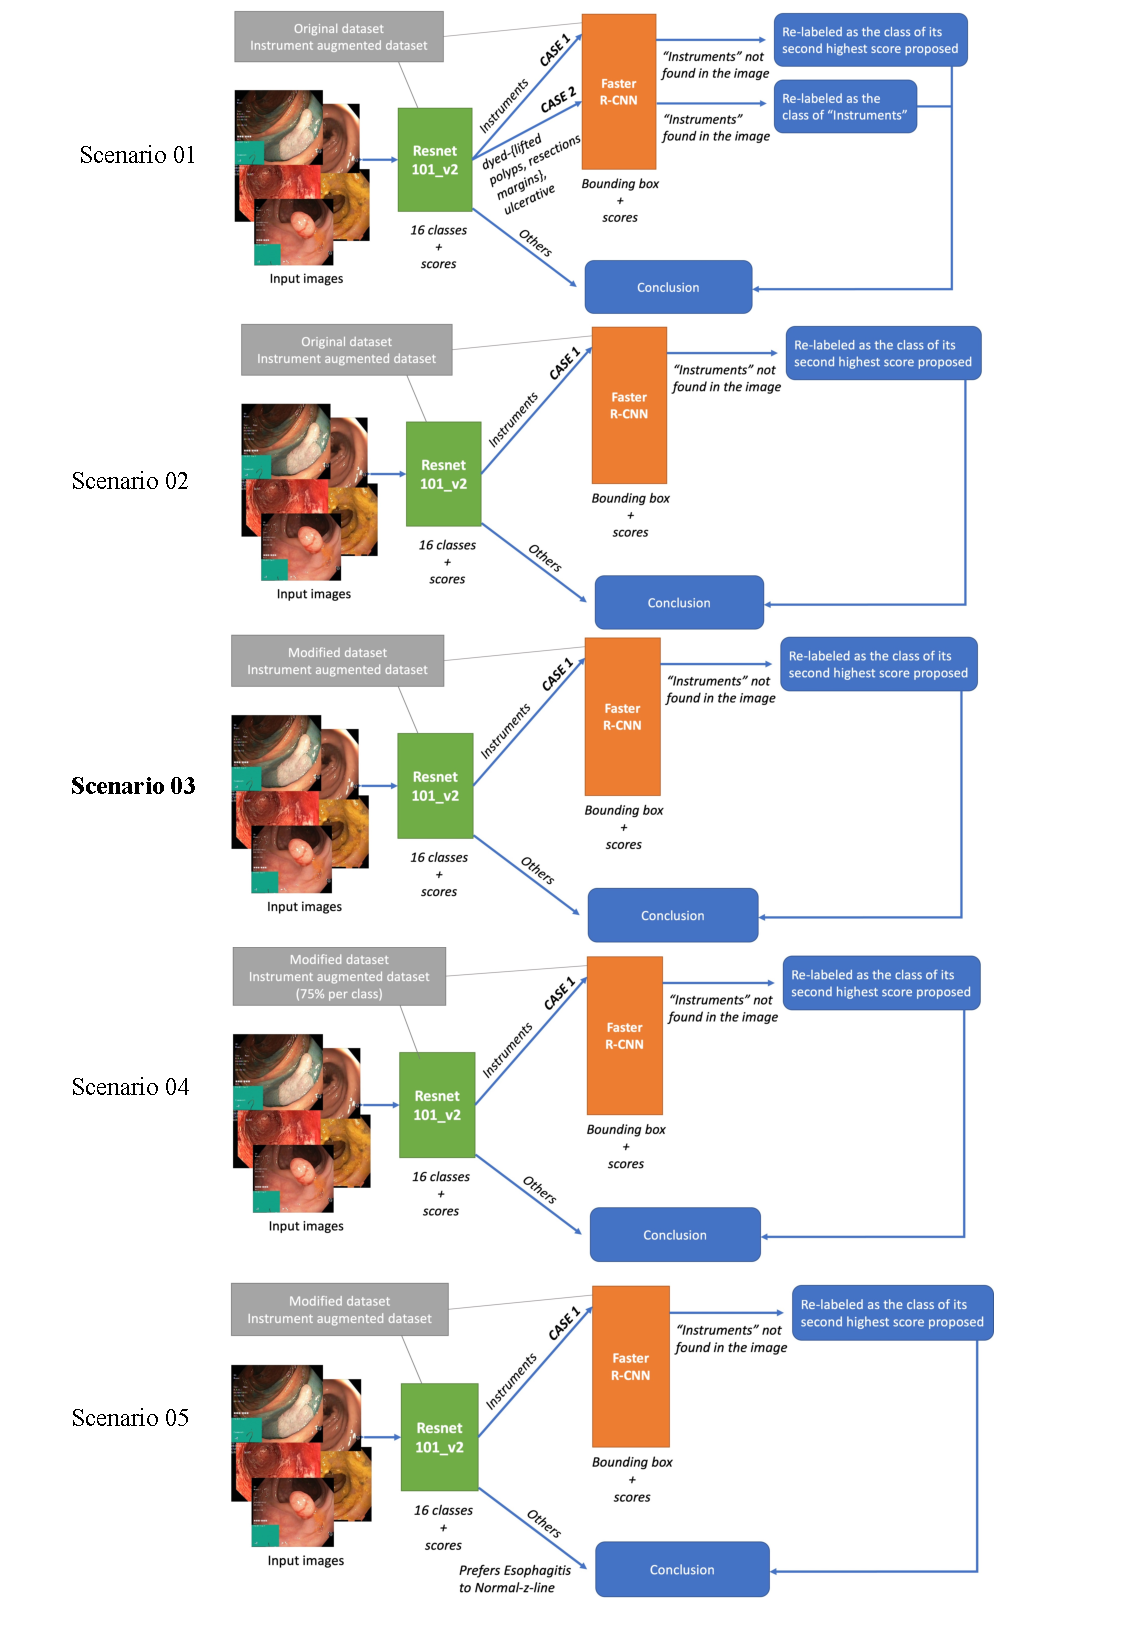
\includegraphics[scale=0.75]{endoscopy_resources/5runs.pdf}
\end{center}
   \caption{Overall process configuration for 5 scenarios.}
\label{fig:5runs}
\end{figure}


As mentioned before, there is a trade-off between the inference time and the accuracy. 
% In Medico 2018, we tried several configurations for our submissions (called \textit{Run}). Totally, we submitted 5 \textit{runs} to organizers. 
The following section describes the pipeline for each of our \textit{runs}. Figure \ref{fig:5runs} illustrates in image. Note that, the \textit{Scenario 03} has performance the best in term of the accuracy while \textit{Scenario 02} has the best inference time. Details and comments about the official evaluate result for each run are further discussed in Section \ref{sec:medico2018_results}.

\subsection{First scenario: \textit{instruments, polyps} double-checked}
Residual network with 101 layers model are fine-tuned on the original development set provided by the task organizers along with our instruments increased dataset. After passed through ResNet101, output images classified as special classes become the input of Faster R-CNN network, which is trained for detecting instruments in images.

\begin{itemize}
    \item First case: Images predicted as \textit{instruments} by Resnet101 are double-checked. In case instruments are not detected by Faster R-CNN in those images, they are re-labeled as the class of their second highest score proposed by Resnet101. %classifier.  
    \item Second case: Images predicted as \textit{dyed-lifted-polyps, dyed-resection-margins, ulcerative colitis} by ResNet101 are fed forward through Faster R-CNN network to detect \textit{instruments}. They are classified as \textit{instruments} if detected or keep the original prediction otherwise.
\end{itemize}

\subsection{Second scenario: \textit{instruments} double-checked}
Feeding forward a large number of images in the three classes through Faster R-CNN causes a bottle-neck of inference time, as Faster R-CNN has high time complexity.
% , around 0.8 second for each image. 
Therefore, in this second , we limited the images passed through Faster R-CNN by only performing the first case of the first scenario.

\subsection{Third scenario: \textit{instruments} double-checked and data augmentation}
The configuration of the third scenario is as same as the second scenario. Instead of using the original training set mentioned in the first scenario, we train our model on the re-labeled development set combined with the augmented instrument set.

\subsection{Forth scenario: 75\% of training set}
In this scenario, we reduce the number of images used for training by selecting randomly 75\% images of each class in the same training set as the third scenario. Other processing steps are also configured in the same way.

\subsection{Fifth scenario: \textit{esophagitis} priority}
Throughout our experiments,
% we realize that the two classes 
\textit{normal-z-line} and \textit{esophagitis} are the top most confusing classes not only for Resnet101 but also for human to distinguish them. In the priority list, \textit{esophagitis} has a higher rank than \textit{normal-z-line's}. Thus, after several times evaluating our model on the development dataset, we propose a condition for these two classes when they are predicted by ResNet101. As ResNet101 provides a probability distribution over the 16 classes for each image, whenever the 
\textit{normal-z-line} appears to be the highest class, we add a small bias $0.3$ to the probability of the \textit{esophagitis}. Hence, the model is more likely to emit the \textit{esophagitis} class. This intuitively means that our model prefers \textit{esophagitis} to \textit{normal-z-line} when it is confused between these classes.

\section{Solving Multi-class Problem with Multi-tasks Classifier}
\label{sec:multi_task}
After Medico 2018, another improvement of our work is to reduce the confusion level of the deep neural network model in cases that various type of abnormalities appeared in a same image. Instead of using only one classifier and forcing the deep neural network model to follow the priority list in these cases by feeding a number  of positive and negative samples, we narrow down this job to multiple classifiers. For instance, given an image that both \textit{esophagitis} and \textit{instruments} appear simultaneously, the job to determine whether or not \textit{instruments} appear inside the image is then left for a 2-classes classifier. This classifier can output the probability that the  given image contains \textit{instruments}. Meanwhile, the  second classifier works independently, which can output the probability for other classes, except \textit{instruments}.

\subsubsection*{Architecture}
In order to reduce the inference time, we decide to share the weights of backbone ResNet 101 for both classifier. The overview of this module can be seen in Figure \ref{fig:multitask_overview}. In general, the proposed multi-task classification model consists of a ResNet 101 architecture except the last fully connected layer, working as a features extractor module that can output a 2048 dimensions vector for  each input image. There are two fully connected branches on top of the output of that features extractor in order to get the prediction of \textit{instruments} class and other 15 \textit{classes}. The number of classifiers is extendable in the future.

\subsubsection*{Loss function}
Two classifiers are trained simultaneously with the overall loss function is a weighted sum of each of their loss, given as follow 
\begin{equation}
       \mathcal{L}(p_i, p_o,p_i^{*},p_o^{*}) = \lambda\sum_{i} \mathcal{L}_{instruments}(p_i, p_i^{*}) + (1-\lambda)\sum_{i}\mathcal{L}_{others}(p_o, p_o^{*})
\end{equation}
where $(p_i,p_i^{*})$ and $(p_o,p_o^{*})$ denote the prediction and the ground-truth of \textit{instruments} class and other classes, respectively. $\mathcal{L}$ is Cross Entropy Loss function. $\lambda$ is a combination weight.

\begin{figure}[H]

\begin{center}
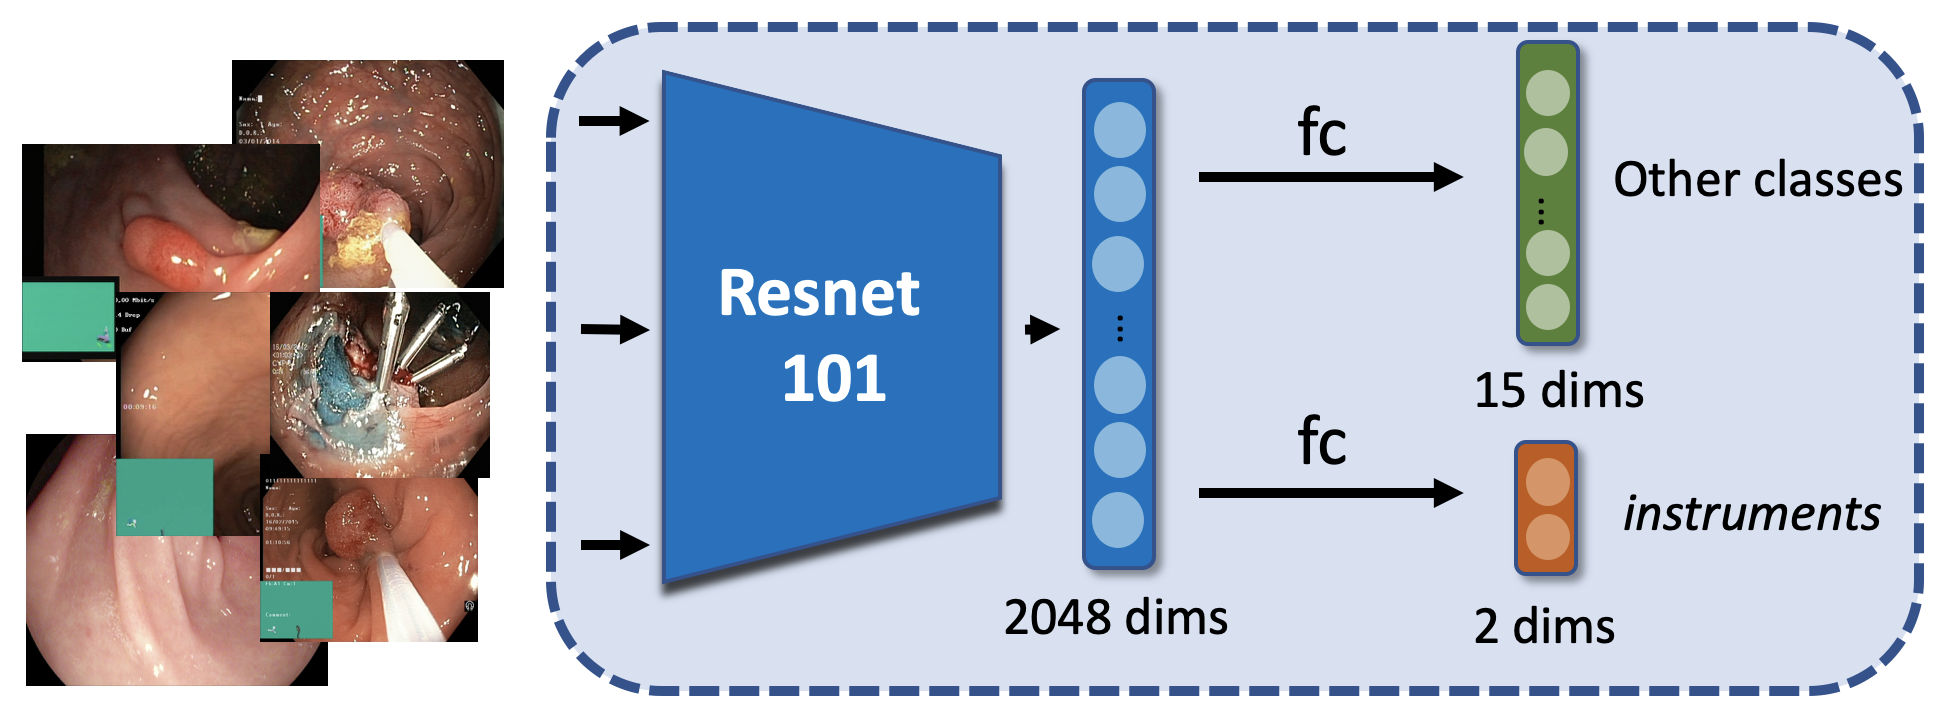
\includegraphics[width=0.8\textwidth]{endoscopy_resources/multi-task.png}
\end{center}
   \caption{Overview of the Multi-class classifier network.}
\label{fig:multitask_overview}
\end{figure}

\subsubsection*{Final prediction}
Since, there are two output vectors from the model, the final prediction can be determined by 

\begin{equation}
    y_{f} = \begin{cases}argmax(p_{o}) & p_{i} < 0.5\\y_{instruments} & p_{i} \geq 0.5\end{cases}
\end{equation}

where $y_{f}$ stands for the final prediction of input image, $p_{o}$ is a 15 dimensions vector indicates the probability that image is likely to belong to. $p_{i}$ is the probability that \textit{instruments} appear inside the image and $y_{instruments}$ is the corresponding label of \textit{instruments} class.

\section{Configuration of Submissions for The Biomedia ACM MM Grand Challenge 2019}
\label{5runs_config}
For the Biomedia ACM MM Grand Challenge 2019 challenge, we continue to tackle existing problems that we did not solve efficiently in Medico 2018, which are the confusing between \textit{normal-z-line} and \textit{esophagitis}; Multi-class problem with \textit{instruments} classes. Besides increasing the size of training data with our augmentation strategy, there are two major improvements in this challenge.
\begin{itemize}
    \item (1) With the Multi-class problem, \textbf{we applied the Multi-tasks Classifier} which is introduced in \ref{sec:multi_task}.
    \item (2) With the \textit{normal-z-line} and \textit{esophagitis}, with a help of a medical expert, we re-annotate the labels of the original dataset and train our models on the modified version of the dataset.
\end{itemize}

In order to evaluate our new improvements to the overall performance of the system, we applied several configurations as given in Table \ref{tab:biomedia_config}.

\begin{table}[h]
\centering
\caption{Experimental configurations for The Biomedia ACM MM Grand Challenge 2019. Character $\bullet$ denotes the corresponding improvement is applied.}
\begin{tabular}{|c|c|c|}
\hline
\multicolumn{1}{|l|}{\textbf{Runs ID}} & \multicolumn{1}{l|}{\textbf{(1)}} & \multicolumn{1}{l|}{\textbf{(2)}} \\ \hline
\textbf{01}                            &                          &                          \\ \hline
\textbf{02}                            & $\bullet$                        &                          \\ \hline
\textbf{03}                            &                          & $\bullet$                        \\ \hline
\textbf{04}                            & $\bullet$                        & $\bullet$                        \\ \hline
\end{tabular}
\label{tab:biomedia_config}
\end{table}

\begin{ChapAbstract}
In this chapter, we discuss the main challenges in applying deep neural network to solve image classification and object detection task on endoscopic image dataset. Especially, we also describe our approaches to overcome mentioned challenges, which can be extend to solve these problems in similar situations.
\end{ChapAbstract}

%\chapter{Enhanced Rotation-Equivariant U-Net for Nuclear Segmentation}
\label{chap-method}
\begin{ChapAbstract}
In this chapter, we present our proposed method for nuclear segmentation in H\&E stained histopathology images. Specifically, we consider enforcing rotation equivariance in the network, the placement of residual blocks, and applying novel data augmentation designed specifically for histopathology images, and show the relative improvement and merit of each. Incorporating all of these enhancements in the design and training of a U-Net yields significantly improved segmentation results while still maintaining a speed of inference that is sufficient for realworld applications, in particular, analyzing whole-slide images (WSIs).  
\end{ChapAbstract}

\section{Overview of proposed methods}
The recent surge in interest in deep learning coupled with increasing availability of large-scale histopatholical image data sets, such as The Cancer Genome Atlas \cite{tcga}, has resulted in significant advances in computational histological analysis \cite{he_dataset_kumar, unet}. A crucial step in such analysis pipelines is accurate and efficient segmentation of cell nuclei \cite{review_seg_overall}. With the aid of large-scale training data, deep-learningbased methods for automatically segmenting nuclei have surpassed traditional approaches, such as watershed \cite{watershed}
and thresholding \cite{Otsu} algorithms, though, despite these improvements, this step remains challenging and continues to be an active area of research \cite{review_seg_overall}. Changes in nuclear morphology are well-studied indicators of diseases, such as cancer, which motivates the continued development of effective methods of automated segmentation.

Initial approaches using deep learning operated by scanning the image patch-by-patch and generating a label (e.g., nucleus or non-nucleus) for each pixel centered in each patch \cite{he_dataset_kumar}. Subsequent morphological processing could be applied to help smooth and refine the generated label masks and ensure that the segmented regions are contiguous. More recently, the U-Net architecture was proposed \cite{unet}, which operates on the entire image and jointly infers the label at each pixel simultaneously, leading to more spatially coherent segmentation. U-Nets have been shown to achieve improved accuracy on several bioimage segmentation tasks, even when the data set is relatively small \cite{unet}.

In this work, we bring together several recent developments in bioimage analysis to enhance the current methodology for deep-learning-based nuclear segmentation and, through a thorough ablation study, show the relative improvement and merit of each. We show that combining these enhancements together can achieve significantly improved scores for several important metrics at a speed that
is sufficient for real-world applications, such as analyzing
whole-slide images (WSIs). In more detail, enforcing rotation equivariance in the network, the placement of residual blocks, and applying novel data augmentation designed
specifically for histopathology images are proven to overcome challenges not only in nuclear segmentation but also other related domains such as astronomy data through the relative improvements. Section \ref{sec:main_challenges} discusses the main challenges not only in the nuclear segmentation field but also other related domains as well as overview of our enhancements to overcome these problems. The merit of each enhancement will be described in more detail in section \ref{sec:proposed_method}. 

\section{Main indicated challenges}
\label{sec:main_challenges}
\subsection{Equivariance to rotation \& translation group}

As proven in \cite{gcnn}, the convolutional neural networks are effective because of weight sharing mechanism, which activates the translation symmetry in most perception task. It means that the feature of shifted version of image feeded to the network is same as the shifted feature of the original images plugged to the same network. However, when it comes to other transformation such as rotation, reflection, etc. the designed architecture fail to maintain such equivariance properties. This limits the generalization of the results produced from these kind of architectures, especially in many filed such as microscopy image segmentation, astronomy analysis, ... To overcome this challenge, especially in nuclear segmentation problem, the first enhancement to the U-Net we consider is to encode equivariance to groups, specifically rotation and translation, following the work of group-equivariant CNNs (GCNNs) \cite{gcnn}, thereby obviating the need to learn such equivariance through extensive and time-consuming data augmentation. This enhancement helps the learned network to better generalize to such variation in unseen data. G-CNNs have recently been shown to demonstrate top performance on segmenting regions of interest in histology images \cite{DBLP:journals/corr/abs-1806-03962} and biological structures in other types of bioimages \cite{DBLP:journals/corr/abs-1804-03393}, but have not yet been applied to the task of nuclear segmentation.

\subsection{Limited receptive field for boundary classification}

\begin{figure}[thb]
    \centering
    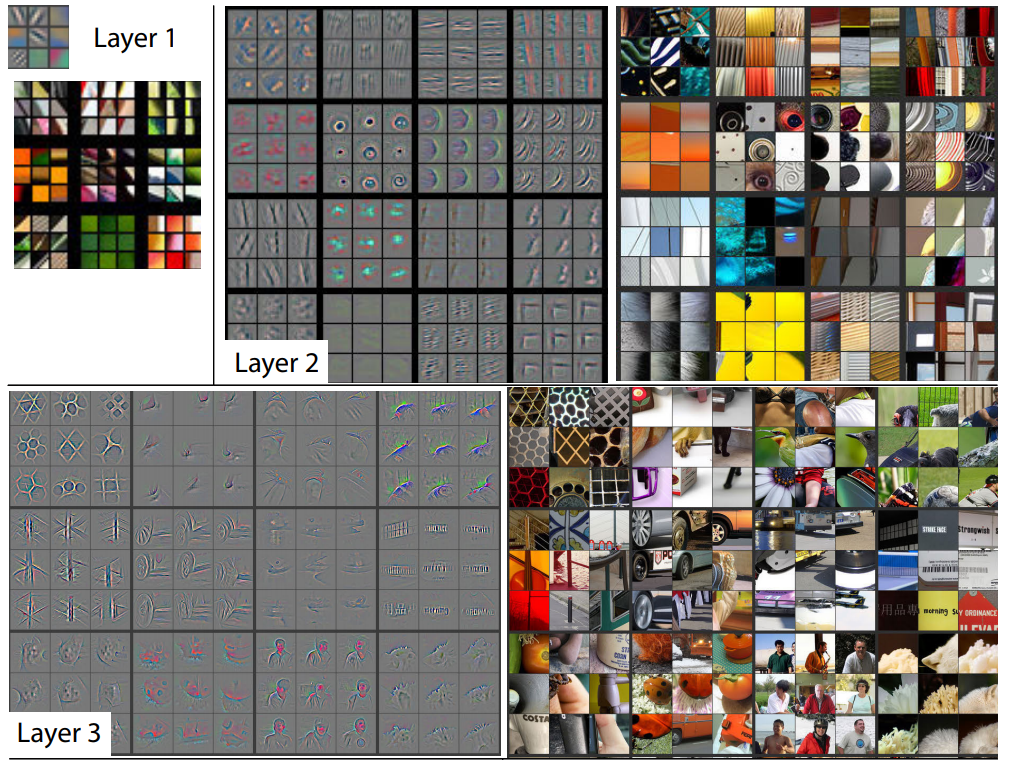
\includegraphics[width=\textwidth]{resources/5_feautures.png}
    \caption{Each layers of networks \cite{ZFNet} are responsible for detecting a type of features (including low-level and high-level one).}
    \label{fig:low_high_features}
\end{figure}

As visualized in figure \ref{fig:low_high_features} from \cite{ZFNet}, the earlier layers of convolutional neural networks are responsible for detecting low-level features such as contour, edge, while the deeper layers detect high-level features like eyes, noses, etc. As this results, the low-level branches of U-Net, which have limited receptive field, focus on analyzing the contours or edges existing in the data. This phenomenon affects a lot on problems require segmenting accurately on the boundary, for example in nuclear segmentation. In this type of problem, to segment correctly the boundary, the network needs to expand its receptive field of these low-level layers to have more information to decide whether the current pixel belongs to boundary class. Therefore, we decide to enhance the long-skip connections in the U-Net from the downsampling to upsamling arms of the “U” with residual blocks, an insight that has shown improved performance for other applications \cite{DeepLabv1}. The motivating hypothesis of this modification is that providing richer low-level features from the downsampling arm, learned through the residual blocks, to the upsampling arm will aid in producing detailed boundaries, especially between touching nuclei. This enhancement is not limited to nuclear segmentation problems but all tasks requiring the accurate boundary segmentation. 

\subsection{Data shortage}

Lastly, we propose a novel means of data augmentation specifically designed for histological images to aid in training. Although the rate of generation of H\&E image data is increasing, fully-labeled training data is still scarce. Therefore, augmentation of training data is still crucial for learning robust models. In addition to standard augmentation techniques of elastic deformations, blurring, and additive noise, we generate synthetic images by slightly translating and deforming the nuclei and filling any empty pixels by inpainting \cite{DBLP:journals/corr/abs-1801-07892}. This method was inspired by recent work in video object segmentation \cite{DBLP:journals/corr/KhorevaBIBS17}, which demonstrated significant improvements in performance. Others works have also proposed means of generating synthetic, realistic histological images \cite{DBLP:journals/corr/abs-1810-00236}, though ours is much simpler to implement. Although this scheme is specialized for nuclear segmentation in H\&E stained histopathology images, it could be applied for other domains such as other microscopy data, video data, etc.

\section{Methods}
\label{sec:proposed_method}
The standard U-Net architecture consists of two arms, one for downsampling the feature maps to a lower-dimensional space and one for upsampling the feature maps back to full resolution.
Each downsampling layer consists of convolution, non-linear activation, pooling, and batch normalization.
Each upsampling layer consists of similar operations except that pooling is replaced by upsampling.
Additionally, residual blocks~\cite{Resnet}, which are used to increase the depth of the network, can be added.
In~\cite{DBLP:journals/corr/HanKK16}, some experiments evaluated the performance of different types of residual blocks.
We inherit from their work the architecture producing the best reported performance. 
Lastly, to help with interpolating the higher-resolution feature maps, features from the downsampling arm are conveyed to the upsampling layers by long-skip connections.
From this baseline architecture, we incorporate two enhancements, namely group-equivariant operations to encode equivariance to rotation and translation, and residual blocks along the long-skip connections.
We describe these enhancements below.

As in other deep-learning-based approaches~\cite{he_dataset_kumar}, we formulate nuclear segmentation as a pixel labeling problem with three potential labels, namely, nuclear interior, nuclear boundary, and background.
The network is designed and trained to produce a probability map for each label.
Creating a label especially for the boundary results in a larger contribution to the objective for boundary pixels and thereby encourages the network to produce a more accurate boundary, which is generally harder to infer by post-processing than pixels away from nuclear boundaries.
Our post-processing method of morphological operations, described below, helps to refine the output of the U-Net by smoothing edges and ensuring contiguous segmentation boundaries.

Input data is first stain-normalized before being fed to the U-Net.
To help train the model, we employ several means of data augmentation, including our proposed histology-specific method, which we describe below. 

\subsection{Encoding group-equivariance}

As noted in~\cite{gcnn}, it is helpful to think of the input image to a neural network as a function $f\colon\mathbb{Z}^{2}\rightarrow \mathbb{R}^{K}$ that maps 2D space to pixel intensities.
The insight of~\cite{gcnn} for CNNs was to generalize equivariance to translation, which is inherent to standard convolution, to other transformations by defining convolution for \emph{groups} in general, of which $\mathbb{Z}^{2}$ with translations is a specific example.
An important group for histology images is the $p4$ group, which consists of translations and rotations about the origin by 90 degrees of elements in $\mathbb{Z}^{2}$.
%and a filter $\psi^{i}\colon\mathbb{Z}^{2}\rightarrow \mathbb{R}^{K}$, both of which operate on the 2D space of integers
A group-equivariant neural network can be created by the composition of group-equivariant convolution with several other group operations, given below, which preserve equivariance to such transformations throughout the network.
The placement of these operations in the network can be seen in Figure~\ref{fig:g_u_net}. 

\begin{figure}[thb]
    \centering
    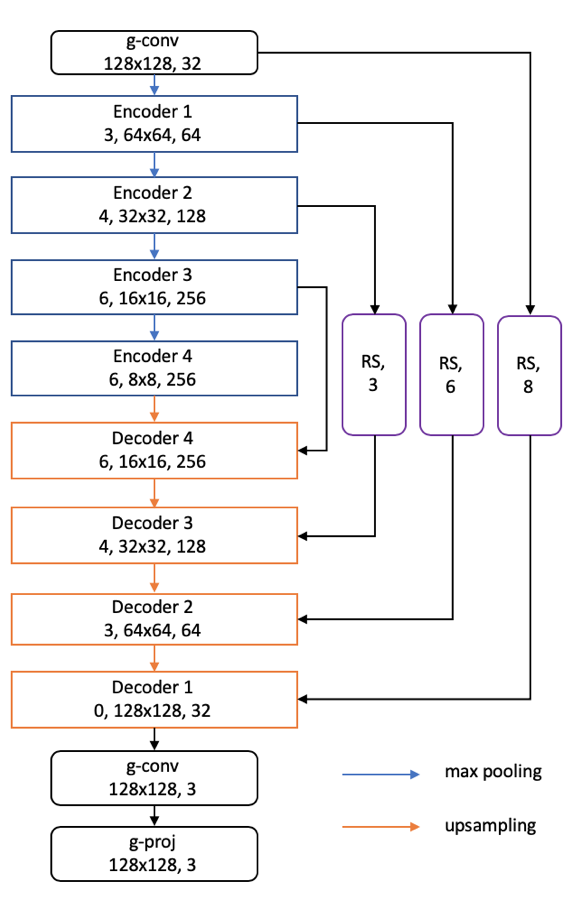
\includegraphics[scale=0.95]{resources/4_UNet_Architecture-part1.png}
    \caption{Our proposed rotation and translation-equivariant U-Net architecture at the 
    highest-level view, showing sequential encoder and decoder blocks.}
    \label{fig:g_u_net}
\end{figure}

Our residual blocks along the long-skip connections of low-level layers are also shown in Figure~\ref{fig:g_u_net_details}: (a) details of encoder blocks; (b) details of decoder blocks;     (c) details of RS blocks, with several residual blocks in series, which are found on long-skip connections and within decoder and encoder blocks; and (d) details of residual blocks. Because of limited space, we omit the visualization of batch normalization layers and ReLu activation layers after g-conv blocks. 

\begin{figure}[thb]
    \centering
    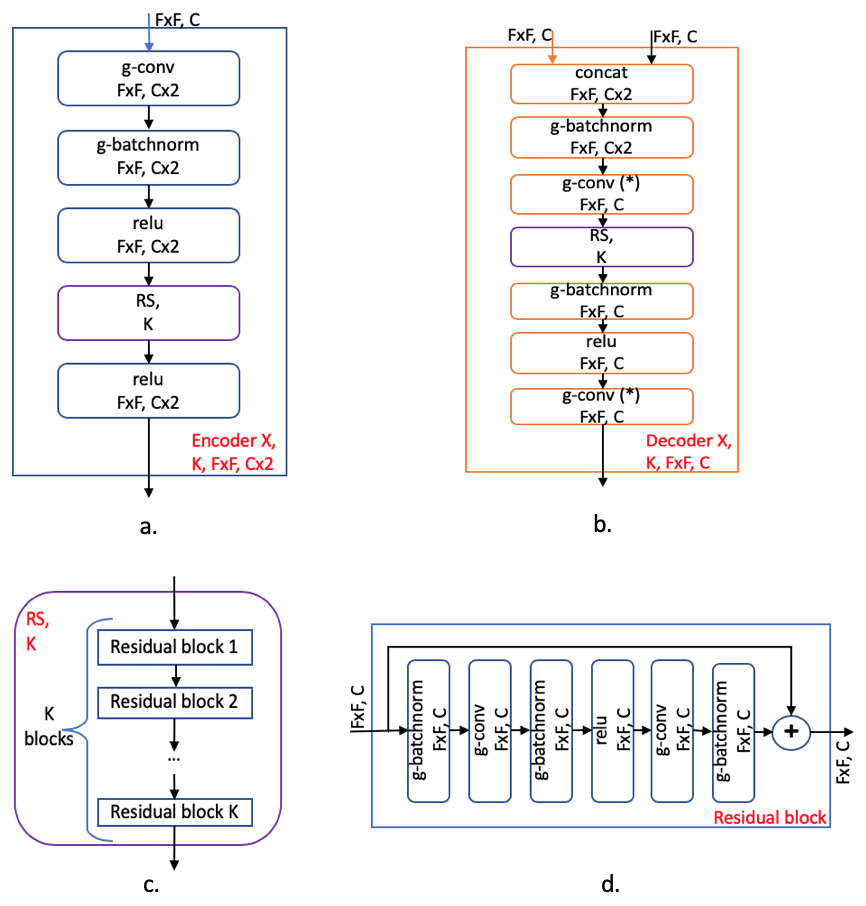
\includegraphics[scale=0.95]{resources/4_UNet_Architecture-part2.png}
    \caption{Residual blocks along the long-skip connections of low-level layers.}
    \label{fig:g_u_net_details}
\end{figure}

\subsubsection*{Group-equivariant convolution}
Group-equivariant convolution is the generalization of convolution to functions on groups, the set $\mathbb{Z}^{2}$ with translation, on which convolution is normally defined, being a specific type of group.
For a group $G$, the convolution of a filter $\psi\colon G\rightarrow \mathbb{R}^{K}$ with a feature map $f\colon G\rightarrow \mathbb{R}^{K}$  is defined to be the sum, over all elements in $G$, of their inner product:
\begin{equation}
    (f\ast \psi)(g) = \sum_{k}\sum_{h\in G} f_{k}(h)\psi_{k}(g^{-1}h).
\end{equation}
Here, the action of element $g$ on $h\in G$ is expressed by $gh$, and $g^{-1}h$ is the action of the inverse of $g$.
For example, if the group is the translation of elements $x\in\mathbb{Z}^{2}$, then $gx = x + g$ and $g^{-1}x = x - g$ and we would have standard convolution.
Since the output function is a function of $G$, which indexes not only pixel locations, but also rotations, this information can be preserved throughout the network thereby preserving equivariance to such transformations.

Since the input images to the network are functions on $\mathbb{Z}^{2}$, the output of the first group-equivariant convolutional layer is a special case, given by
\begin{equation}
    (f\ast \psi)(g) = \sum_{k}\sum_{z\in \mathbb{Z}^{2}} f_{k}(z)\psi_{k}(g^{-1}z).
\end{equation}

\subsubsection*{Group-equivariant upsampling}

For the upsampling arm of the U-Net, before each layer, we first upsample the feature map from the layer below by 2 using nearest-neighbor interpolation, which preserves equivariance to translations and rotations of 90 degress.
This method of upsampling is the same as \emph{deconvolution} or \emph{transpose} convolution with a $2 \times 2$ filter of all ones~\cite{FCNs} and helps to keep the number of trainable filters in the network manageable.
%For the upsampling arm of the U-Net, convolution is replaced with \emph{deconvolution}, or \emph{transpose} convolution.
%Deconvolution in the context of a U-Net is accomplished by first interpolating the feature map uniformly with zeros so that it is the desired dimension, and then convolving~\cite{long2015fully}.
%As noted in~\cite{linmans2018sample}, this operation maintains group equivariance for $p4m$, regardless of the stride.

\begin{figure}[thb]
\begin{center}
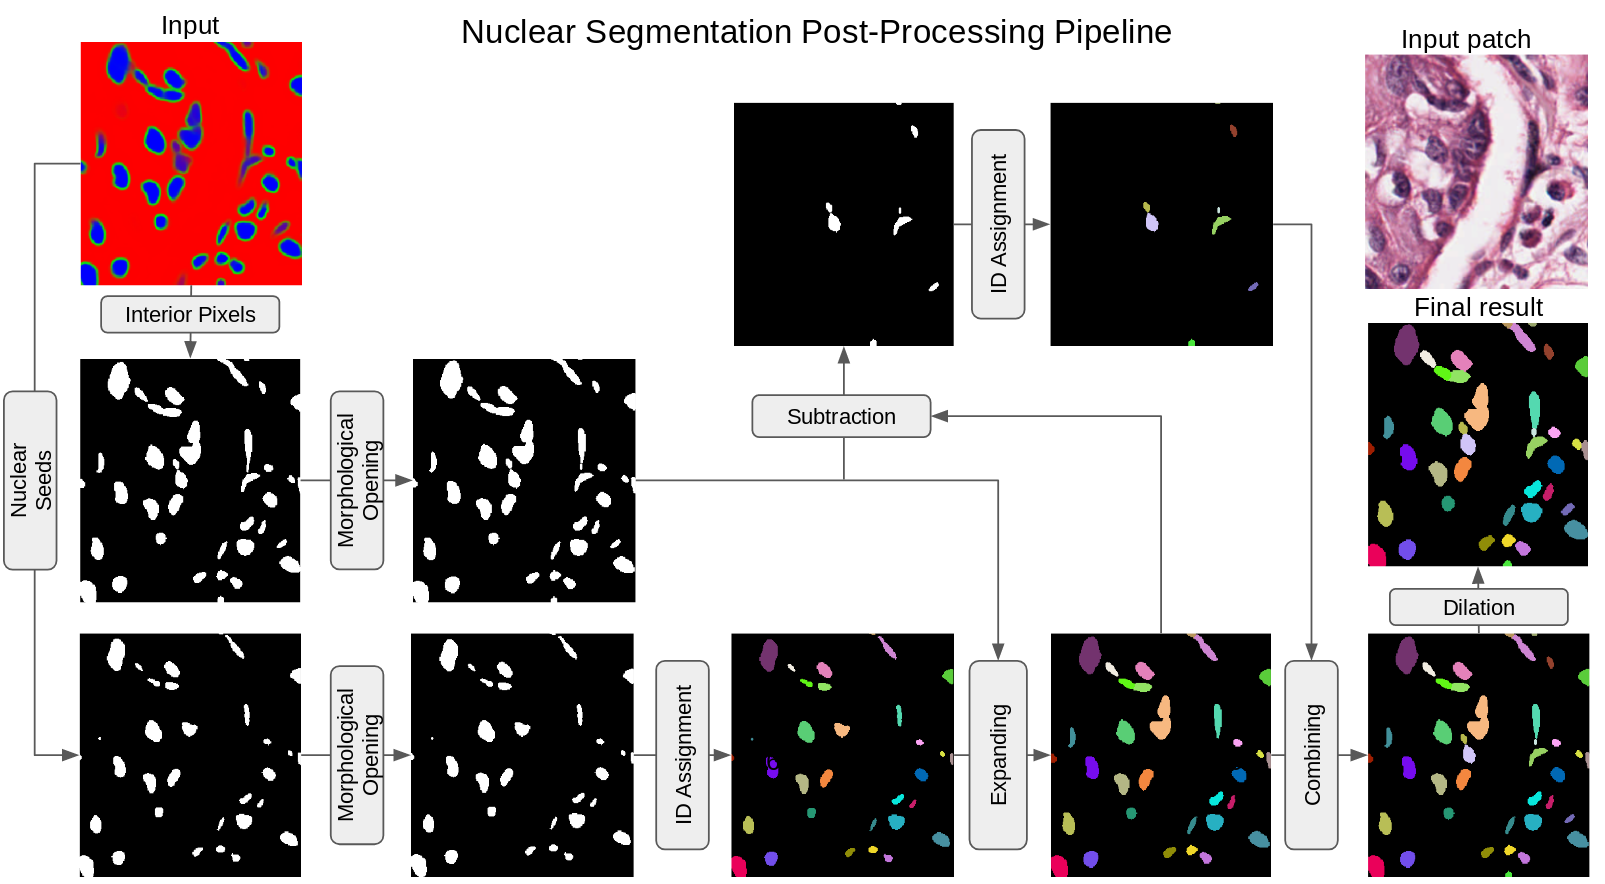
\includegraphics[width=\textwidth]{resources/4_post_processing.png}
\end{center}
   \caption{Our proposed post-processing method, consisting of a series of several morphological operations.
   Each step is visualized by its result.}
\label{fig:post_processing}
\end{figure}

\subsubsection*{Group-equivariant pooling and residual blocks}

As noted in~\cite{gcnn}, for the $p4$ group, max-pooling with a stride of 2 preserves the equivariance properties of the network, and this is the pooling operation we use in the downsampling arm of the U-Net.
Also noted in~\cite{gcnn}, since residual blocks are simply the addition of two group-equivariant feature maps, the output will also be group-equivariant.

\subsubsection*{Group projection}
To create the final segmentation image, we must transform the domain of the feature maps in the U-Net from $G$ back to $\mathbb{Z}^{2}$.
To do so, we average the feature map for each filter over rotations.
This is called the group \emph{projection} layer, as in other works~\cite{DBLP:journals/corr/abs-1807-00583}.

\subsection{Long-skip connections with residual blocks}
In the typical U-Net~\cite{unet} architecture, the number of convolution blocks at low-level layers is small, which limits the effective local field-of-view and thereby decreases the quality of features which the network can use to delineate the output boundary.
To provide richer low-level features to the final layers of the upsampling arm of the U-Net, we enhanced the baseline U-Net by adding residual blocks on long-skip connections.
Our long-skip connections enhanced with residual blocks are visualized in Figure~\ref{fig:g_u_net}a, and a detailed view of the long-skip connections and residual blocks are shown in Figure~\ref{fig:g_u_net}d and Figure~\ref{fig:g_u_net}e, respectively.

\subsection{Morphological post-processing}

Even though the U-Net deep learning architecture produces a full segmentation mask, unlike patch-based deep learning methods, post-processing, specifically morphological operations, are still essential to yielding contiguous regions and accurate nuclear boundaries.
%To aid the network in learning invariance to rotations and flips, each image is manipulated by rotations of 90 degrees and vertical flipping and the result of the network for all eight orientations is averaged to yield a single map indicating the probability of each pixel belonging to each label.
We designed a post-processing pipeline, shown in Figure~\ref{fig:post_processing}, to accomplish this.
It consists of the following steps.
A mask of confident interior pixels is created by identifying pixels for which the inside probability is greater than other labels, followed by morphological opening.
A map of nuclear seeds is created by thresholding ($thres = 0.85$) the probability of the interior class of these pixels, followed by opening.
Each seed is assigned a unique index, which is propagated to all connected interior pixels.
Regions not covered will be assigned new index and combined with the previous result.
Then, we apply binary dilation to create the final result.
The parameters, such as window size, for these various morphological operations were optimized on the validation set in our experiments.

%\begin{figure}[t]
%\begin{center}
%\includegraphics[width=0.42\textwidth]{image/img_new_synthetic_normalized_edit.png}
%\end{center}
%   \caption{Data augmentation and color normalization. The first row shows example training images from~\cite{kumar2017dataset}.
%   The second row shows synthetic images generated by our proposed data-augmentation method.
%   %New shape and orientation of nuclei eyes generated along with translation, which increases the overlapping rate, make the training set more diverse. These new synthetic images have a significant contribution to the performance. 
%   The last row shows the original training images normalized by method proposed in~\cite{7164042}. \CC{[TODO: merge with Figure 4]}} 
%   %By converting all images to one color space, we can reduce the color variance problem, which alleviates the challenge when the model is trained.}
%\label{fig:data_visualize}
%\end{figure}
%

\begin{figure}[thb]
    \centering
    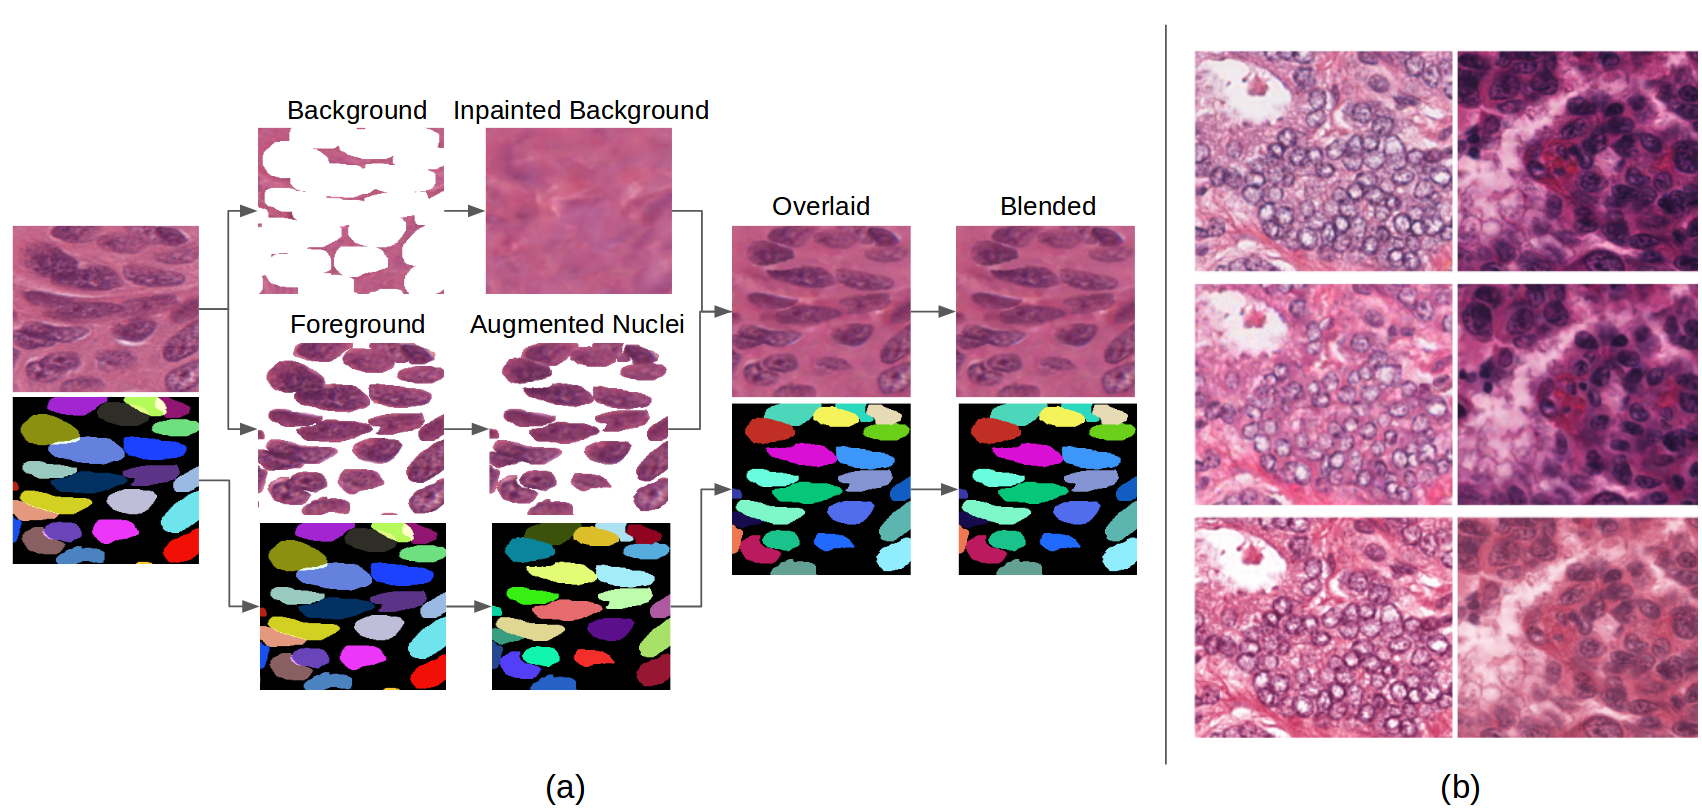
\includegraphics[width=\textwidth]{resources/4_data_augmentation.png}
    \caption{(a) Our proposed process generating new synthetic images with their corresponding annotations. 
    (b) Data augmentation and color normalization examples.
    The first row shows example training images from~\cite{he_dataset_kumar}.
    The second row shows synthetic images generated by our proposed data-augmentation method.
    %New shape and orientation of nuclei eyes generated along with translation, which increases the overlapping rate, make the training set more diverse. These new synthetic images have a significant contribution to the performance. 
    The last row shows the original training images normalized by the method proposed in~\cite{7164042}.
    %By converting all images to one color space, we can reduce the color variance problem, which alleviates the challenge when the model is trained.}
    }
    \label{fig:generate_new_data}
\end{figure}

\subsection{Data augmentation by nuclear deformation}

To aid in training a robust network that minimizes overfitting, we implemented a novel approach designed specific for histology image analysis to generate augmented training images.
Given the ground-truth annotations, each nucleus in an image is extracted and then deformed slightly by affine, spline, and elastic transformations as well as small random translation, yielding a new orientation, position, and shape.
Extracting the nucleus from the image produces empty holes in the background, which are filled by the image inpainting method proposed in~\cite{DBLP:journals/corr/abs-1801-07892}.
Some elastic transformations and slight Gaussian blurring are applied at this point, along with some added speckle noise.
The transformed nuclei are then overlaid back onto the reconstructed background image.
%We found that the signals of these cells are already smooth, so we do not need any blending method when placing these cells back to new background.
Finally Gaussian blurring is applied to help smooth any harsh or unnatural edges between the augmented nuclei and the background.
Figure~\ref{fig:generate_new_data} diagrams this process and shows examples of resulting augmented training images. 

\subsection{Stain normalization}
To reduce the uninformative and possibly confusing color variation inherent to H\&E stained images, we use the structure-preserving color normalization method proposed in~\cite{7164042}.
One image from the training data set is used as the target and all other images, including the new augmented data, are converted to its color space.
We use $\lambda = 0.1$ as recommended in~\cite{7164042}.
The last row in Figure~\ref{fig:generate_new_data}b shows example normalized images.


\begin{ChapAbstract}
In this chapter, we discuss the main challenges not only in nuclear segmentation but also other related domains such as astronomy analysis, video object segmentation. Moreover, we also describe the merit of our enhancements to overcome mentioned challenges, which can be extend to solve these problems in other fields.
\end{ChapAbstract}

% \chapter{Experimental Results of abnormalities findings and landmark detection for endoscopic images}
\label{chap-experiment-endoscopy} 
\begin{ChapAbstract}
In this chapter, we describe the dataset, task descriptions as well as the evaluation metrics used in both following challenges: The 2018 Multimedia for Medicine Task and and The Biomedia ACM MM Grand Challenge 2019. We not only report our official results provided by organizers but also discuss about the performance of each component in our algorithm by trying different experiment configurations and analyze the corresponding results.
\end{ChapAbstract}

\section{Dataset and evaluation metrics}
\label{dataset_evaluation_endoscopy}
\subsection{Dataset}
\subsubsection*{Dataset description}
According to organizers of The 2018 Multimedia for Medicine Task, the offical dataset contains a multi-class set of frames and videos for at least 4 different diseases, at least 4 different landmarks and at least 2 different findings. Each class will consist of at least 1000 frames and at least 2 short videos. The training set will be released with ground truth. All the frames in training set will be labelled with corresponding class-label. Up to 10\% of training set frames will have a detailed ground truth masks showing the exact location of disease or finding within the frame. The ground truth is collected with the help of GI endoscopists from our partner hospitals. The pre-extracted visual features such as global image features, namely: JCD, Tamura, ColorLayout, EdgeHistogram, AutoColorCorrelogram and PHOG are also included in this dataset.

\subsubsection*{Classes}
Totally, there are 16 classes of abnormal symptoms and landmark of human's gastrointestinal track (GI track). The visualisation of landmark's corresponding position in the GI track are shown in Figure \ref{fig:vis_16_classes}. As given  in the figure, the \textit{esophagitis, normal z-line, normal  pylorus, ulcerative colitis, colon, normal cecum, retroflex-stomach, retroflex-rectum and stool (plenty/inclusion)} are classes which illustrate the landmark in human's GI Track. Noticeably, the \textit{esophagitis} and \textit{normal z-line} share a same anatomical position. However, the class \textit{esophagitis} (marked with a red bounding box) refers to an  abnormal situation and \textit{normal z-line} (marked with a green bounding box) appears in normal people's GI track. Similarly, the \textit{ulcerative colitis} (marked with a red bounding and \textit{colon} (marked with a green bounding box)  refer to an abnormal and a normal situation respectively.

Besides, the \textit{dyed-lifted-polyps, dyed-resection-margins, polyps} and \textit{instruments} are abnormal symptoms that can be appeared at any position in the human's GI track. In addition, the \textit{polyp} is a  living entity in the GI track, doctors can inject some chemical component in order to demolish polyps. This chemical changes polyp's color to white, which became the \textit{dyed-lifted polyps}. After that, doctors will use some special \textit{instruments} to remove the polyp completely, the remains are \textit{dyed-resection-margins}. 

\begin{figure}[thb]
\begin{center}
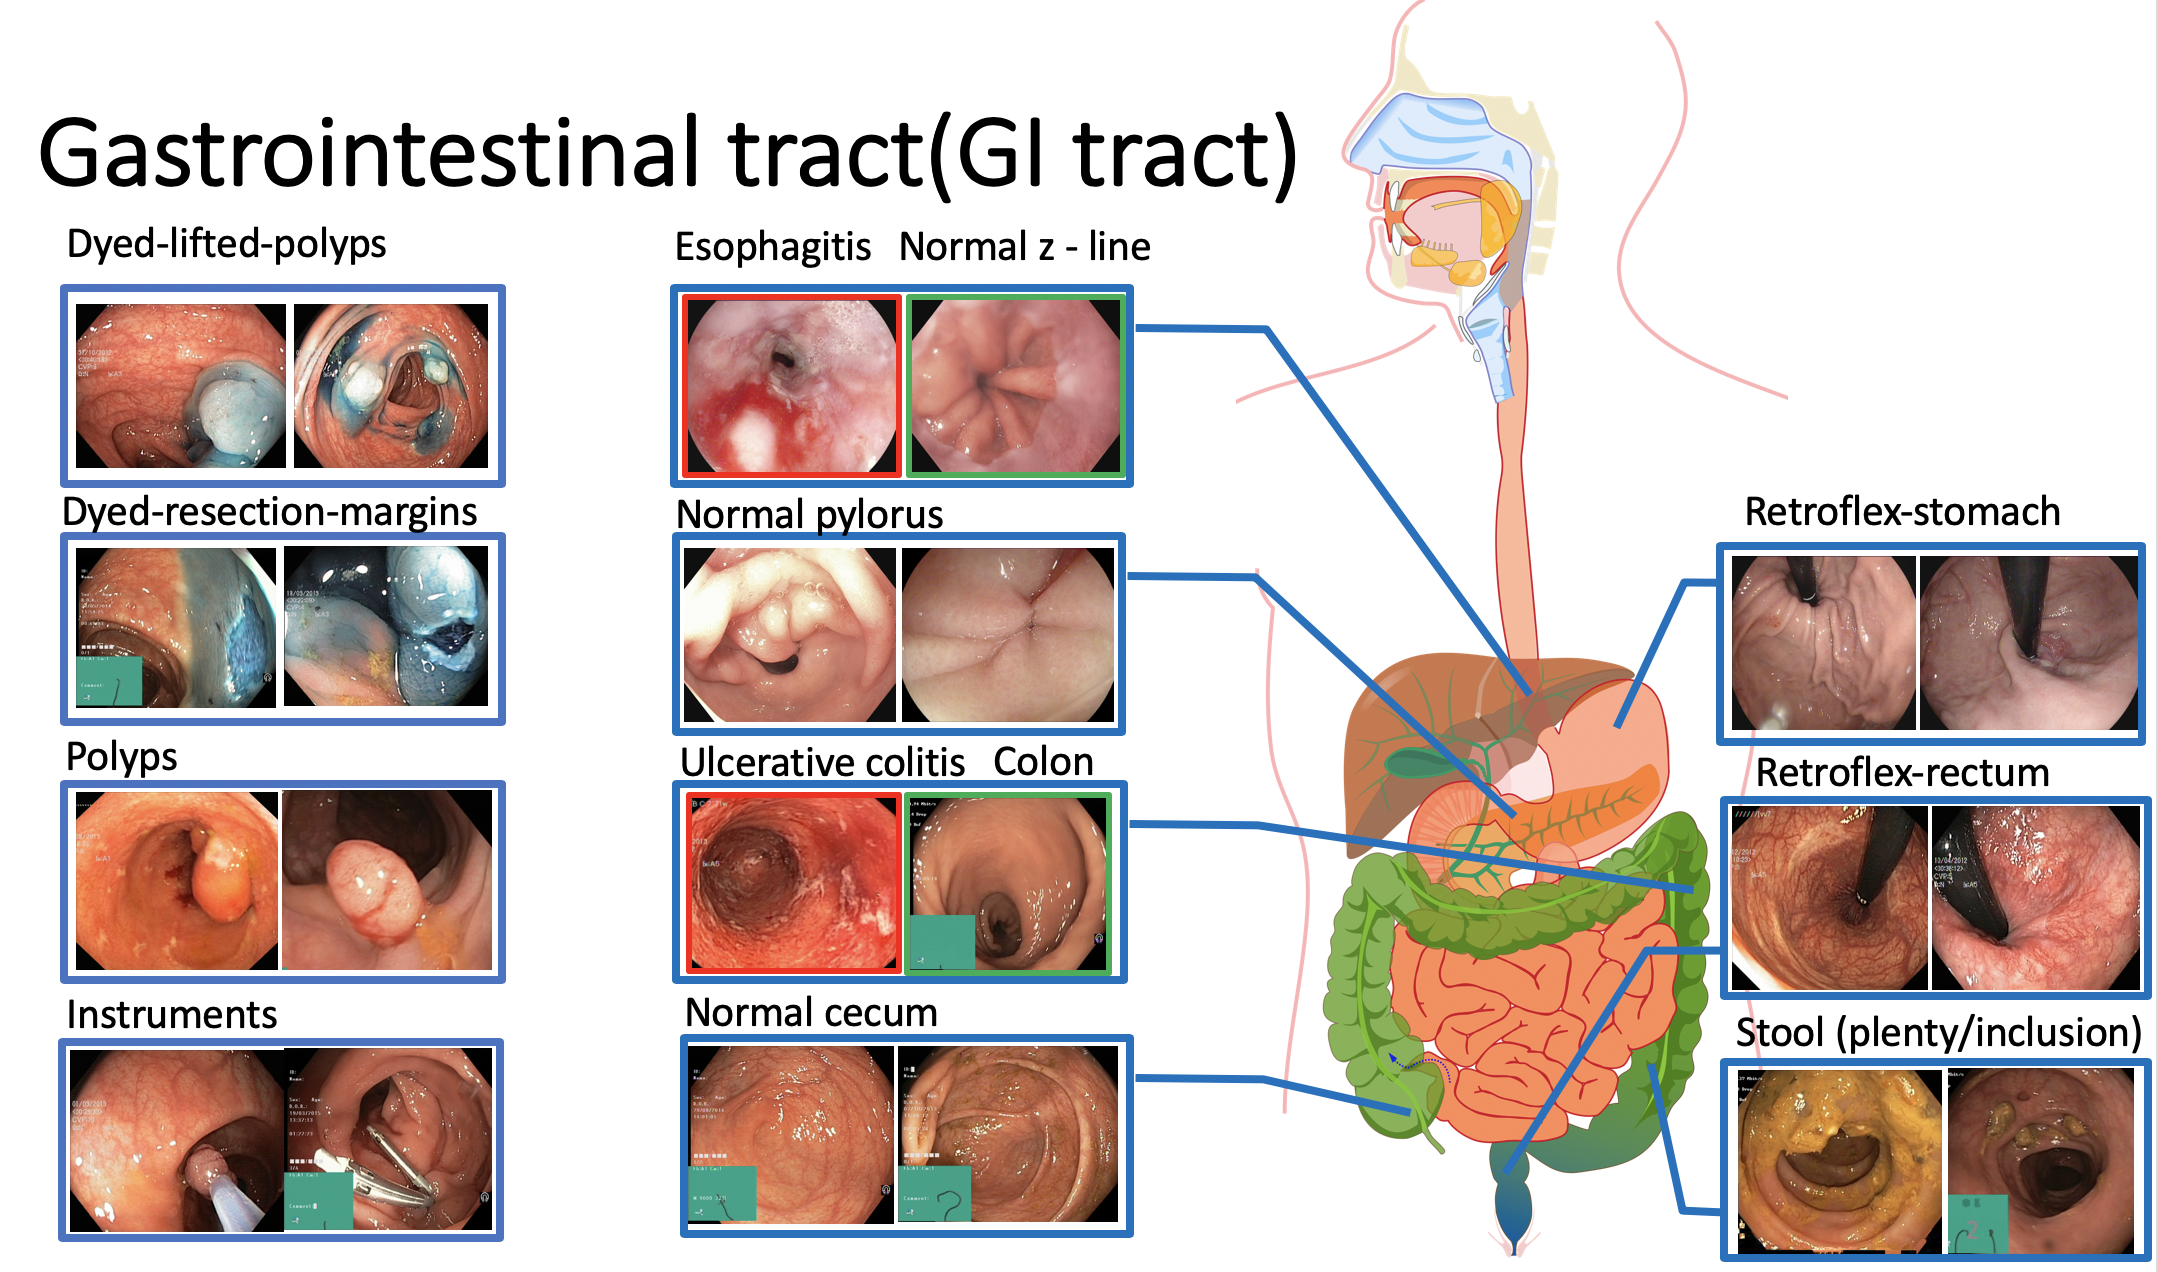
\includegraphics[width=\textwidth]{endoscopy_resources/vis_16_classes.png}
\end{center}
   \caption{Classes of the Medico: The 2018 Multimedia for Medicine Task official dataset and their corresponding order in the Gastrointestinal track.}
\label{fig:vis_16_classes}
\end{figure}

\subsubsection*{Multi-classes classification}
When we conducting our experiments on this dataset, we find out that both the development set and the test test contain a number of images can be classified into several classes simultaneously. After noticing the task organizers for this problem, they define a priority list according to the important level of that finding during the endoscopy screening process. The list is given bellow in descending important level (most important to less important):

\begin{multicols}{3}
\begin{enumerate}
    \item out-of-patient
    \item instruments
    \item dyed-lifted-polyps
    \item dyed-resection-margins
    \item polyps
    \item esophagitis
    \item ulcerative-colitis
    \item retroflex-rectum
    \item retroflex-stomach
    \item normal-cecum
    \item normal-pylorus
    \item normal-z-line
    \item stool-plenty
    \item stool-inclusions
    \item colon-clear
    \item blurry-nothing
\end{enumerate}
\end{multicols}

\subsubsection*{Development Set and Test Set}
In this challenge, task organizers divide this 16-classes dataset into two sub-set: \textit{the development set} consists of 5293 images  and the  \textit{test set} consits of 8740 images. Only the image's label of the \textit{development set} are visible to participants.

\subsection{Evaluation metrics}
Regarding to the evaluation process, task organizers propose several metrics for each sub-task. Totally, there are four sub-tasks can be conducted on this dataset, including \textit{Classification of diseases and findings}, \textit{fast and efficient classification}, \textit{basic reporting} and \textit{advance reporting}. In our work, we evaluate our approaches on the first and the second sub-task. The remain sub-tasks are not conducted by our team or others and they are left for future development.
\begin{itemize}
    \item \textbf{Classification of diseases and findings:} The evaluation metric is the multiclass version of the Mathews Correlation Coefficient (MCC) \cite{MATTHEWS1975442}, which captures the quality of classification as reflected in the correlation between the ground truth and the classifier's predictions. The MCC can be calculated directly from the confusion matrix using the formula:
    \begin{equation}
        MCC = \frac{TP \times TN - FP \times FN }{\sqrt{(TP + FP)(TP + FN)(TN + FP)(TN + FN)}}
    \end{equation}
        
    where $TP$ stands for the number of true positives, $TN$ is the number of true negatives, $FN$ is the number of false negatives and $FP$ is the number of true negatives.
    \item \textbf{Fast and efficient classification:} Participants of this sub-task are asked to run the code on a standard PC and provide information about hardware used. The time from input to output will be measured and weighed by the accuracy of the output. Participants are also asked to record the amount of training data used. The amount of training data will also be weighted by the accuracy of the output.
    \item \textbf{Reporting (exploratory/optional):} The metric will reflect the completeness and the correctness of the summary. This sub-task allows organizers to focus on understanding the performance of the automatic systems in practice (from the point of view of the medical expert). However, this sub-task is currently an optional sub-task.

    \item \textbf{Advanced reporting (exploratory/optional):} In order to evaluate participant's result on this sub-task, two medical partners will participate in the evaluation process in terms of how useful it is for them and if it satisfies existing demands for documentation of endoscopic procedures. Similar to  the above sub-task, this sub-task is also an optional sub-task.
\end{itemize}

\section{Experimental setup} 
\label{sec:endscopy_setup}
\subsection{Re-labeling Medico Development Dataset}
After training with the development set of Medico 2018 challenge, we find some issues related to some training samples in the given dataset. Firstly, with a help of a medical student, we found out that there are inappropriate labels according between different classes. Secondly, there are several samples in the development set that conflict with the priority list that the organizers proposed. Therefore, in order to help our model to learn with the least confusing, we apply the new labels and make them as the modified version of the original dataset. We also make that modified version of the given dataset available to be contributed for the task organizers in future challenges. 

\subsection{Abnormalities localization with Faster R-CNN}
We inherited the work from Chen et al. \cite{chen17implementation} which is a Tensorflow implementation of faster RCNN detection framework. Due to the small size of abnormalities in endoscopic image dataset, we use several anchors size at $4,8,16,32$ and corresponding aspect ratios at $0.5,1,2$. ResNet 101 pre-trained model \footnote{\url{github.com/tensorflow/models/tree/master/research/slimơ\#pre-trained-models}} is used as Faster R-CNN backbone. The concepts we used to train including \textit{instruments, polyps, dyed-lifted-polyps} and \textit{dyed-resection-margins}. Original and our augmented dataset are trained simultaneously for 70000 iterations. It usually takes 5-6 hours training on GeForce GTX 1080 GPU.

In test-time inference, each image is fed through the module and we only keep bounding boxes that have confident score over $0.95$.

\subsection{ResNet Classifier and Multi-tasks Classifier}
Classifiers used in our work are implemented with PyTorch - a Python machine learning library. Original and our augmented dataset are trained simultaneously for 200 epochs with Adam optimizer \cite{DBLP:journals/corr/KingmaB14}. The learning rate is set at $10^{-3}$ and decay by a factor of $0.1$ every $10$ epochs. When training the model, we freeze every layer except the last convolution and fully connected layer. In training phase, each image is resized into a batch of 64 images with size $224\times224$ are fed into the network at each step. We also apply random horizontal flip and random crop augmentation during this phase. 
\section{Experimental results}
\subsection{Abnormalities localization with Faster R-CNN results}
According to our experiments, applying object detection model such as Faster R-CNN shows significant improvements in two situation:
\begin{itemize}
    \item In the first situation, abnormal symptoms appeared in small regions of an image, that can be easily mis-classified by the image classification module. This situation usually happens with the \textit{instruments} class. Three examples are given in Figure \ref{fig:res_frcnn_instr} where \textit{instruments} appeared in really small region at the corner of an image.
    \item In the second situation, multiple abnormal symptoms seem to appeared together in the same image. Figure \ref{fig:res_frcnn_dyed} illustrated this situation where \textit{dyed-lifted-polyps} and \textit{dyed-resection-margins} symptoms appeared together. By having information about every symptom and their position inside an image, it is easier for the system to fit with the priority list of this challenge. Besides, it also an useful source of information for future endoscopy diagnosis system that can localize the position of abnormal symptoms for doctors.  
\end{itemize} 

\begin{figure}[thb]
\begin{center}
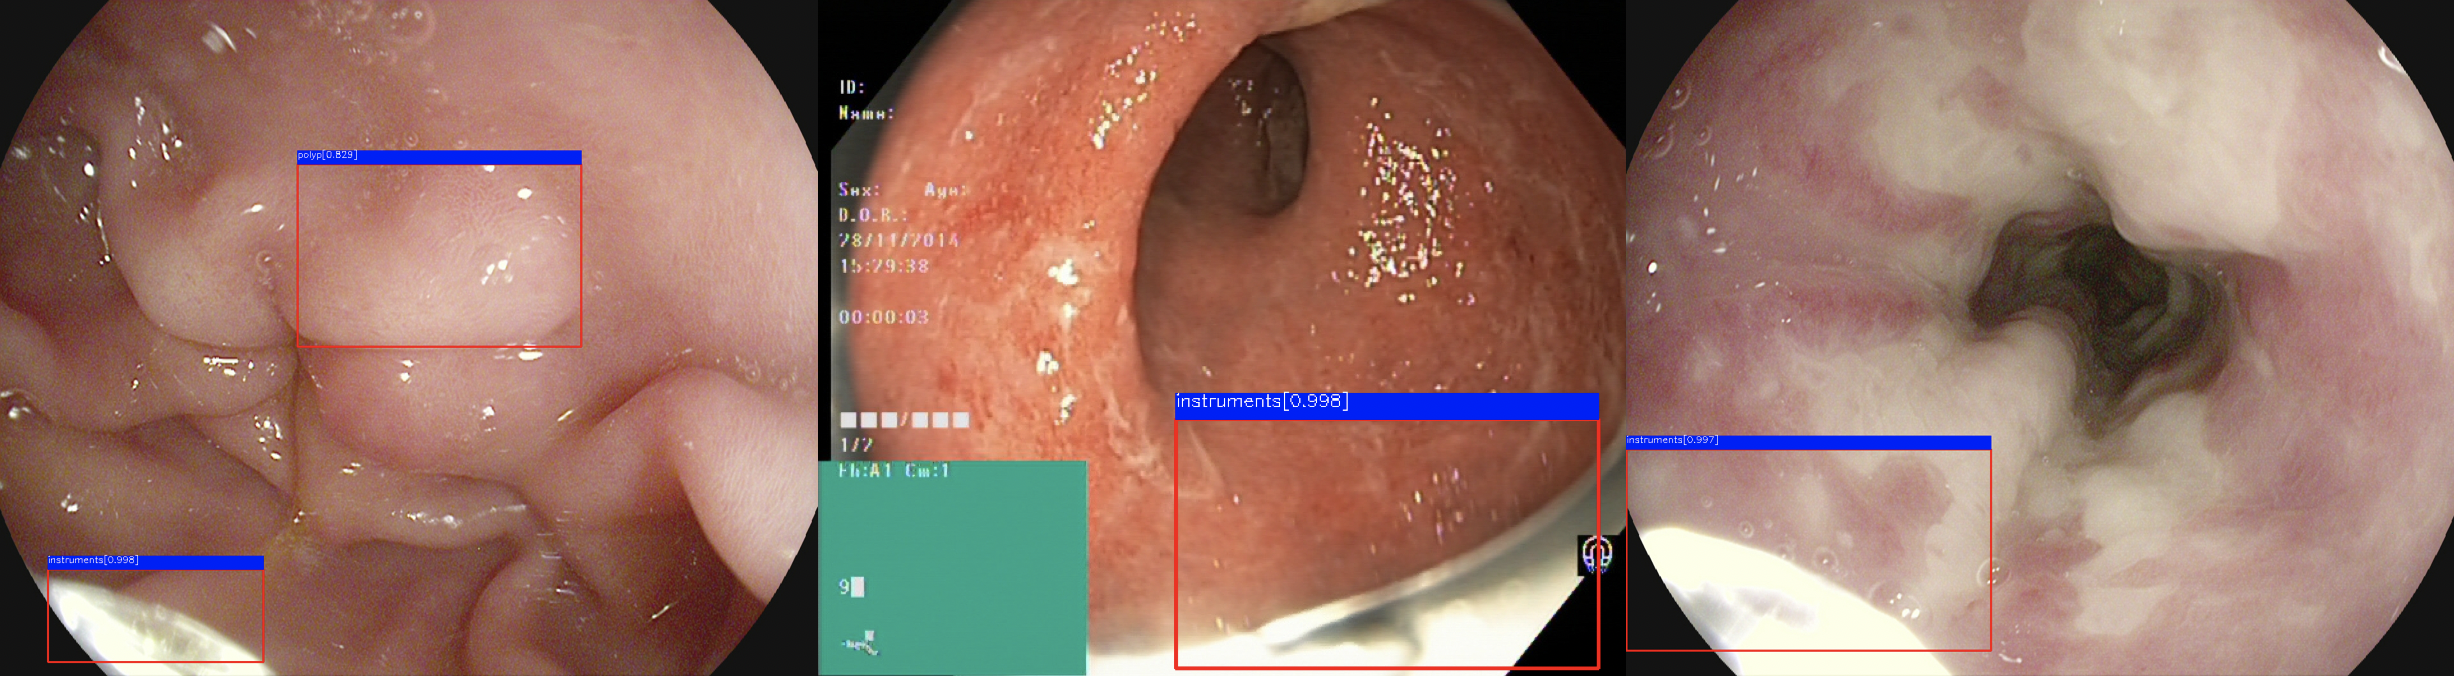
\includegraphics[width=\textwidth]{endoscopy_resources/res_frcnn_instr.png}
\end{center}
   \caption{\textit{Instrument} objects detected in endoscopic images. They are used to be mis-detected by image classification model which usually focus on global visual features.}
\label{fig:res_frcnn_instr}
\end{figure}

\begin{figure}[thb]
\begin{center}
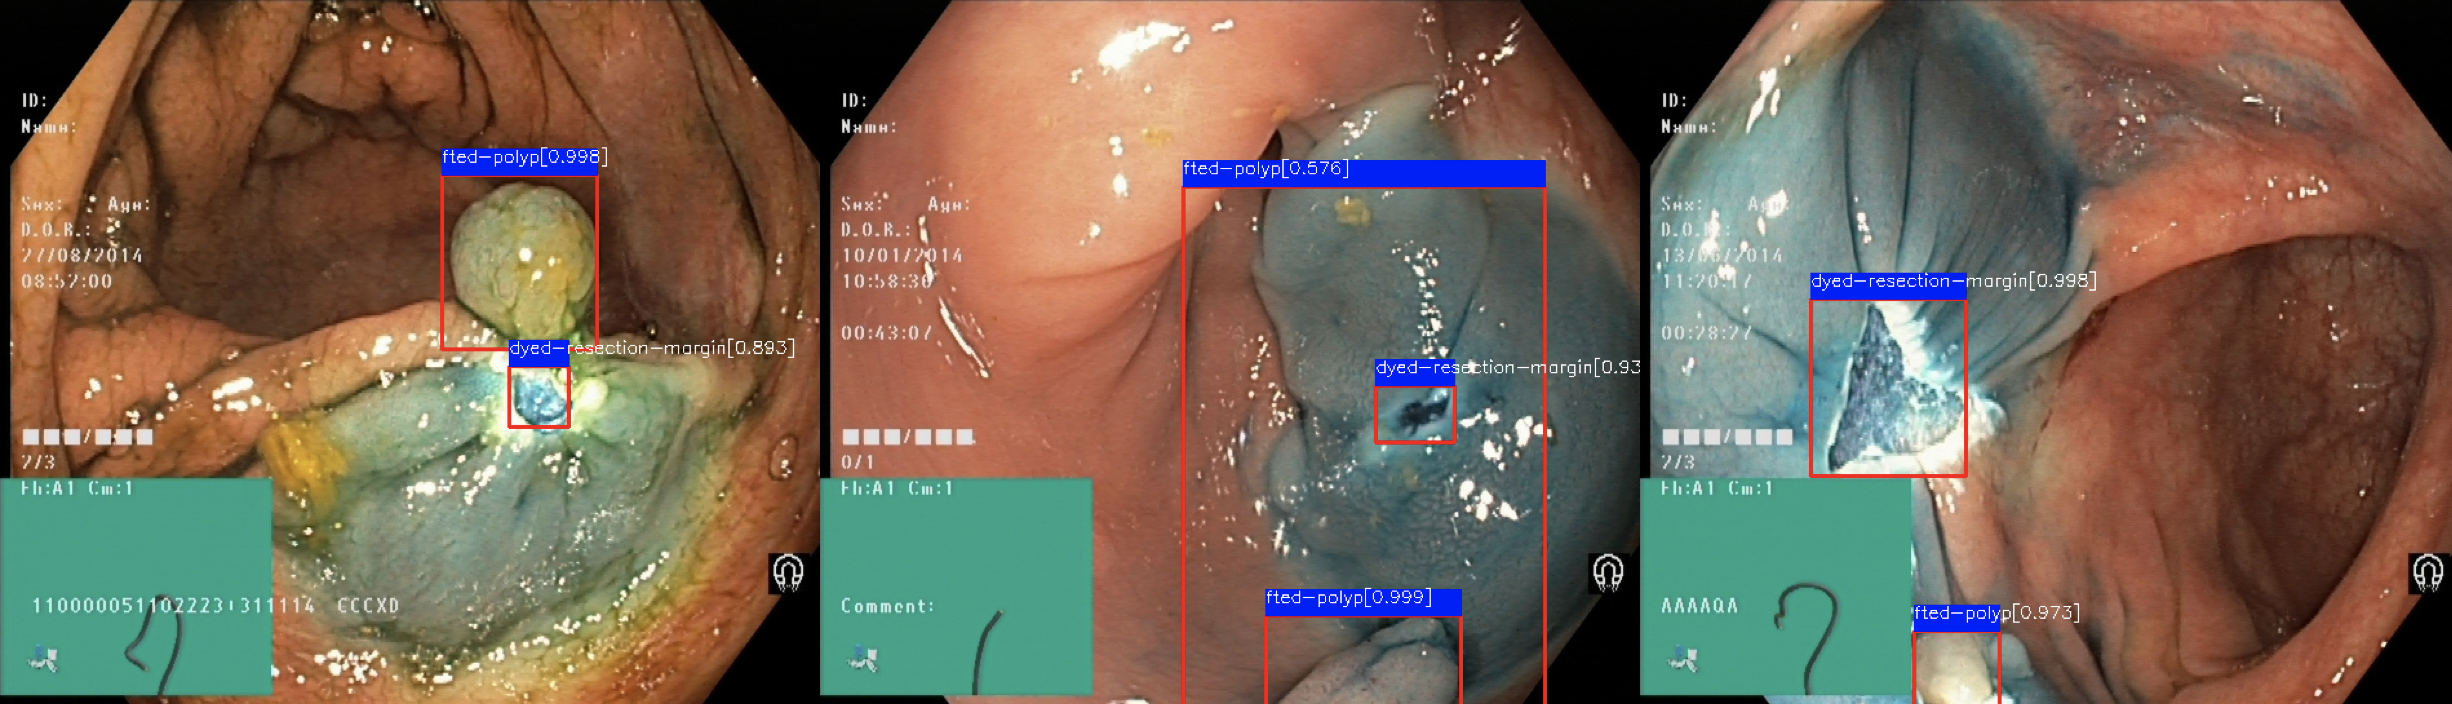
\includegraphics[width=\textwidth]{endoscopy_resources/res_frcnn_dyed_lifted_polyps.png}
\end{center}
   \caption{\textit{Dyed-lifted-polyps} and \textit{dyed-lifted-margins} symptoms detection.}
\label{fig:res_frcnn_dyed}
\end{figure}

\subsection{Medico: The 2018 Multimedia for Medicine Task - Official results}
\label{sec:medico2018_results}
Two out of three our improvements are used in the Medico: The 2018 Multimedia for Medicine Task challenge including applying object detection model on abnormal findings and dataset augmentation. Table \ref{teams_result} shows the official results of the international challenge. We received the first place winner among 10 teams around the world with the MCC score at 94.24\% and 99.33\% in term of the accuracy.

There is a trade-off between speed and accuracy when comparing the result of \textit{Run01} and \textit{Run02}. In \textit{Run02}, we reduce a large number of images passing through Faster R-CNN for the sake of time, so its performance seems to be relatively worse than \textit{Run01}'s.

As we mentioned earlier, data pre-processing takes an important role in building a deep-neural network model. Through our experiments, in the case of less training data, the augmented dataset helps us improve the performance of deep-neural network model. \textit{Run03} and \textit{Run05} show impressive results comparing to the first two runs. This implies that training on our re-labeled development set provides better models.

On the other hand, using the Residual neural network cannot classify efficiently the two classes \textit{esophagitis} and \textit{normal-z-line}. The same problem also occurs between the \textit{dyed-resection-margins} and \textit{dyed-lifted-polyps} classes. It can be observed in the confusion matrices of the two pairs (Figure \ref{fig:cfs_mat}). Therefore, these are the two main reasons which mainly bring negative impact to our results. In Figure \ref{fig:confusing}, selected samples from \textit{esophagitis} and \textit{normal-z-line} are given in order to illustrate the fine-grain situation of these classes that is challenging even for human without special knowledge to distinguish them correctly.

\begin{figure}[thb]
\begin{center}
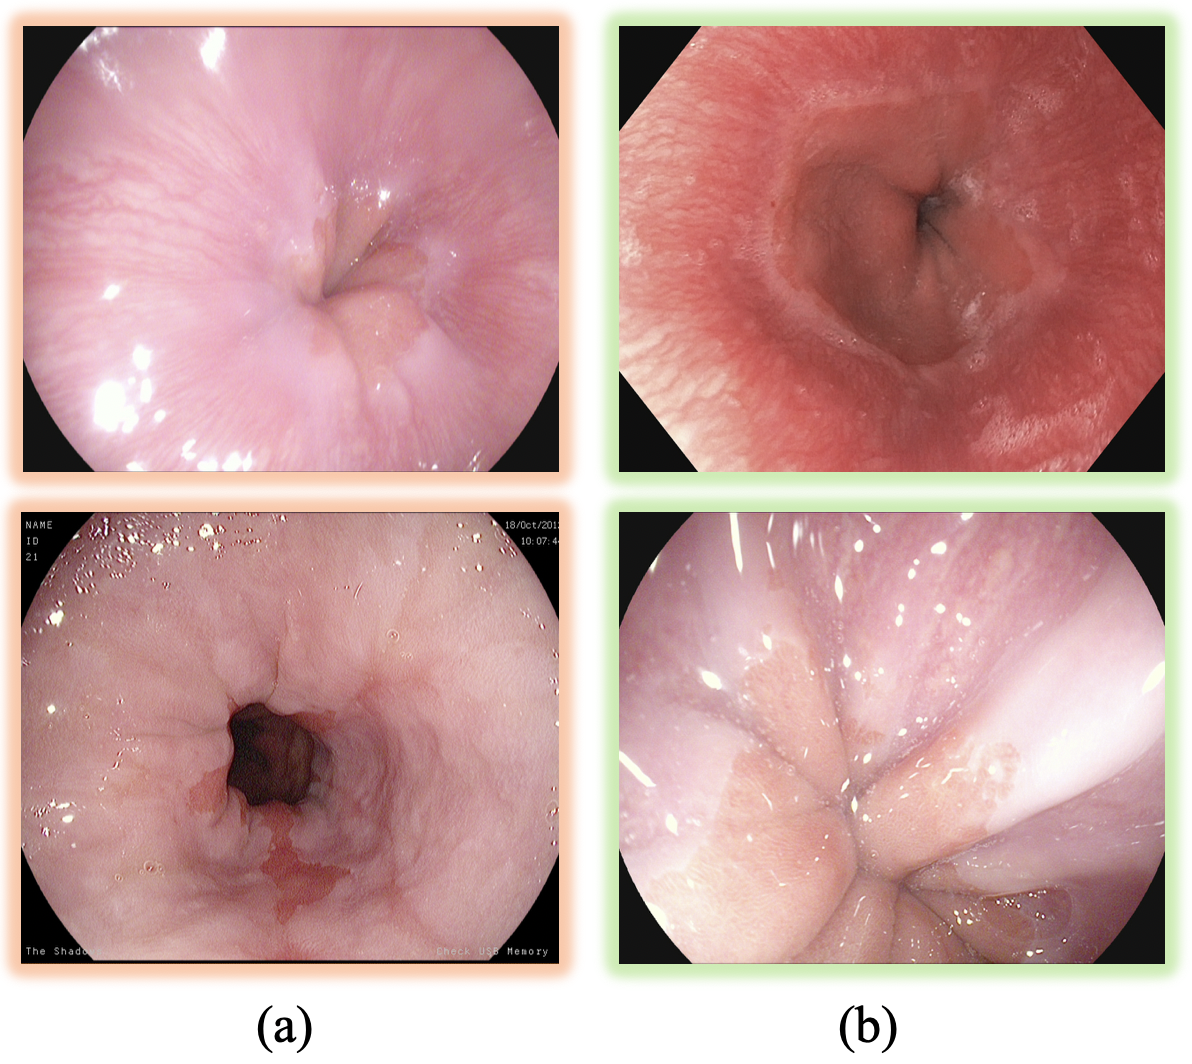
\includegraphics[width=0.8\textwidth]{endoscopy_resources/confusing_cases.png}
\end{center}
   \caption{Example of confusing cases taken from the Development Set (ground-truth provided). \textit{esophagitis} samples are marked with red box and \textit{normal-z-line} samples with green box. Two samples from the first row are harder to be distinguished than those in the second row}
\label{fig:confusing}
\end{figure}

Additionally, as we mentioned in section 3, the configuration of Run05 intuitively prefers \textit{esophagitis} to \textit{normal-z-line}, which may leads to an increasing of the false-positive cases in the result.

By comparison to the others, \textit{Run04} has the lowest precision since it uses 75\% of training data. Decreasing the amount of training samples of course affects the performance in deep-learning models. Nevertheless, the result is still acceptable when it decreases only a few percentages and its configuration is as same as \textit{Run03}. This is an evidence that we are even able to reduce up to 50\% of data when the less training time is preferred over the accuracy.

Last but not least, we performed training and testing our model on a Tesla K80 GPU. The average inference time for all images in the test set we measured for Run01 is around 150ms per image and around 43ms for others. 

\begin{figure}[thb]
\begin{center}
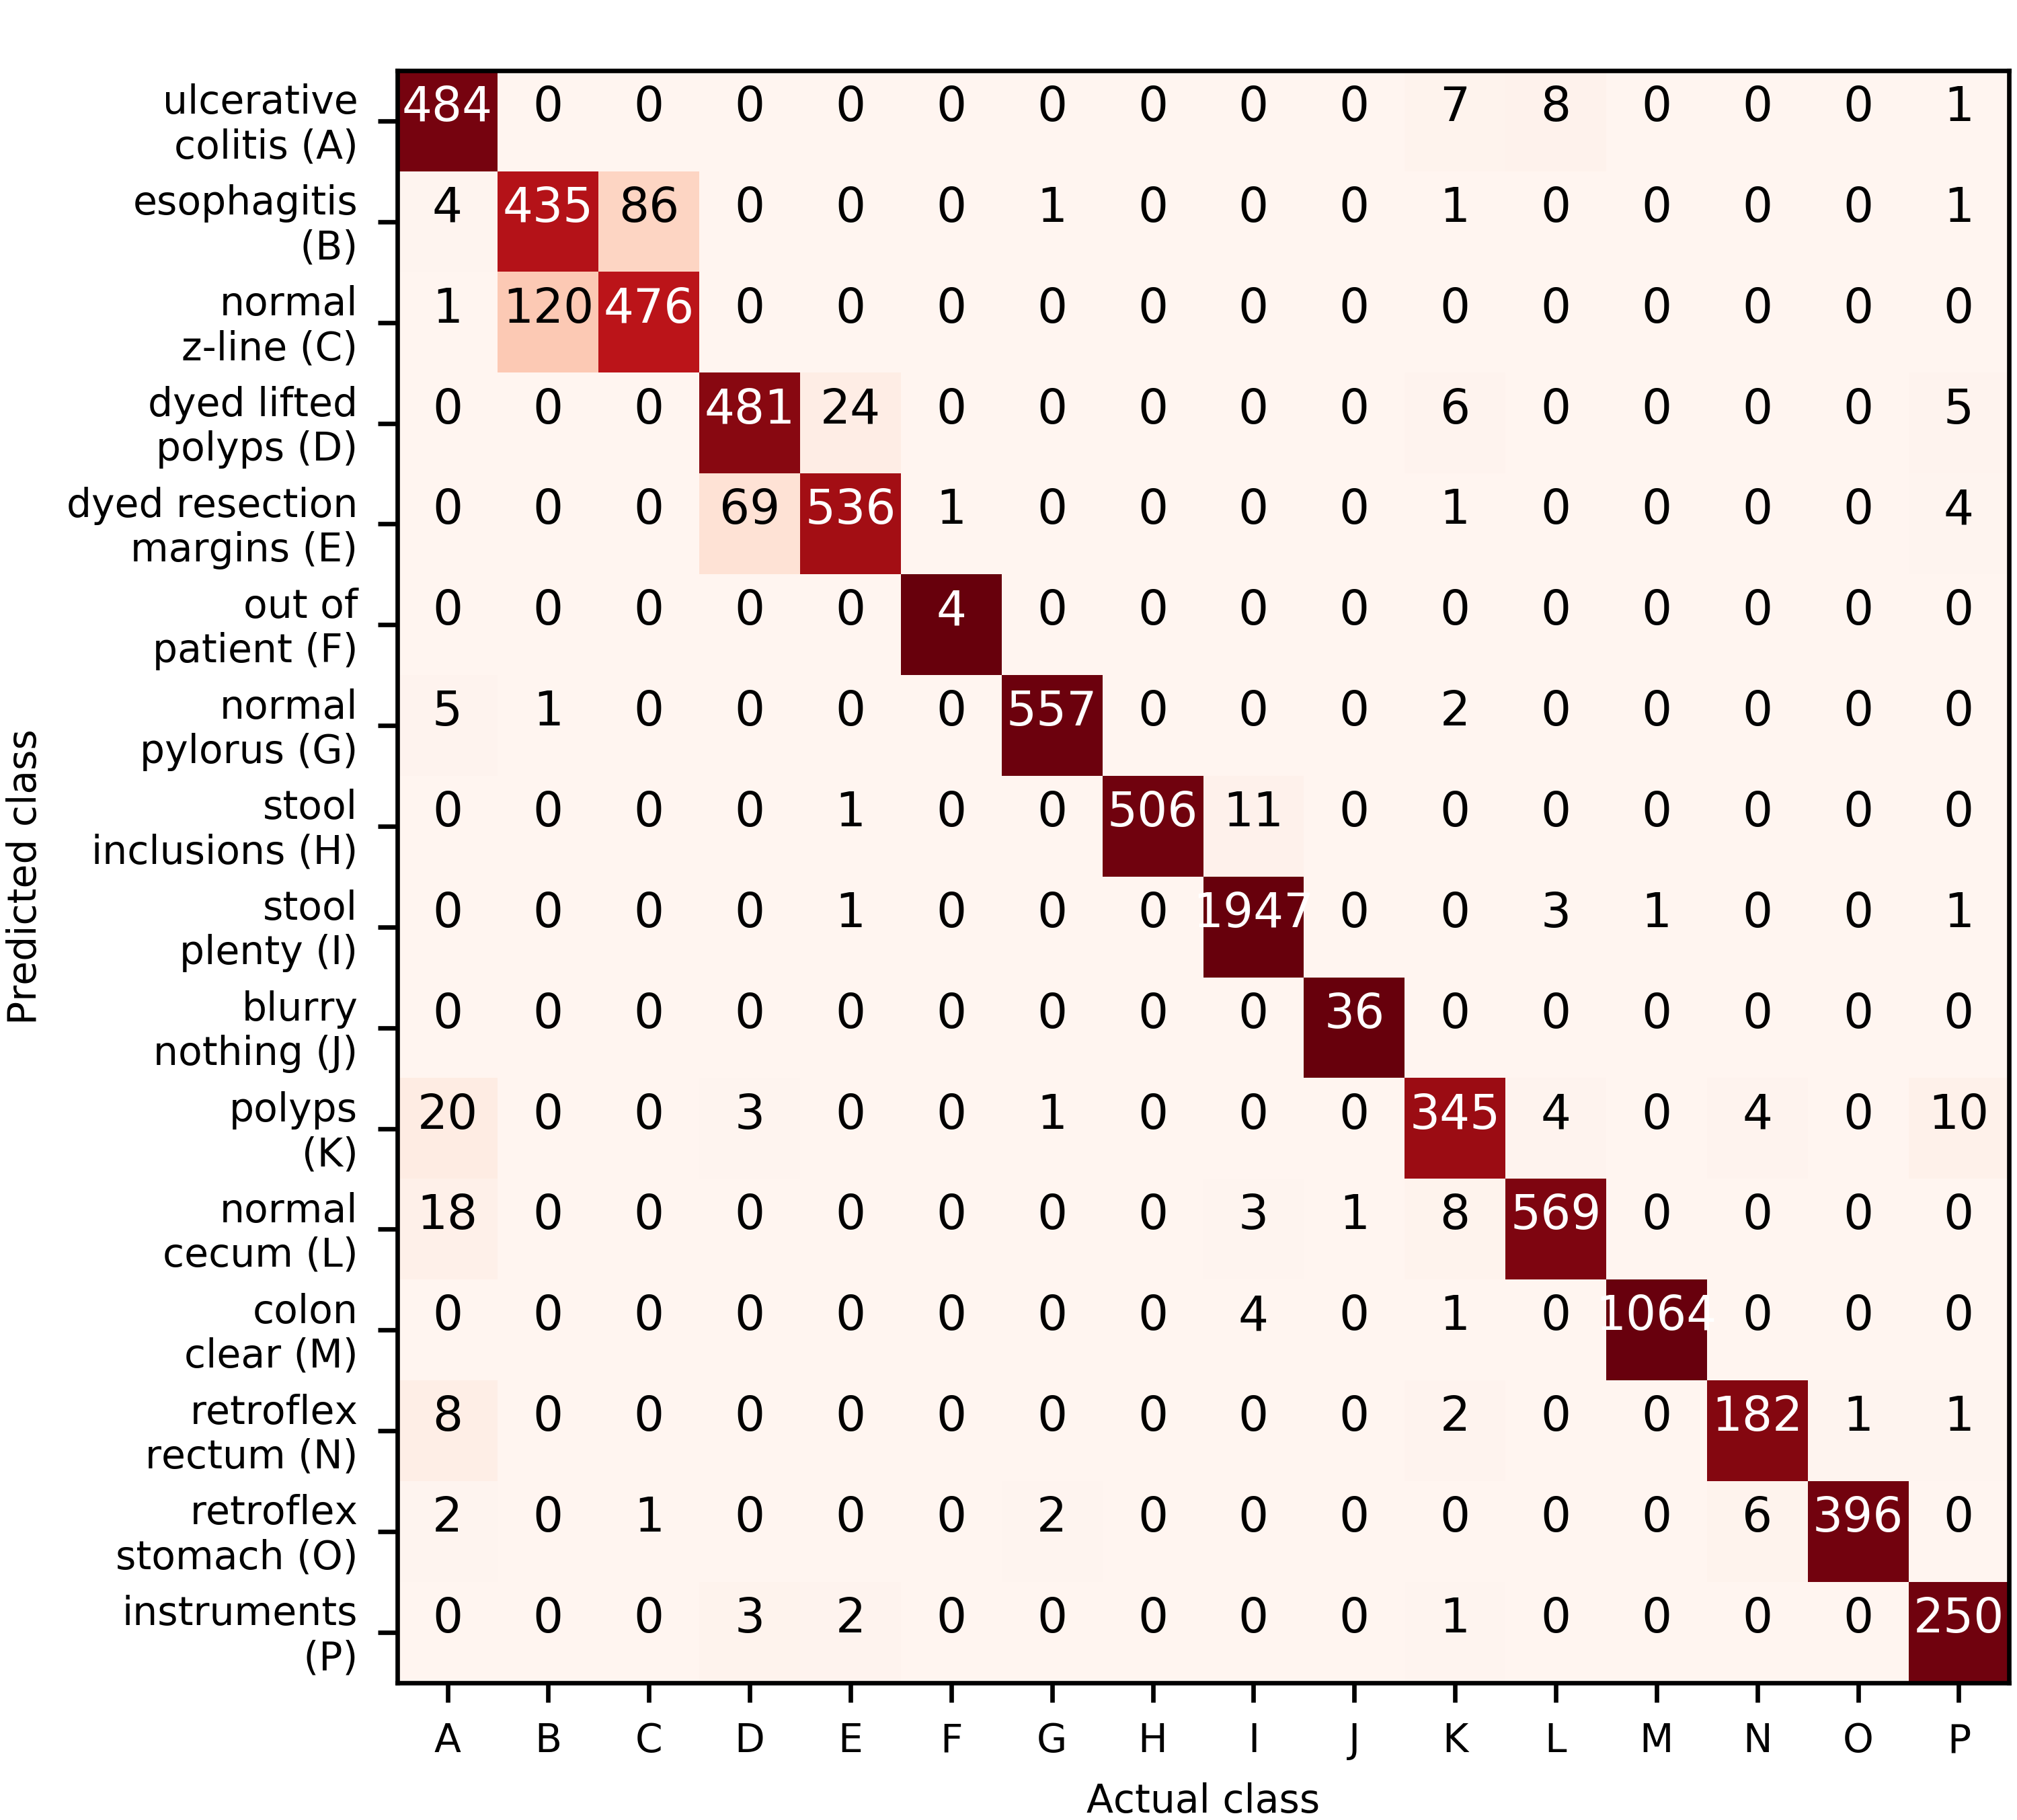
\includegraphics[width=0.8\textwidth]{endoscopy_resources/mediaeval_cfm_run3.png}
\end{center}
   \caption{The confusion matrix of our best run - \textit{Run03}.}
\label{fig:cfs_mat}
\end{figure}

\begin{table}[H]
    \caption{The official evaluation result of HCMUS team for both sub-tasks (provided by the organizers) and speed (fps) on Tesla K80 GPU}
    \centering
    \small
    \resizebox{1.0\linewidth}{!}{
    \begin{tabular}{|c|c|c|c|c|c|c|c|}
        \hline
        RunID&PREC&REC&ACC&F1&MCC&RK&FPS\\
        \hline
        Run01&94.245&94.245&99.281&94.245&93.861&93.590&6.589\\
        Run02&93.959&93.959&99.245&93.959&93.556&93.273&\textbf{23.191}\\
         \textbf{Run03}& \textbf{94.600}& \textbf{94.600}& \textbf{99.325}& \textbf{94.600}& \textbf{94.240}& \textbf{93.987}& 23.148\\
        Run04&93.043&93.043&99.130&93.043&92.579&92.257&22.654\\ 
        Run05&94.508&94.508&99.314&94.508&94.142&93.884&21.413\\
        \hline
    \end{tabular}
    \label{hcmus_result}
    }
\end{table}

\begin{table}[]
\caption{Medico: The 2018 Multimedia for Medicine Task challenge result}
\resizebox{\textwidth}{!}{
\begin{tabular}{|l|l|l|l|l|}
\hline
Rank       & Authors                                                                                   & ACC             & MCC             & Affiliation                                                                                                                                       \\ \hline
\textbf{1} & \textbf{Hoang et al.}                                                                     & \textbf{0.9933} & \textbf{0.9424} & \textbf{\begin{tabular}[c]{@{}l@{}}University of Science, VNU-HCM\\ Eurecom, France\\ University of Information Technology,\\ VNU-HCM\end{tabular}} \\ \hline
2          & Thambawita et. al.                                                                        & 0.9421          & 0.9932          & \begin{tabular}[c]{@{}l@{}}Simula Research Laboratory, Norway\\ Oslo Metropolitan University\\ University of Oslo\end{tabular}                    \\ \hline
3          & S. Hicks et. al. & 0.9350          & 0.9920          & \begin{tabular}[c]{@{}l@{}}Simula Research Laboratory\\ University of Oslo\\ Simula Metropolitan Center for \\ Digital Engineering\end{tabular}   \\ \hline
4          & R. J. Borgli et al.                                                                       & 0.9310          & -               & Simula Research Laboratory, Norway                                                                                                                \\ \hline
5          & T. H. Ko et. al. & -               & 0.9471          & \begin{tabular}[c]{@{}l@{}}University of Hong Kong, HKSAR, China\\ Hong Kong Baptist University, HKSAR, China\end{tabular}                        \\ \hline
6          & Kirkerød et al.                                                                           & 0.9110          & 0.9890          & \begin{tabular}[c]{@{}l@{}}Oslo Metropolitan University\\ University of Oslo\end{tabular}                                                         \\ \hline
7          & D. Dias et al.                                                                            & -               & 0.9880          & University of Campinas, Brazil                                                                                                                    \\ \hline
8          & M. Taschwer et al.                                                                        & 0.8942          & 0.9876          & \begin{tabular}[c]{@{}l@{}}Klagenfurt University (AAU), Austria\\ Florida Atlantic University (FAU), USA\end{tabular}                             \\ \hline
9          & Z. Khan, A. Tahir                                                                         & 0.7560          & 0.9790          & \begin{tabular}[c]{@{}l@{}}National University of Computer and \\ Emerging Sciences, Karachi Campus, Pakistan\end{tabular}                        \\ \hline
10         & M. Steiner et. al. & 0.5473          & 0.9469          & \begin{tabular}[c]{@{}l@{}}Alpen-Adria-Universität Klagenfurt, Austria\\ SimulaMet, Norway\\ University of Oslo, Norway\end{tabular}              \\ \hline
\end{tabular}}
\label{teams_result}
\end{table}


\begin{ChapAbstract}
In this chapter, we describe the results of our proposed approaches. Through experiments on endoscopic image dataset, we have shown that  simple samples augmentation mechanism can bring impressive result. Besides, utilizing the advantages of several deep learning models we can increase the overall performance of our system instead of using each of them separately. 
\end{ChapAbstract}
% % \chapter{Experiments}
% \label{chap-experiment} 
% \begin{ChapAbstract}
% This chapter shows detailed experiments on each proposed module in both qualitative and quantitative ways to evaluate their effect on the final retrieval results. 
% First, we introduce more details about the Lifelog Search Challenge 2022 and Visual Browser Showdown 2022, the evaluation metrics used in these challenges and the result of our interactive retrieval system on each challenge.
% Second, we evaluate the performance of our referring expression segmentation framework on both image and video datasets. 
% Finally, we analyse the qualitative results of our referring expression module on these datasets.

% Second, we provide the comprehensive settings of each module to perform its task.
% We then evaluate the performance of the retrieval module with the proposed encoding techniques and the accuracy of the refinement method on different aspects.
% Finally, we pick the best version from each module to produce the final result and compare it with other researches. 
% \end{ChapAbstract}

% \input{content/chapters/experiment_tex/lsc_vbs}
% \input{content/chapters/experiment_tex/refer_youtube_vos}


%\chapter{Conclusion}
\label{chap-conclusion}
\begin{ChapAbstract}
In this chapter, we re-declare the problem of abnormalities finding and anatomical landmarks detection together with nuclear segmentation using deep convolution neural networks. Overview of what researches we conducted as well as analysis of future works are also discussed to provide the overall summary of our thesis. 
\end{ChapAbstract}

\section{Results}
During the progress of doing thesis's researches, we gain a huge knowledge of deep neural networks, different techniques used in image classification, object detection, i.e Faster R-CNN, as well as recent state-of-the-art semantic and instance segmentation networks. Additionally, we also experienced how to deploy deep learning models on Linux operating system, using different cloud computing services i.e Google Cloud, Google Colab, etc. while conducting experiments, i.e Faster R-CNN, Residual Neural Network, etc.

Medico image classification is a challenging problem because of the fine-grained images, less training data and require high accuracy. In our current approach, we focus on training a combination of Residual Neural Network and Faster R-CNN with different modifications of the training set. Additionally, object detection method is applied to detect small symptoms of diseases, which are useful evidences for the classification task. Accuracy and inference time that we reach is acceptable and appropriate for real-time constraint. All the experimented methods and our main improvements, are evaluated during the Medico: The 2018 Multimedia for Medicine Task as well as the The Biomedia ACM MM Grand Challenge 2019. As can be seen in table \ref{teams_result}, our proposed method achieves the highest $MCC$ score, which is 0.9424 while the accuracy at 99.33\%.

In the segmentation work, we have shown the value of several enhancements to the standard U-Net architecture, namely, encoding rotation and translation equivariance and adding additional residual blocks, and our novel data augmentation
method for automated nuclear segmentation in histology
images. On the entire test set, our method
achieved an AJI of 0.629. This work can be considered as a parallel work to the many other current developments in deep-learning based nuclear segmentation, which also could be incorporated to further improve performance. By contributing to
improved performance for this crucial step for many computational pathology pipelines, without adding significant
computational overhead, we believe these enhancements
will help to enable future discoveries in pathology, with
the hope of increasing the clinical impact of computational
pathology.

\section{Future Works}
Regarding to the future works in order to improve our current diagnosis system, we need a more robust approach to exploit the distinction between easy-confused classes, e.g, \textit{esophgitis} and \textit{normal-z-line}, or \textit{dyed-lifted-polyps} and \textit{dyed-resection-margins}. As mentioned before, this is a challenging problem since the similarity between these classes makes it infeasible to be distinguished just by vision-based only. Further research need to be conducted in order to utilize different source of medical tests to make the final decision of our system.

Besides, integrating attention mechanisms can help this system to focus more on abnormalities signal and not only make the prediction explainable but also assist endoscopists to localize and pay more attention to some specific regions of an endoscopic image. Other approaches like low-level and handcrafted features can also be applied together in the detection process, while it is more explainable and and reliable than deep-learning approach in some special cases. We can further develop our thesis by executing on more datasets.

Last but not least, abnormalities finding and anatomical landmarks detection is only an initialization step of a complete multimedia assisted diagnosis systems. More experiments need to be done, especially on different source of endoscopic images to evaluate other factors such as illumination conditions, devices calibration, image quality that could effect the performance of our system. Nevertheless, we also need to integrate our  detection module to some visualization system that allows endoscopists to interact and improve the endoscopy examination process. Surveys and interviews conducted on special  faculty member from medical school and hospital is necessary to understand and meet the needs and requirements of real users.

In segmentation work, the formulation of joint segmentation and cancer diagnosis/grade prediction would be interesting and have huge potential to the real-life application. Segmentation provides extraction of high-quality features for nuclear morphometrics, appearance features and other analysis in computational pathology such as density, nucleus-to-cytoplasm ratio, average size, pleomorphism, etc. Building a CADx system aggregating these data to provide useful information that can support pathologist or doctor to assess not only cancer grades but also for predicting treatment effectiveness will bring a lot of benefit to the health care community. Besides, we also would like to extend our enhancements to other related fields such as astronomy image analysis, aerial photography analysis, etc, which shares some similarities to our segmentation work on H\&E stained histopathology images. 


\begin{ChapAbstract}
%In this chapter, we briefly discuss what we gain during doing our thesis, from theoretical perspective to technological aspects. The overall achievements, in both abnormal findings \& anatomical landmarks detection together and nuclear segmentation, are described. Some directions are also illustrated to show some potentialities of extending our thesis in the future works.  

\end{ChapAbstract}

\include{chapter:literature-review}

%%%%%%%%%%%%%%%%%%%%%%%%%%%%%%%%%%%%%%%%%%%%%%%%%%%%%%%
% The bibliography. Turn on page numbering.
%%%%%%%%%%%%%%%%%%%%%%%%%%%%%%%%%%%%%%%%%%%%%%%%%%%%%%%
\addtocontents{toc}{\protect\cftpagenumberson{chap}}
%%%% Soooo if IPS says there should be 5cm top margin
%%%% on the ``References'' heading page, uncomment the
%%%% line just before and after \bibliography. Repeat for
%%%% \bibliographyown if necessary
%% Increase spacing before chapter heading
\titlespacing*{\chapter}{0pt}{\dimexpr2.5cm-50pt}{\baselineskip}
\bibliography{refs}
% \bibliographystyle{plain}
% now change it back to normal
\titlespacing*{\chapter}{0pt}{-50pt}{\baselineskip}

%%%%%%%%%%%%%%%%%%%%%%%%%%%%%%%%%%%%%%%%%%%%%%%%%%%%%%%
% The appendices.
% If you don't have any, you may delete everything below,
% until and including \chapter{List of Publications}
% \addtocontents{toc}{\protect\renewcommand\protect\cftchapfont{\protect\bfseries}}
% \nociteown{shrecnet18Sketch, shrecnet18Scene, DAVIS2018-Semi-Supervised-6th}
% \bibliographyown{references/refs}.
%%%%%%%%%%%%%%%%%%%%%%%%%%%%%%%%%%%%%%%%%%%%%%%%%%%%%%%
\appendix
\assignpagestyle{\chapter}{empty}
% * If IPS says they don't want any page numbering in the footer,
%   add \pagestyle{empty}
% * If they don't want any page numbering in the ToC either,
%   add \addtocontents{toc}{\protect\cftpagenumbersoff{chap}}
% * If they say they don't want Appendix A, B, C... to appear
%   in the ToC either, add
%     \addtocontents{toc}{\protect\setcounter{tocdepth}{-1}}
%     \addtocontents{toc}{\texbf{List of Publications}} % (to get it to appear)
% \chapter{List of Publications}
% \addtocontents{toc}{\protect\renewcommand\protect\cftchapfont{\protect\bfseries}}
% \nociteown{shrecnet18Sketch, shrecnet18Scene, DAVIS2018-Semi-Supervised-6th}
% \bibliographyown{references/refs}
% \assignpagestyle{\chapter}{plain}

%%%%%%%%%%%%%%%%%%%%%%%%%%%%%%%%%%%%%%%%%%%%%%%%%%%%%%%
% The list of own publications.  If you don't have one, you may
% comment out the next 4 lines.
%%%%%%%%%%%%%%%%%%%%%%%%%%%%%%%%%%%%%%%%%%%%%%%%%%%%%%%
% Uncomment/comment this line if you need the List of Publications to be bold/not bold in the ToC.
\addtocontents{toc}{\protect\renewcommand\protect\cftchapfont{\protect\bfseries}}
\nociteown{DBLP:conf/mediaeval/HoangNNNT18}
\nociteown{G-U-Net}
\nociteown{nucleus_seg_underreview}
\nociteown{biomedia2019_underreview}
\bibliographyown{refs}
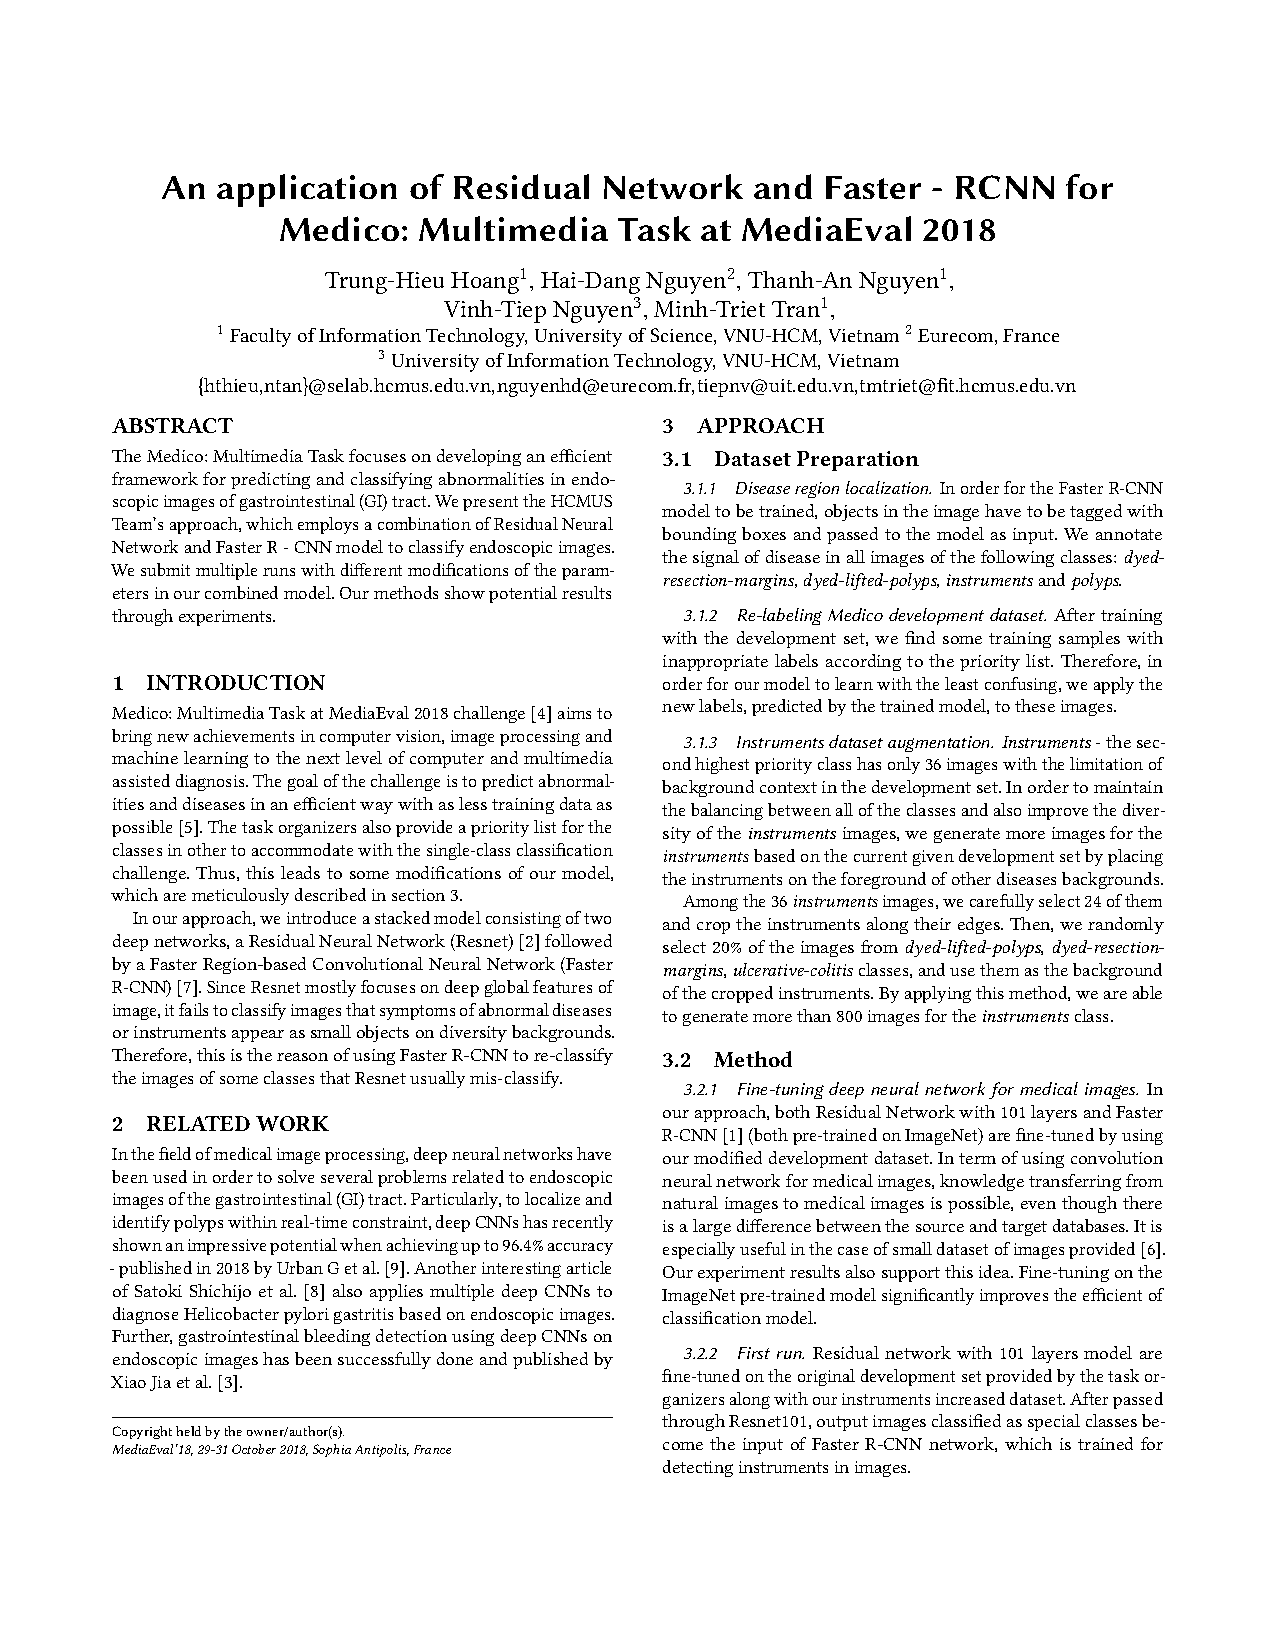
\includepdf[page=-]{publications/hthieu_media_eval_2018.pdf}
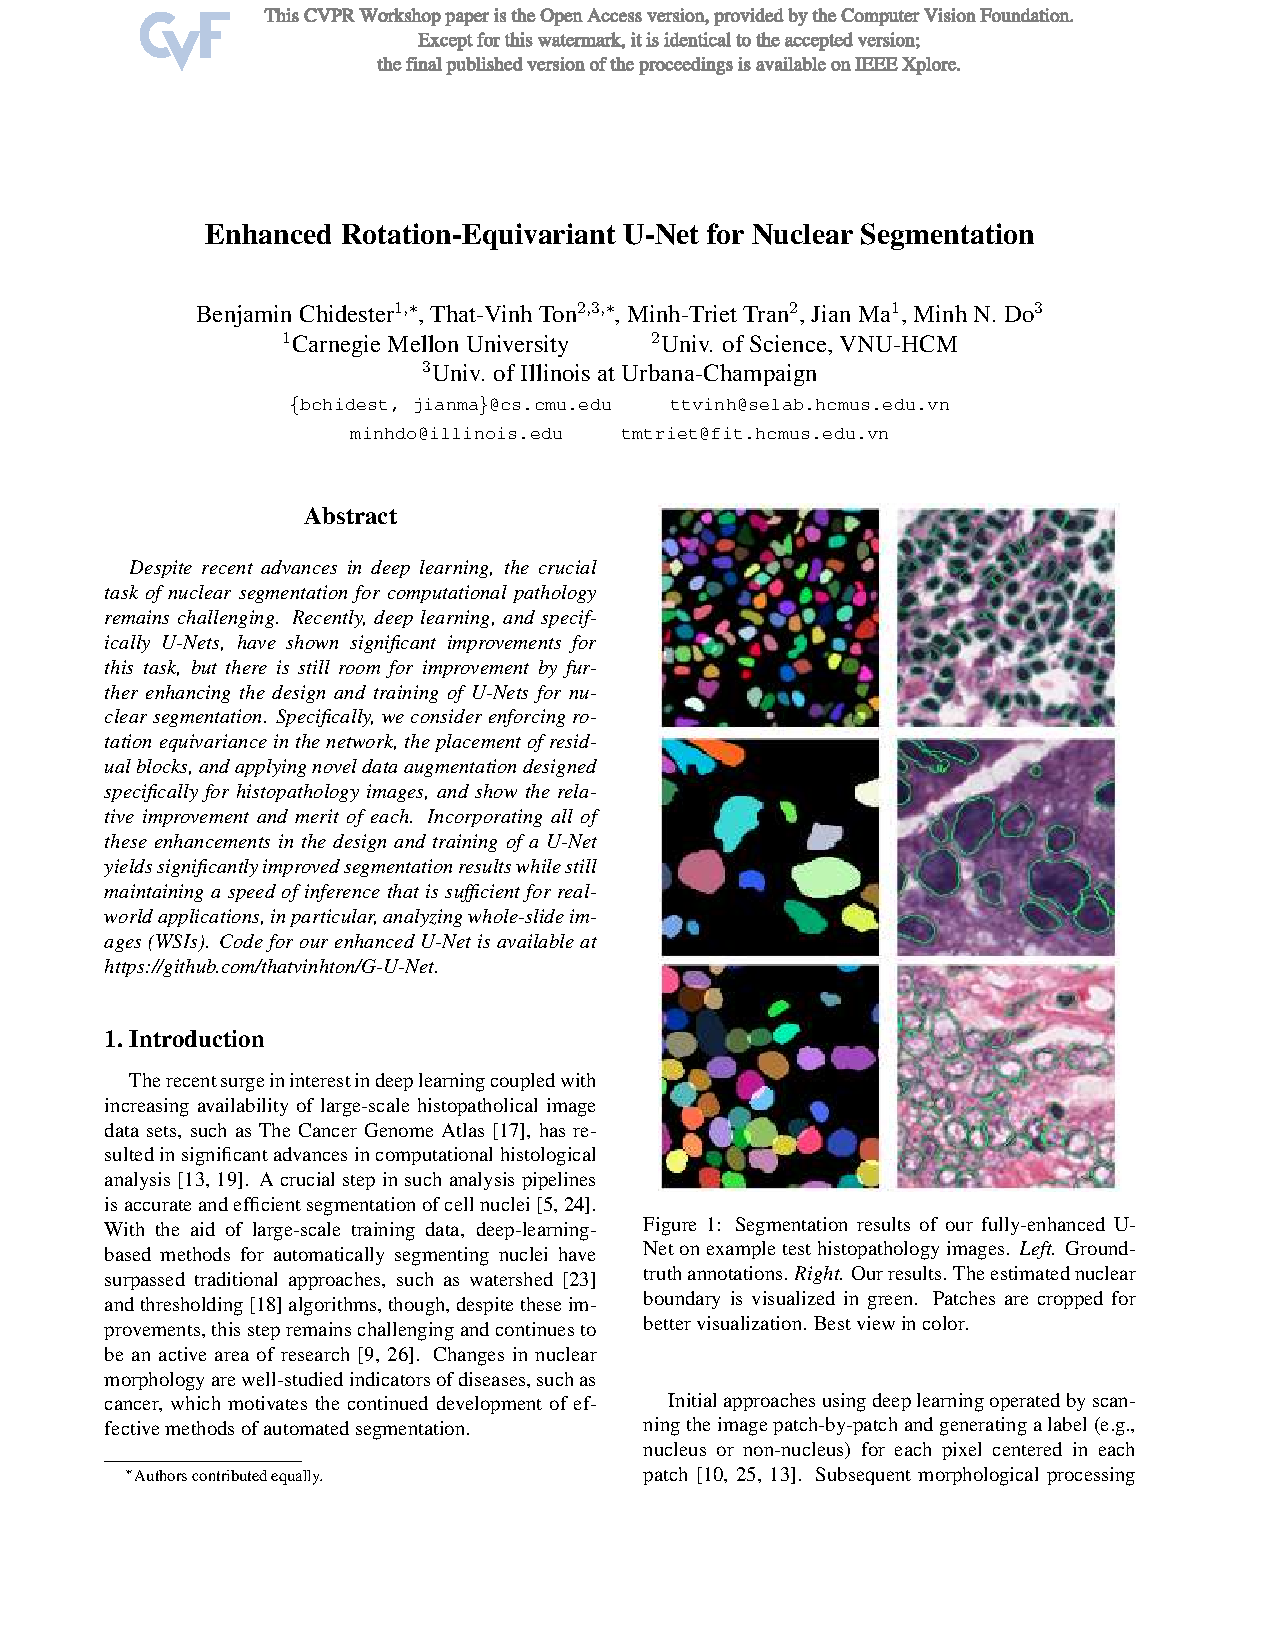
\includepdf[page=-]{publications/Chidester_Enhanced_Rotation-Equivariant_U-Net_for_Nuclear_Segmentation_CVPRW_2019_paper.pdf}
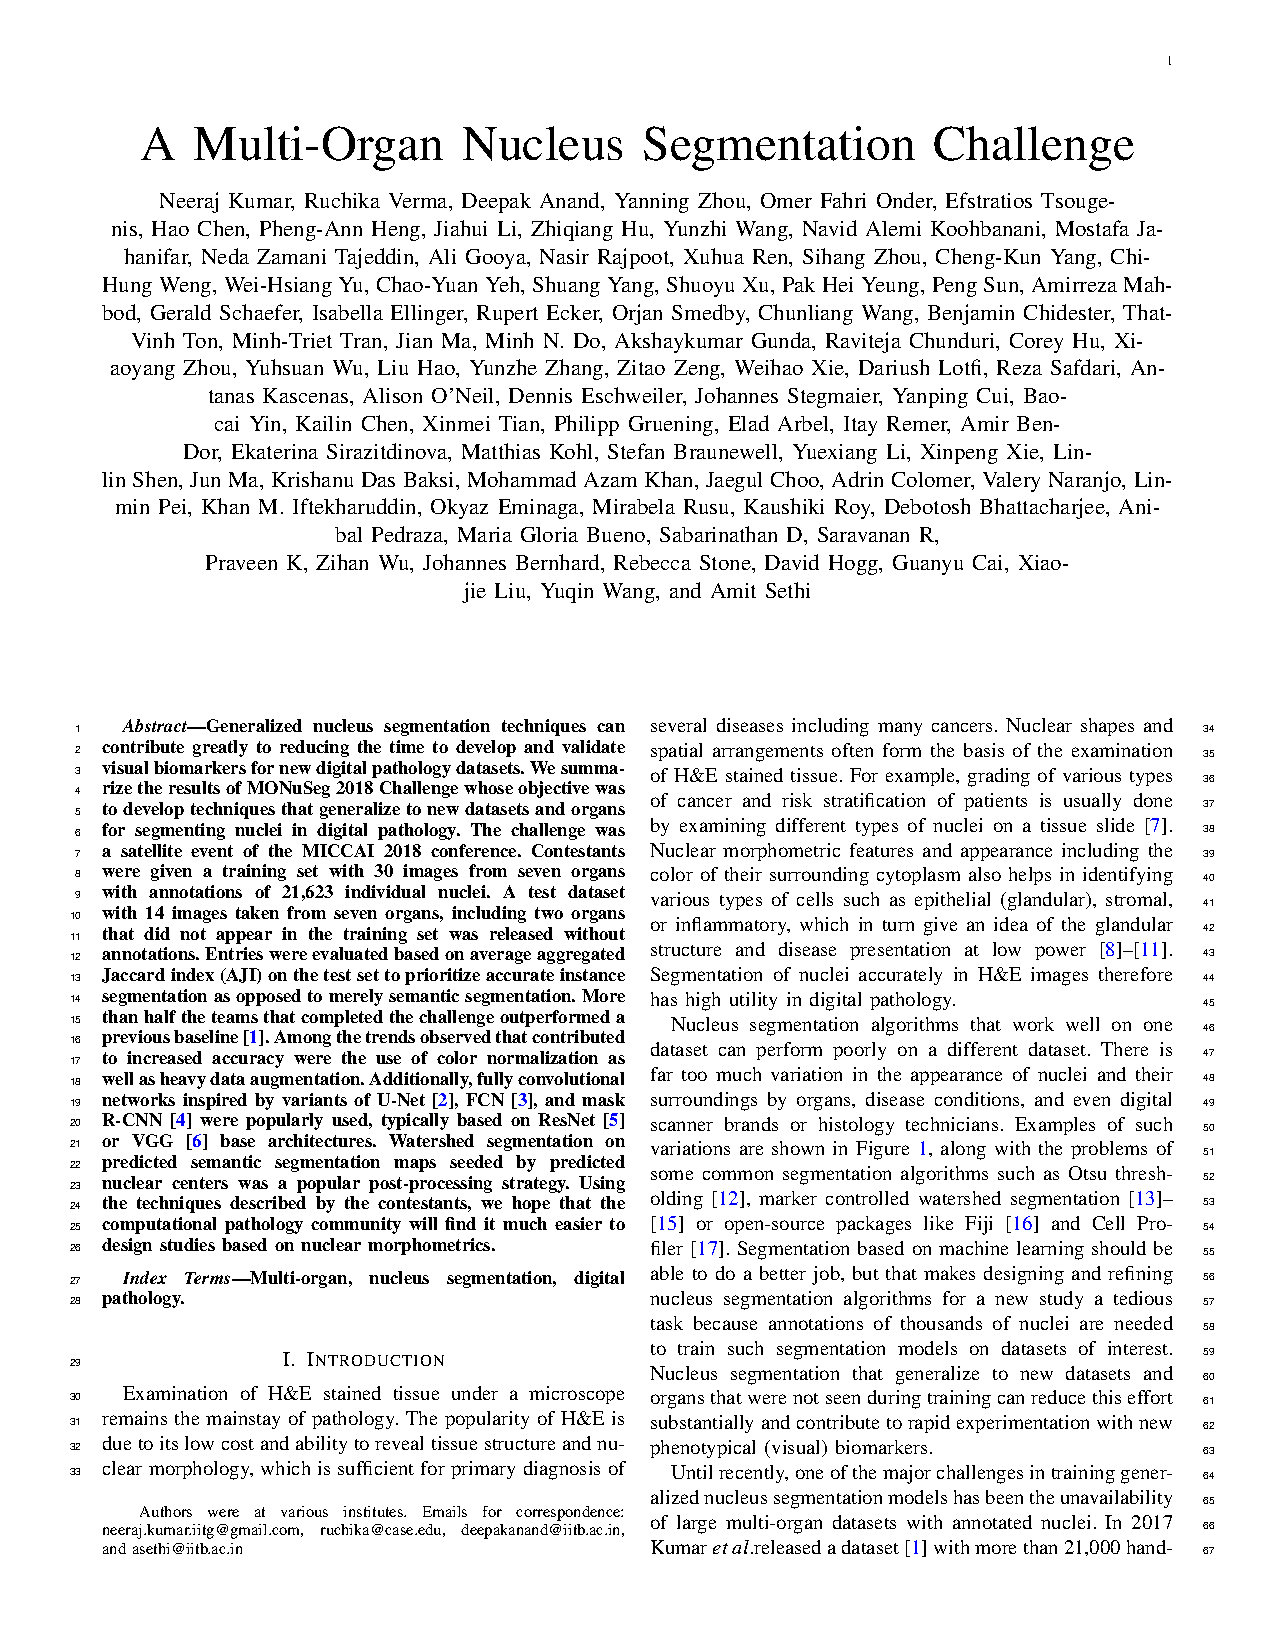
\includepdf[page=-]{publications/Manucript_MoNuseg_v1_0_14March2019.pdf}
\includepdf[page=-]{publications/hthieu_BioMedia_2019.pdf}



\end{document}
